% Ce fichier main.tex est le fichier principal \`{a} partir duquel tout est g\'{e}n\'{e}r\'{e}
% This file is the main file where the final document is generated
\documentclass{these-dbl}

% Remplir les metadonnees du pdf
% Fill the pdf metadata
\hypersetup{
   pdfauthor   = {William PENSEC},
   pdftitle    = {Protection d'un processeur avec DIFT contre des attaques physiques},
   pdfsubject  = {Th\`{e}se de doctorat de William PENSEC},
   pdfkeywords = {},
   pdfstartview= {FitV} % ajuste la page à la largueur de l'écran
}

\geometry{vmargin=4.0cm}
\definecolor{backcolour}{rgb}{0.98,0.98,0.98}
\definecolor[named]{LightGray}{RGB}{230,230,230}

\lstset{
  aboveskip=0.25cm,
  belowskip=0mm,
  basicstyle=\tiny,
  backgroundcolor=\color{backcolour},
  breakatwhitespace=false,
  breaklines=true,
  captionpos=t,
  commentstyle=\color{gray},
  deletekeywords={...},
  escapeinside={\%*}{*)},
  extendedchars=true,
  framexleftmargin=1pt,
  framextopmargin=0pt,
  framexbottommargin=0pt,
  frame=tb,
  keepspaces=true,
  keywordstyle=\color{red},
  language=C,
  literate=
  {²}{{\textsuperscript{2}}}1
  {⁴}{{\textsuperscript{4}}}1
  {⁶}{{\textsuperscript{6}}}1
  {⁸}{{\textsuperscript{8}}}1
  {€}{{\euro{}}}1
  {é}{{\'e}}1
  {è}{{\`{e}}}1
  {ê}{{\^{e}}}1
  {ë}{{\"{e}}}1
  {É}{{\'{E}}}1
  {Ê}{{\^{E}}}1
  {û}{{\^{u}}}1
  {ù}{{\`{u}}}1
  {â}{{\^{a}}}1
  {à}{{\`{a}}}1
  {á}{{\'{a}}}1
  {ã}{{\~{a}}}1
  {Á}{{\'{A}}}1
  {Â}{{\^{A}}}1
  {Ã}{{\~{A}}}1
  {ç}{{\c{c}}}1
  {Ç}{{\c{C}}}1
  {õ}{{\~{o}}}1
  {ó}{{\'{o}}}1
  {ô}{{\^{o}}}1
  {Õ}{{\~{O}}}1
  {Ó}{{\'{O}}}1
  {Ô}{{\^{O}}}1
  {î}{{\^{i}}}1
  {Î}{{\^{I}}}1
  {í}{{\'{i}}}1
  {Í}{{\~{Í}}}1,
  morekeywords={},
  numbers=left,
  numbersep=10pt,
  numberstyle=\tiny\color{black},
  rulecolor=\color{black},
  showspaces=false,
  showstringspaces=false,
  showtabs=false,
  stepnumber=1,
  stringstyle=\color{gray},
  tabsize=4,
  title=\lstname
}

\lstdefinestyle{topPosition}{
  float=ht,
  floatplacement=ht
}

\lstdefinelanguage[RISC-V]{Assembler}
{
  alsoletter={.}, % allow dots in keywords
  alsodigit={0x}, % hex numbers are numbers too!
  morekeywords=[1]{ % instructions
    lb, lh, lw, lbu, lhu,
    sb, sh, sw,
    sll, slli, srl, srli, sra, srai,
    add, addi, sub, lui, auipc,
    xor, xori, or, ori, and, andi,
    slt, slti, sltu, sltiu,
    beq, bne, blt, bge, bltu, bgeu,
    j, jr, jal, jalr, ret,
    scall, break, nop, 
    csrr
  },
  morekeywords=[2]{ % sections of our code and other directives
    .align, .ascii, .asciiz, .byte, .data, .double, .extern,
    .float, .globl, .half, .kdata, .ktext, .set, .space, .text, .word, mcycle
  },
  morekeywords=[3]{ % registers
    zero, ra, sp, gp, tp, s0, fp,
    t0, t1, t2, t3, t4, t5, t6,
    s1, s2, s3, s4, s5, s6, s7, s8, s9, s10, s11,
    a0, a1, a2, a3, a4, a5, a6, a7,
    ft0, ft1, ft2, ft3, ft4, ft5, ft6, ft7,
    fs0, fs1, fs2, fs3, fs4, fs5, fs6, fs7, fs8, fs9, fs10, fs11,
    fa0, fa1, fa2, fa3, fa4, fa5, fa6, fa7,
    x0, x1, x2, x3, x4, x5, x6, x7, x8, x9, 
    x10, x11, x12, x13, x14, x15, x16, x17, x18, x19,
    x20, x21, x22, x23, x24, x25, x26, x27, x28, x29,
    x30, x31
  },
  morecomment=[l]{;},   % mark ; as line comment start
  morecomment=[l]{\#},  % as well as # (even though it is unconventional)
  morestring=[b]",      % mark " as string start/end
  morestring=[b]'       % also mark ' as string start/end
}

% usage example:

% define some basic colors
\definecolor{mauve}{rgb}{0.58,0,0.82}

% \lstset{
%   basicstyle=\tiny\ttfamily,                    % very small code
%   breaklines=true,                              % break long lines
%   commentstyle=\itshape\color{green!50!black},  % comments are green
%   keywordstyle=[1]\color{blue!80!black},        % instructions are blue
%   keywordstyle=[2]\color{orange!80!black},      % sections/other directives are orange
%   keywordstyle=[3]\color{red!50!black},         % registers are red
%   stringstyle=\color{mauve},                    % strings are from the telekom
%   identifierstyle=\color{teal},                 % user declared addresses are teal
%   frame=l,                                      % black line on the left side of code
%   language=[RISC-V]Assembler,                   % all code is RISC-V
%   tabsize=4,                                    % indent tabs with 4 spaces
%   showstringspaces=false                        % do not replace spaces with weird underlines
% }
\newboolean{showcomments}
% \setboolean{showcomments}{false}
\setboolean{showcomments}{true}
\ifthenelse{\boolean{showcomments}}
{ \newcommand{\mynote}[2]{
    \fbox{\bfseries\sffamily\normalsize#1}
    {\normalsize$\blacktriangleright$\textsf{\emph{#2}}$\blacktriangleleft$}}}
{ \newcommand{\mynote}[2]{}}

\newcommand{\wip}[1]{\mynote{William}{\textcolor{red}{#1}}}
\newcommand{\vl}[1]{\mynote{Vianney}{\textcolor{blue}{#1}}}
\newcommand{\gug}[1]{\mynote{Guy}{\textcolor{ForestGreen}{#1}}}

%%%%%%%%%%%%%%%%%%%%%%%%%%%%%%%%%%%%%%%%%%%%%%%%%%%%%%%%%%%%%%%%%%%%%%%%%%%%%%%%%%%%%%%%%%%%%%%%%%%%%%%%%%%%%%%%%%%%%%%%%%%%%%%
\makenomenclature
\renewcommand{\nomname}{Acronyms}
\nomenclature{FIA}{Fault Injection Attack}
\nomenclature{SCA}{Side Channel Attack}
\nomenclature{TPR}{Tag Propagation Register}
\nomenclature{TCR}{Tag Check Register}
\nomenclature{CSR}{Control and Status Registers}
\nomenclature{DIFT}{Dynamic Information Flow Tracking}
\nomenclature{RA}{Return Address}
\nomenclature{PC}{Program Counter}
\nomenclature{ISA}{Instruction Set Architecture}
\nomenclature{CABA}{Cycle Accurate and Bit Accurate}
\nomenclature{OS}{Operating System}
\nomenclature{GUI}{Graphical User Interface}
\nomenclature{API}{Application Programming Interface}
\nomenclature{FPGA}{Field Programmable Gate Array}
\renewcommand\_{\textunderscore\allowbreak}

% Spécifier vos fichiers de bibliographie
% Specify you bibliography files here
\addbibresource{./biblio/biblio.bib}

\setlength{\headheight}{14pt}

%%%%%%%%%%%%%%%%%%%%% Minitoc configuration %%%%%%%%%%%%%%%%%%%%%
\setcounter{minitocdepth}{2}
\usepackage{lipsum}

%%%%%%%%%%%%%%%%%%%%% Epigraph configuration %%%%%%%%%%%%%%%%%%%%%
\usepackage{calrsfs}
\usepackage{dutchcal}
% Set the desired width for the epigraph
\setlength{\epigraphwidth}{0.8\textwidth}

\begin{document}
\addtocontents{toc}{\protect\hypertarget{toc}{}}

% Page de garde avec commande \maketitle
% Front cover calling \maketitle
% La page de garde est en français
% The front cover is in French
\selectlanguage{french}

% Inclure les infos de chaque établissement
% Include each institution data

%%% Switch case in latex
%%% https://tex.stackexchange.com/a/343306
\makeatletter
\newcommand\addcase[3]{\expandafter\def\csname\string#1@case@#2\endcsname{#3}}
\newcommand\makeswitch[2][]{%
  \newcommand#2[1]{%
    \ifcsname\string#2@case@##1\endcsname\csname\string#2@case@##1\endcsname\else#1\fi%
  }%
}
\makeatother

%%%% Il faut adapter la taille des logos dans certains cas (e.g., EGAAL, 2 etablissements)
\newcommand\hauteurlogos[3]{
    \hauteurlogoecole{#1}
    \hauteurlogoetablissementA{#2}
    \hauteurlogoetablissementB{#3}
}

%%%%%%%%%%%%%%%%%%%%%%%%%%%%%%%%%%%%%%%%%%%%%%%%%%%
%%%%%%%%%%%%%%%% ECOLES DOCTORALES %%%%%%%%%%%%%%%%

%%%% #1: dossier des images, #2: numero ED, #3: couleur ED, #4-#5: nom complet sur plusieurs lignes
\newcommand\addecoledoctorale[5]{\direcole{#1}\numeroecole{#2}\definecolor{color-ecole}{RGB}{#3}\nomecoleA{#4}\nomecoleB{#5}}

\makeswitch[default]\ecoledoctorale{}

\addcase\ecoledoctorale{MathSTIC}{\addecoledoctorale
    {MathSTIC}
    {644}
    {159,182,217} %{236,115,127}
    {Math\'{e}matiques et Sciences et Technologies}
    {de l'Information et de la Communication en Bretagne Océane}
}

%%%%%%%%%%%%%%%%%%%%%%%%%%%%%%%%%%%%%%%%%%%%%%%%
%%%%%%%%%%%%%%%% ETABLISSEMENTS %%%%%%%%%%%%%%%%

%%%% #1 nom du logo, #2-#4: nom complet sur plusieurs lignes
\newcommand\addetablissement[4]{\logoetablissementB{#1}\nometablissementC{#2}\nometablissementD{#3}\nometablissementE{#4}}

\makeswitch[default]\etablissement{}

\addcase\etablissement{ENIB}{\addetablissement
    {ENIB}
    {}
    {L'\'{E}COLE NATIONALE}
    {D'ING\'{E}NIEURS DE BREST}
}

\addcase\etablissement{UBO}{\addetablissement
    {UBO}
    {}
    {}
    {L'UNIVERSIT\'{E} DE BRETAGNE OCCIDENTALE}
}
\addcase\etablissement{UBS}{\addetablissement
    {UBS}
    {}
    {}
    {L'UNIVERSIT\'{E} DE BRETAGNE SUD}
}



% Inclure infos de l'école doctorale
% Include doctoral school data
\ecoledoctorale{MathSTIC}

% Inclure infos de l'établissement
% Include institution data
\etablissement{UBS}

%Inscrivez ici votre sp\'{e}cialit\'{e} (voir liste des sp\'{e}cialit\'{e}s sur le site de votre \'{e}cole doctorale)
%Indicate the domain (see list of domains in your ecole doctorale)
\spec{Informatique et Architectures Numériques}

%Attention : le pr\'{e}nom doit être en minuscules (Jean) et le NOM en majuscules (BRITTEF) 
%Attention : the first name in small letters and the name in Capital letters 
\author{William PENSEC}

% Donner le titre complet de la th\`{e}se, \'{e}ventuellement le sous titre, si n\'{e}cessaire sur plusieurs lignes 
%Give the complete title of the thesis, if necessary on several lines
\title{Extension de la Protection des Processeurs Contre les Menaces Physiques et Logicielles par la Sécurisation du Mécanisme DIFT Contre les Attaques par Injections de Fautes}
\lesoustitre{Enhanced Processor Defence Against Physical and Software Threats by Securing DIFT Against Fault Injection Attacks}

%Indiquer la date et le lieu de soutenance de la th\`{e}se 
%indicates the date and the place of the defense 
\date{19/12/2024}
\lieu{Lorient}

%Indiquer le nom du (ou des) laboratoire (s) dans le(s)quel(s) le travail de th\`{e}se a \'{e}t\'{e} effectu\'{e}, indiquer aussi si souhait\'{e} le nom de la (les) facult\'{e}(s) (UFR, \'{e}cole(s), Institut(s), Centre(s)...), son (leurs) adresse(s)... 
%Indicates the name (or names) of research laboratories where the work has been done as well as (if desired) the names of faculties (UFR, Schools, institution...
\uniterecherche{UMR CNRS 6285, Lab-STICC, Université Bretagne Sud}

%Indiquer le Numero de th\`{e}se, si cela est opportun, ou laisser vide pour faire disparaitre cet ligne de la couverture
%Indicate the number of the thesis if there is one. otherwise leave empty so the line disappeurs on the cover
\numthese{« si pertinent »} % \numthese{}

%Indiquer le Pr\'{e}nom en minuscules et le Nom en majuscules, le titre de la personne et l’\'{e}tablissement dans lequel il effectue sa recherche  
%Indicates the first name on small letters and the Names on capital letters, the person's title and the institution where he/she belongs to.
%Exemples :  Examples :
%%%- Professeur, Universit\'{e} d’Angers 
%%%- Chercheur, CNRS, \'{e}cole Centrale de Nantes 
%%%-  Professeur d’universit\'{e} – Praticien Hospitalier, Universit\'{e} Paris V  
%%%-  Maitre de conf\'{e}rences, Oniris 
%%%- Charg\'{e} de recherche, INSERM, HDR, Universit\'{e} de Tours  
 %S’il n’y a pas de co-direction, faire disparaitre cet item de la couverture  
 %In there is no co-director, remove the item from the cover
\jury{
% {\normalTwelve \textbf{Rapporteurs avant soutenance :}}\\ \newline
% \footnotesizeTwelve
% \begin{tabular}{@{}ll}
% Pr\'{e}nom NOM & Fonction et \'{e}tablissement d'exercice \\
% Pr\'{e}nom NOM & Fonction et \'{e}tablissement d'exercice \\
% Pr\'{e}nom NOM & Fonction et \'{e}tablissement d'exercice \\
% \end{tabular}

{\normalTwelve \textbf{Rapporteurs avant soutenance :}}\\ \newline
\footnotesizeTwelve
\begin{tabular}{@{}ll}
Lejla BATINA & Professeur des Universités (Radboud University, Pays-Bas) \\
Nele MENTENS & Professeur des Universités (Leiden University et KU Leuven, Belgique) \\
Vincent BEROULLE & Professeur des Universités (LCIS, Université Grenoble Alpes, France) \\
\end{tabular}

\vspace{\baselineskip}
{\normalTwelve \textbf{Composition du Jury :}}\\ \newline
% {\fontsize{9.5}{11}\selectfont {\textcolor{red}{\textit{Attention, en cas d’absence d’un des membres du Jury le jour de la soutenance, la composition du jury doit être revue pour s’assurer qu’elle est conforme et devra être répercutée sur la couverture de thèse}}}}\\ \newline
\footnotesizeTwelve
\begin{tabular}{@{}lll}

Pr\'{e}sident :        & Pr\'{e}nom NOM & Fonction et \'{e}tablissement d'exercice \textit{(à préciser après la soutenance)} \\
Examinateurs :         & Pr\'{e}nom NOM & Fonction et \'{e}tablissement d'exercice \\
Dir. de th\`{e}se :    & Guy GOGNIAT & Professeur des Universités (Lab-STICC, Université Bretagne Sud, Lorient, France) \\
Co-dir. de th\`{e}se : & Vianney LAP\^OTRE & Maitre de Conférence HDR (Lab-STICC, Université Bretagne Sud, Lorient, France) \\
\end{tabular}

% \vspace{\baselineskip}
% {\normalTwelve \textbf{Composition du Jury :}}\\
% {\fontsize{9.5}{11}\selectfont {\textcolor{red}{\textit{Attention, en cas d’absence d’un des membres du Jury le jour de la soutenance, la composition du jury doit être revue pour s’assurer qu’elle est conforme et devra être répercutée sur la couverture de thèse}}}}\\ \newline
% \footnotesizeTwelve
% \begin{tabular}{@{}lll}

% Pr\'{e}sident :        & Pr\'{e}nom NOM & Fonction et \'{e}tablissement d'exercice \textit{(à préciser après la soutenance)} \\
% Examinateurs :         & Jean-Max DUTERTRE & Professeur des Universités (Ecole des Mines de Saint-Etienne) \\
%                        & Francesco REGAZZONI & Professeur des Universités (University of Amsterdam et\\ && Università della Svizzera italiana) \\
% Dir. de th\`{e}se :    & Guy GOGNIAT & Professeur des Universités (Lab-STICC, Université Bretagne Sud) \\
% Co-dir. de th\`{e}se : & Vianney LAP\^OTRE & Maitre de Conférence HDR (Lab-STICC, Université Bretagne Sud) \\
% \end{tabular}

% \vspace{\baselineskip}
% {\normalTwelve \textbf{Invit\'{e}(s) :}}\\ \newline
% \footnotesizeTwelve
% \begin{tabular}{@{}ll}
% Pr\'{e}nom NOM & Fonction et \'{e}tablissement d'exercice \\
% \end{tabular}
}

\maketitle


% Sélectionner la langue du contenu suivant cette ligne
% Select the content language following this line
\selectlanguage{english}

% \setlength{\headheight}{14pt}
% \addtolength{\topmargin}{-1.6pt}

\thispagestyle{empty}
\pagenumbering{roman}

% Inclusion du chapitre remerciement
% Input acknowledgement chapter
\clearemptydoublepage
\vspace*{\fill}

\epigraph{{\large $\mathcal{A}$d mentes inquisitivas quae lucem futuri Scientiae accendunt.}\\
{\footnotesize \textit{Aux esprits curieux qui illuminent l'avenir de la Connaissance.}}\\
{\footnotesize \textit{To the inquisitive minds that are lighting up the future of Knowledge.}}}{}

\vspace*{\fill}

% Inclusion du chapitre remerciement
% Input acknowledgement chapter
% \clearemptydoublepage
\chapter*{Remerciements}

Tout d'abord, je tiens à remercier mon directeur de thèse, Guy Gogniat, Professeur des Universités, ainsi que mon codirecteur de thèse, Vianney Lapôtre, Maitre de Conférences HDR, tous les deux à l'Université Bretagne Sud, à Lorient. Leur accompagnement, expertise et soutien ont été plus que précieux durant cette thèse.

Je remercie également Lejla Batina, Nele Mentens et Vincent Beroulle, respectivement Professeurs des Universités à Radboub (Pays-Bas), KU leuven (Belgique), et à Grenoble, pour avoir accepté de rapporter ma thèse. Leurs remarques ont été pertinentes et m'ont permis d'améliorer mon manuscrit.

Je souhaite également remercier Jean-Max Dutertre, Professeur à l'\'Ecole des Mines de Saint-\'Etienne, à Gardanne, qui a accepté de participer à mon Comité de Suivi de thèse (CSI) ainsi que d'avoir accepté de faire partie de mon jury de thèse. Je remercie également Karine Heydemann pour avoir fait partie de mon CSI.

Je remercie grandement Francesco Regazzoni, Professeur à l'Università della Svizzera Italiana, à Lugano (Suisse) et à l'Université d'Amsterdam (Pays-Bas) pour avoir accepté de faire partie de mon jury de thèse et pour m'avoir guidé durant ma mobilité. J'ai beaucoup apprécié les échanges que nous avons pu avoir. Cela a contribué positivement à mon travail, la preuve étant avec les contributions scientifiques que cela a amené. Cela m'a permis d'étendre mes connaissances en sécurité ainsi que d'améliorer mon anglais. J'ai pu rencontrer de nouveaux chercheurs, doctorants et postdoctorants au laboratoire et d'échanger avec eux, ce qui m'a enrichi personnellement et professionnellement. J'ai eu la chance de découvrir un endroit formidable durant ces cinq mois et d'en garder un souvenir incroyable. J'espère pouvoir y retourner bientôt.

De plus, je souhaite remercier mes collègues au Lab-STICC, Nicolas, Mohamed, Noura, Hongwei, Tianxu, Clément, et tous les autres, ainsi que les personnes que j'ai pu rencontrer durant ma thèse. Un grand merci à Tom et Chiara, rencontrés lors de mon séjour à Lugano. Ils m'ont tous deux aidé à m'intégrer dans cette nouvelle ville. Nous avons également eu des discussions très intéressantes. Je vous dis à bientôt, j'espère. Je souhaite enfin remercier mes enseignants de Licence et Master (particulièrement Catherine Dezan et David Espès) à l'Université de Bretagne Occidentale d'avoir cru en moi et m'avoir offert la possibilité de réaliser des stages en recherche.

Finalement, je conclurai en remerciant mes parents, mon frère, ma copine Hellen, ma famille, ainsi que tous mes amis pour leur support et leur accompagnement pendant toutes ces années. Merci pour vos remarques, vos conseils et votre écoute. Vous m'avez tous permis de mener à bien ce travail jusqu'au bout en me permettant de me sentir toujours bien.
Merci pour tout.

\chapter*{Acknowledgments}

Firstly, I would like to thank my thesis supervisor, Professor Guy Gogniat, and my co-supervisor, Vianney Lapôtre, Associate Professor, both at the Université Bretagne Sud in Lorient (France). Their guidance, expertise, and support have been invaluable during this thesis.

Secondly, I would like to thank Lejla Batina, Nele Mentens and Vincent Beroulle, respectively Full Professors at Radboub University (Netherlands), KU Leuven (Belgium) and Grenoble (France), for agreeing to review my PhD thesis. Their comments were pertinent and helped me to improve my manuscript.

I would also like to thank Jean-Max Dutertre, Professor at the Ecole des Mines de Saint-Étienne, Gardanne, who agreed to take part in my thesis monitoring committee (Comité de Suivi de thèse - CSI) and to sit on my thesis jury. I would also like to thank Karine Heydemann for being part of my CSI.

I would like to thank Francesco Regazzoni, Senior Researcher at the Università della Svizzera Italiana in Lugano (Switzerland) and at the University of Amsterdam (Netherlands), for agreeing to sit on my thesis jury and for guiding me during my mobility. I very much appreciated the exchanges we had. It made a positive contribution to my work, as evidenced by the scientific contributions it brought. It enabled me to broaden my knowledge of security and improve my English. I was able to meet new researchers, PhD students and post-docs in the laboratory and exchange ideas with them, which enriched me personally and professionally. I've been lucky enough to discover a wonderful place, in Lugano, during these five months and to have incredible memories of it. I hope to be able to return there very soon.

I would also like to thank my colleagues at the Lab-STICC, Nicolas, Mohamed, Noura, Hongwei, Tianxu, Clément, and all the others, as well as the people I met during my thesis. A big thanks to Tom and Chiara, whom I met during my stay in Lugano. They both helped me at the time to integrate myself in this new city. We also had some very interesting and rewarding discussions. I hope to see you soon. Finally, I'd like to thank my undergraduate and Master's teachers (especially Prof. Boukhobza, Dr. Dezan, Prof. Espès) at the Université de Bretagne Occidentale for believing in me and giving me the opportunity to do research internships.

Finally, I would like to conclude by thanking my parents, my brother, my girlfriend Hellen, my family and all my friends for their support and guidance over the years. Thank you for your comments, advice, and attentiveness. You have all enabled me to see this work through to the end, making me always feel good.

Thank you very much for everything.

% Ne pas oublier cette commande qui g\'{e}n\`{e}re la page de couverture avant
% This command will generate the front cover
\frontmatter
\clearemptydoublepage
\renewcommand{\contentsname}{Table of Contents}
\addcontentsline{toc}{chapter}{Table of Contents}
\dominitoc % Initialization
\tableofcontents %sommaire %table of content
%\shorttableofcontents{Sommaire}{0}

\printnomenclature
\listoffigures
\addcontentsline{toc}{chapter}{List of Figures}
\listoftables
\addcontentsline{toc}{chapter}{List of Tables}
\renewcommand{\lstlistlistingname}{List of Listings}
\lstlistoflistings
\addcontentsline{toc}{chapter}{List of Listings}

%%%%%%%%%%%%%%%%%%%%%%%%%%%%%%%%%%%%%%%%%%%%%%%%%%%%%%%%%%%%%%%%%%%%%%%%%%%%%%%%%%%%%%%%%%%%%%%%%%%%%%%%%%%%%%%%%%%%%%%%%%%%%%%%%%%%%%%%%%%%

\clearemptydoublepage
\pagenumbering{arabic}
\setcounter{page}{1}
\setcounter{mtc}{5}
\mainmatter
\input{./c1_intro/Introduction}

\clearemptydoublepage
\chapter{State of the Art}
\chaptermark{State of the Art}
\label{chapter:soa}
\minitoc

%%%%%%%%%%%%%%%%%%%%%%%%%%%%%%%%%%%%%%%%%%%%%%%%%%%%%%%%%%%%%%%%%%%%%%%%%%%%%%%%%%%%%%%%%%%%%%%
\section{Introduction}
This chapter provides an overview of related work to contextualize the primary objectives of this thesis. Firstly, in Section~\ref{section:ift}, Information Flow Tracking (IFT) is introduced, detailing the different types and their respective purposes. We discuss the various levels of monitoring, from program behaviour to the detection of hardware trojans.
Then in Section~\ref{section:physicalAttacks}, Physical Attacks are examined, focusing on two main types: Side-Channel Attacks (SCA) and Fault Injection Attacks (FIA).
Finally in Section~\ref{section:countermeasuresAgainstFIA}, as this work concentrate on FIA, we exclusively present countermeasures against Fault Injection Attacks.

%%%%%%%%%%%%%%%%%%%%%%%%%%%%%%%%%%%%%%%%%%%%%%%%%%%%%%%%%%%%%%%%%%%%%%%%%%%%%%%%%%%%%%%%%%%%%%%
\section{Information Flow Tracking}
\label{section:ift}
The concept of \textit{Information Flow Tracking} has been introduced by the work of Bell and LaPadula~\cite{BLP-76-military} and by Denning~\cite{D-76-commacm} in 1976.
This section introduces Information Flow Tracking mechanisms, explains how they work, and presents the various types of IFT with their different functional levels.
    
%%%%%%%%%%%%%%%%%%%%%%%%%%%%%%%%
\subsection{Different types of IFT}
There are two distinct types of IFT approaches: static and dynamic, each with its own specific objectives.

\subsubsection{Static IFT}
Static Information Flow Tracking (SIFT) is a security technique used to analyse and control the flow of information within a program or system without executing it, by examining the source code or compiled binary~\cite{HAK-21-acmcsur}. This method is particularly useful for identifying theoretical vulnerabilities, ensuring compliance with design principles, and preventing unauthorised information leaks before deployment. SIFT is comprehensive, covering all possible execution paths and detecting both explicit information flows (direct data assignments) and implicit flows (leaks through control flow structures). By performing checks at compile-time, SIFT helps developers address potential security issues early, enforcing principles like non-interference and data confidentiality through security policies. However, static analysis may generate false positives by flagging theoretical flows that might not occur in practice and may struggle with certain dynamic language features or runtime-dependent behaviours. SIFT is employed in various contexts, such as verifying secure information flow in operating systems, programming languages with built-in information flow controls, and hardware design for secure systems.

\subsubsection{Dynamic IFT}
Dynamic Information Flow Tracking (DIFT) is a powerful security technique that monitors and analyses, in real-time, the flow of information within a program during its execution~\cite{CGDJ-21-micromac}. DIFT operates by tagging or labelling input data from potentially untrusted sources and tracking how this data propagates through the system~\cite{SLD-04-sigplan}. As the program executes, DIFT maintains metadata about the tagged information, updating it as operations are performed on the data. This allows the system to detect when tainted data is used in security-critical operations, such as modifying control flow or accessing sensitive resources. DIFT can be implemented at various levels, including hardware, software, or a combination of both. Hardware-based implementations often offer better performance but require specialized processor modifications, while software-based approaches provide more flexibility but may incur higher overhead~\cite{CGDJ-21-micromac}. DIFT has proven effective in detecting and preventing a wide range of security vulnerabilities, including buffer overflows, format string attacks, and code injection attacks~\cite{SLD-04-sigplan}. However, DIFT also faces challenges, such as handling implicit information flows, managing performance overhead, and addressing over-tainting issues.
This approach might not cover all potential data paths, as it is dependent on the specific conditions and inputs provided during the monitoring period.
Despite these challenges, DIFT remains a valuable tool for software security, particularly for runtime attack detection in modern systems.

%%%%%%%%%%%%%%%%%%%%%%%%%%%%%%%%    
\subsection{Different levels of DIFT}
IFT can be implemented at various levels of abstraction in computing systems~\cite{HAK-21-acmcsur, BSMCVEJCO-21-acmcsur,CGDJ-21-micromac}. Each level presents unique trade-offs between precision, performance overhead, and ease of implementation, allowing designers to choose the most appropriate approach for their security requirements.

Software-based DIFT mechanisms benefit from close integration with the software context via binary code instrumentation and source code modifications, offering better flexibility, customisation, and scalability without altering hardware components. However, these software solutions often incur high performance overheads due to the extra instructions required. They operate at either the system level, monitoring OS-wide information flows, or the program level, focusing on specific applications.
On the other hand, hardware-assisted DIFT designs can efficiently enforce security rules by implementing DIFT-related operations as hardware logic, reducing performance overhead but at the expense of flexibility and scalability, making them challenging to deploy in modern commercial systems. They can be implemented within processor cores or as off-core designs. But they can also be at the lowest level, such as Gate-Level IFT who tracks information flow through logic gates.
A hybrid hardware and software co-design offers a promising alternative, enabling fine-grained security checks by associating software context with hardware data, though it faces challenges such as balancing flexibility with hardware overhead and designing appropriate tags that support rule updates post-deployment.

Figure~\ref{fig:levels_system} represents the different levels of a simplified embedded system: application layer, system service layer, OS layer, and hardware layer. This figure is inspired by Figure 1.9 of~\cite{ebrary}. Software-based IFTs work in the first three levels.

Positioned at the highest level of the software hierarchy, \textit{the application layer} is responsible for implementing system functionalities and business logic. Functionally, all modules within this layer work together to execute the required system operations. Applications generally run in a less-privileged mode on the processor and utilise the OS-provided API scheduling to communicate with the operating system.
\textit{The system service layer} serves as the intermediary service interface offered by the OS to the application layer. This interface allows applications to access a variety of OS-provided services, essentially bridging the gap between the OS and applications. Typically, this layer encompasses components like the file system, Graphical User Interface (GUI), task manager.
An Operating System (OS) is a software framework designed to manage hardware resources uniformly. It abstracts numerous hardware functions and offers them to applications as services. Common services provided by an OS include scheduling, file synchronisation, and networking. Operating systems are prevalent in both desktop and embedded systems. In the context of embedded systems, OSs possess distinct characteristics such as stability, customisability, modularity, and real-time processing capabilities.
\textit{The hardware layer} refers to the physical components and circuitry, including the microprocessor or microcontroller, memory, sensors, and input/output interfaces. This layer encompasses all the tangible electronic elements that interact directly with each other to perform the device's functions. It provides the essential infrastructure that supports and drives the embedded system’s operations and connectivity.

\begin{figure}[ht]
    \centering
    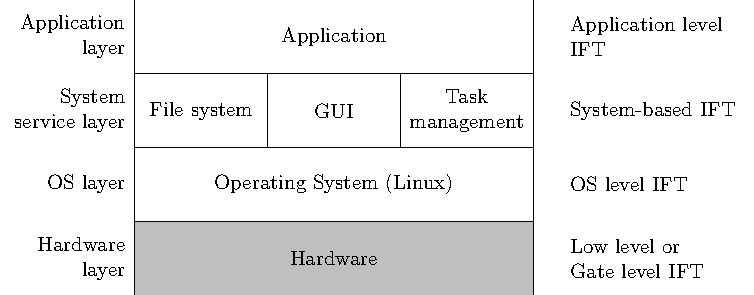
\includegraphics{c2_soa/img/system_layer.pdf}
    \caption{Simplified representation of the different layers in an embedded system}
    \label{fig:levels_system}
\end{figure}

Tracking information can be performed at various levels, from the application level to the hardware level. Each level offers distinct advantages and disadvantages.
For instance, application-level tracking might provide detailed insights and user-friendly interfaces, while hardware-level tracking offers more granular data and real-time monitoring but can be more complex and costly.
The following subsections explore these different levels, highlighting their respective benefits and limitations.


\subsubsection{Software-based DIFT}
\paragraph{Application level DIFT} tracks information flows between application variables. The programmer has to integrate data tagging inside his program and use a modified compiler or analyse his program to check if no security violation happened.
One application for DIFT at application level is language-based. Several security extensions have been proposed for existing programming languages.
JFlow~\cite{M-99-popl} is one of the first works that has described an extension of the Java language by adding statically-checked information flow annotations.

Multiples works introduce DIFT extensions for different languages, for example, such as JavaScript~\cite{CN-15-ccs, AF-09-plas}.
Austin et al.~\cite{AF-09-plas} propose a method for tracking information flow in dynamically-typed languages, focusing on addressing issues with implicit paths through a dynamic check. This approach avoids the necessity for approximate static analyses while still ensuring non-interference. The method employs sparse information labelling, keeping flow labels implicit where possible and introducing explicit labels only for values crossing security domains.

Kemerlis et al.~\cite{KPJK-12-sigplan} provide a framework, \textit{libdft}, which is fast and reusable and applicable to software and hardware. \textit{libdft} provides an API for building DFT-enabled tools that work on unmodified binaries.

\paragraph{OS level and System-based DIFT} track and tag files (read or written) used by the application.
The main advantage of this approach is that it reduces the number of information flows, which lead to an improvement of the runtime overhead. In the other side, the main disadvantage of this approach is that it results in more false positives than the application-level approach.

TaintDroid~\cite{EGHTCCJMS-14-tocs} introduces an extension to the Android mobile phone platform designed to monitor the flow of privacy-sensitive data through third-party applications. Operating under the assumption that downloaded third-party applications are untrusted, TaintDroid tracks in real-time how these applications access and handle users’ personal information. The primary objectives are to detect when sensitive data is transmitted out of the system by untrusted applications, and to enable phone users or external security services to analyse these applications. They store the data adjacent to data for spatial locality. This may cause large performance and storage overheads, as the tag fetching requires extra clock cycles for memory access.
HiStar~\cite{ZBKM-11-commacm} is a new OS that has been designed to provide precise data specific security policies. The authors made the choice to assign tags to different objects in the operating system instead of data.


\subsubsection{Software and Hardware Co-Design-Based DIFT}
This type of design combines the features of both software DIFT and hardware DIFT. Using binary instrumentations and a modified compiler, the hardware and software co-design can provide the best of these two categories of DIFT: flexible security configuration and fine-grained protection with low impact on performances~\cite{CGDJ-21-micromac, BSMCVEJCO-21-acmcsur}.

One example of this type of DIFT is RIFLE~\cite{VBCROBRVA-04-micro}, a runtime information-flow security system designed from the user's perspective, provides a practical means to enforce information-flow security policies on all programs by leveraging architectural support.
RIFLE employs binary instrumentation and architectural support to enforce information flow security policies during runtime. The conventional Instruction Set Architecture (ISA) is transformed into an Information-Flow Security (IFS) ISA using a dedicated binary translator. Each instruction in the ISA corresponds to an instruction in the IFS ISA. 
In the IFS ISA, additional security registers are assigned to hold tags. To avoid the pitfalls dynamic mechanisms encountered while tracking implicit flows, the binary translation will convert all implicit flows to explicit flows. The RIFLE architecture is then responsible only for tracking explicit flows. The translated binary is executed within a modified processor supporting the IFS ISA, which is simulated within the Liberty Simulation Environment. RIFLE works with every programs that run on a system, and policy decisions are left to the user, not the programmer.

Townley et al.~\cite{TKPAY-19-micro} presented LATCH, a generalizable architecture for optimizing DIFT. 
LATCH exploits the observation that information flows under DIFT exhibit strong spatial and temporal locality, with typical applications manipulating sensitive data during limited phases of computation. The main objective is to detect attacks on the integrity of the system. The architecture consists of a software-assisted hardware accelerator (S-LATCH) running on a single simulated core. The software component of S-LATCH propagates tags, while the hardware accelerator monitors the data accessed by the program to detect tags. 

Porquet et al.~\cite{PS-13-codes} presented WHISK, a whole system DIFT architecture implemented within a hardware simulator. WHISK stores tags and data separately in memory locations to keep low area overhead and improve flexibility and to better accommodate the integration of hardware accelerators.. Tag insertion, storage, and access to the custom hardware are delegated. The software subsystem uses MutekH exokernel-based OS and provides support for tag page allocation, page table cache configuration, and interrupt handling concerning writes to untagged pages.


\subsubsection{Hardware-based DIFT}
Dalton et al.~\cite{DKK-07-sigarch} report that software DIFT solutions add significative runtime overhead, up to a slow-down of 37 times ! Therefore, in order to improve the execution time to be more on-the-fly, the idea is to directly implement the DIFT into the hardware, but the trade-off is flexibility.
This subsection discusses the hardware-based DIFT designs, including gate-level DIFT designs and micro-architecture-level DIFT designs. Surveys~\cite{HAK-21-acmcsur,BSMCVEJCO-21-acmcsur} present an overview on all hardware DIFT techniques. They developed a taxonomy for them and use it to classify and differentiate hardware DIFT tools and techniques.

\paragraph{Gate-Level DIFT} include gate-level netlist and also RTL designs. The goal is to protect against hardware trojans and unauthorized behaviours. To achieve that, during the creation of the circuit, additional logic is added for each gate used in the design.

GLIFT~\cite{TWMMCS-09-asplos} is a well-established IFT technique. The goal is to protect against hardware trojans and unauthorized behaviours. All information flows, both explicit and implicit, are unified at the gate level. GLIFT employs a detailed initialisation and propagation policy to precisely track each bit of information flow, by adding additional logic for each gate used in the design. By analysing how inputs influence outputs, GLIFT accurately measures true information flows and substantially reduces the false positives typically associated with conservative IFT techniques.
Hu et al.~\cite{HOITSMK-11-tcad} established the theoretical foundation for GLIFT. They introduced several algorithms for generating GLIFT logic in large digital circuits. Additionally, the authors identified the primary source of precision discrepancies in GLIFT logic produced by various methods as static logic hazards or variable correlation due to reconvergent fan-outs. Many other works have been done on GLIFT to attempt a decrease of the logic complexity.

\paragraph{Off-Core DIFT} operations are performed on a dedicated coprocessor working in parallel of the main core.
The main drawback is that this approach needs a support from the OS for the synchronisation between data computations and tags computations in order to stall one core if it needs to wait the other. But on the other hand, its advantage is that it does not require internal hardware modifications to the main kernel. Processor manufacturers do not prioritise this type of security, and as most processors are not open to the public, it is difficult to modify them.

Kannan et al.~\cite{KDK-09-dsn} described one of the first work using a coprocessor to improve tag computation runtime overhead. Traditional hardware DIFT systems require significant modifications to the processor pipeline, which increases complexity and design time. Figure~\ref{fig:offcore_dift} represent how an off-core DIFT would be implemented. Kannan et al. uses this idea for implementing their solution of DIFT.
This coprocessor handles all DIFT functionalities, synchronizing with the main processor only during system calls. This design eliminates the need for changes to the processor's pipeline, logic, or caches, making it more attractive. The coprocessor is small, with an area footprint of about 8\% of a simple RISC core, and introduces less than 1\% runtime overhead for SPECint2000 applications benchmark. The paper demonstrates that the coprocessor provides the same security guarantees as integrated DIFT architectures, supporting multiple security policies and protecting various memory regions and binary types. This approach offers a balanced solution in terms of performance, cost, complexity, and practicality compared to existing DIFT implementations.

\begin{figure}[ht]
    \centering
    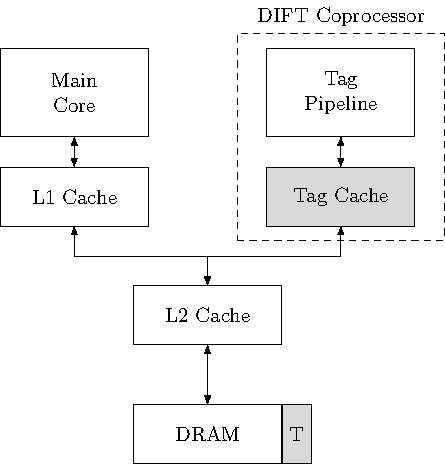
\includegraphics{c2_soa/img/offcore.pdf}
    \caption{Representation of a Hardware Off-Core DIFT (inspired by Figure 1 of~\cite{KDK-09-dsn})}
    \label{fig:offcore_dift}
\end{figure}

Wahab et al.~\cite{WCAHBLG-18-reconfig,WCAHLG-17-fpl} developed a DIFT using the ARM CoreSight debug component to extract a trace.
However, the debug component could only extract limited information about the application executing on the core. Therefore, some instrumentations have been required to recover the complete program trace. The information obtained from the trace is then sent to a dedicated DIFT coprocessor, which analyses the instruction trace and propagates tags according to a security policy. In terms of performance and area footprint, \cite{WCAHLG-17-fpl} gives around 5\% communication overhead and an area overhead of 0.47\% and a power consumption increased by 16\%; while~\cite{WCAHBLG-18-reconfig} gives a communication overhead of 335\%, an area increased by 0.95\% and a power consumption increased by 16.2\%. These results can not be compared to the initial design, as they use a coprocessor without the ARM core results.

\paragraph{Off-Loading DIFT} use a dedicated core of a multicore CPU~\cite{CKSFGMRRRV-08-sigarch,VHYR-08-cca,RGMRCKR-08-spaa}. Figure~\ref{fig:offloading_dift} represents how Off-Loading DIFT works with a core running the application and another, in parallel, run the DIFT analysis on the application trace. The application core is modified to create a trace and compress it. The trace includes executed instructions and packs main information such as PC address, register operands. This trace is then sent to the DIFT core via the L2 cache. Finally, the security core will decompress the trace and realizes tag computation in order to check whether an illegal information flow has been done. The notion of illegal information flow is specified thanks to a DIFT security policy.
The main advantage is that hardware does not need to know DIFT tags or policies and does not need a coprocessor with the management of the synchronisation between the two processors.  But the main drawback is that it requires a multicore CPU but reduces the number of core available and doubles the energy consumption due to the application trace analysis. In an embedded system where consumption is a critical factor, this solution is difficult to consider.

\begin{figure}[ht]
    \centering
    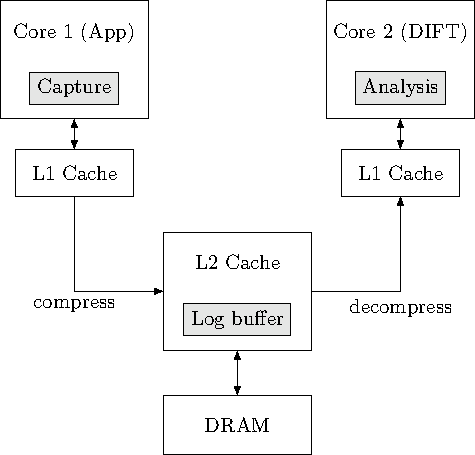
\includegraphics{c2_soa/img/offloading.pdf}
    \caption{Representation of a Hardware Off-Loading DIFT (inspired by Figure 1 of~\cite{KDK-09-dsn})}
    \label{fig:offloading_dift}
\end{figure}

\paragraph{In-Core DIFT} rely on a deeply modified processor pipeline which need to integrate tag computations inside the main core in parallel of data computations. This approach is highly invasive, but does not require any additional cores or coprocessors to operate and introduces no overhead for intercore synchronisation. Overall, its performance impact in terms of clock cycles over native execution is minimal. On the other hand, the integrated approach requires significant modifications to the processor core. All pipeline stages must be modified to add tags, a dedicated register file and first level of caches must be added to store tags in parallel with the regular blocks into the processor core. Figure~\ref{fig:incore_dift} shows the architecture of an In-Core hardware DIFT. When the processor fetches an instruction, its associated tag is sent in parallel. In the decode stage, the instruction is decoded while the security decode module decode the security policy to determine how the tag should be propagated and checked. When the instruction is executed, the tag is sent to a tag ALU to be checked. Then, if the tag is conforming to the security policy, the tag and the ALU output will be saved into the Data-Cache to be used again or stored in memory. Otherwise, if the tag is not conforming, the DIFT mechanism detects the security violation and can raise an exception, stop the application, depending on what is configured.

\begin{figure}[ht]
    \centering
    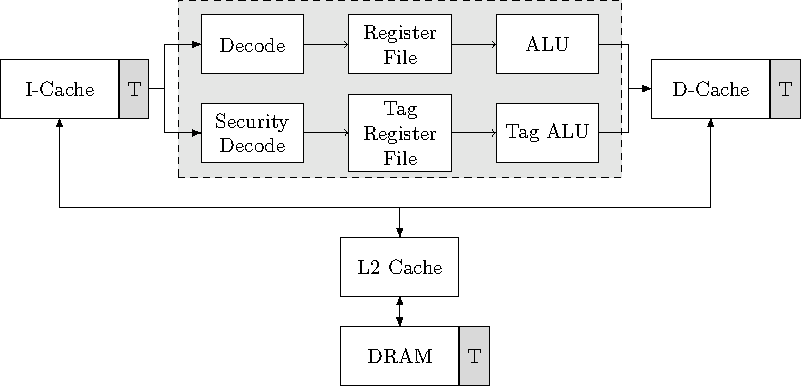
\includegraphics{c2_soa/img/incore.pdf}
    \caption{Representation of a Hardware In-Core DIFT (inspired by Figure 1 of~\cite{KDK-09-dsn})}
    \label{fig:incore_dift}
\end{figure}

Suh et al.~\cite{SLD-04-sigplan} proposed an approach in which the OS identifies a set of input channels as spurious, and the processor tracks all information flows from these inputs. Thanks to this tracking, the processor can detect various attacks such as attack targetting instructions or jump addresses. If the security policy detects something malicious in hardware, the OS will process the exception. They use a 1-bit tag, which means only two ways of representing security levels. They present two security policies that track differing sets of dependencies. Implementing the first policy incurs, on average, a memory overhead of 0.26\% and a performance decrease of 0.02\%. The second policy incurs, on average, a memory overhead of 4.48\% and a performance decrease of 0.8\%, and requires binary annotation unlike the first policy.

Dalton et al.\cite{DKK-07-sigarch} presented a DIFT architecture, Raksha, to support a flexible security configuration at runtime. They extended all storage locations including registers, caches and main memory with tags, they modified the ISA instruction to propagate and check tags. In this solution, they use 4-bits tags for each word. These tags represent the security policy and not the data state (e.g. trusted or untrusted). The authors provided two global sets of configuration registers, i.e., Tag Propagation Registers (TPR) and Tag Check Registers (TCR), to configure the security policy at runtime. There is one pair of TPR/TCR for each of the four security policies. The configuration register could be configured only in trusted mode. Moreover, the tag propagation and check could only be disabled in trusted mode. However, the security policy is difficult to update when the architecture is deployed.
The Raksha prototype is based on the Leon SPARC V8 processor, a 32-bit open-source synthesizable core, and they mapped the design onto an FPGA board.

Palmiero et al.~\cite{PDGLC-18-hpec} implemented a DIFT framework, D-RI5CY, on a RISC-V processor and synthesized it on a Field Programmable Gate Array (FPGA) board with a focus on IoT applications. The proposed design tags every word in data memory with a 4-bits tag and every general register with a 1-bit tag. Similarly to~\cite{DKK-07-sigarch}, Palmiero et al.~\cite{PDGLC-18-hpec} also adopted global configuration registers to customise the rule of tag propagation and checking. Each type of instruction has its own rule and can be modified separately. This method provides a more fine-grain tracking than Raksha but lacks flexibility for security policy reconfiguration for different program contexts.

%%%%%%%%%%%%%%%%%%%%%%%%%%%%%%%%
\subsection{How hardware DIFT work}
DIFT is a technique used in computer security to monitor the flow of information through a system. It aims to prevent security breaches such as data leaks, unauthorised data manipulation, and execution of untrusted code. In DIFT, each data is associated with a tag that indicates its security level.
For example, a tag might indicate whether data is 'trusted' or 'untrusted'. When data is input into the system, it is initially tagged based on its source.

As data moves through the system, these tags are tracked to ensure compliance with security policies and to ensure that sensitive information does not get exposed or manipulated improperly. For instance, if an operation involves both trusted and untrusted data, the result might be tagged as untrusted to ensure security.

An example of such security policy can be represented in Table~\ref{table:security_policies}. In this example, if the data comes from the network or if it's manipulated by a user, in the case of a \verb|scanf()| function in C language for example, the data cannot be trusted, while if the data comes from a secure channel or is manipulated by the system itself, the data can be trusted.

\begin{table}[ht]
    \centering
    \caption{Security policies for different data inputs}
    \label{table:security_policies}
    \begin{tabular}{@{}rcc@{}}
        \toprule
        \textbf{Data Input} & \textbf{Security Policy} & \textbf{Tag}     \\ \midrule
        User Input          & User-provided            & Untrusted        \\ \hline
        Network             & External source          & Untrusted        \\ \hline
        Internal            & System-provided          & Trusted          \\
        \bottomrule
    \end{tabular}
\end{table}

Figure~\ref{fig:dift_init} illustrates the three main steps of how DIFT works. Firstly, three data, $C_1$, $C_2$, and $C_3$, with their associated tags in three different colours, are initialised on the left side of the figure.

In the second step, when the data is fetched by the core for computation, the associated tags are propagated inside the core and confronted with the propagation policy depending on the operations performed on the data.

Finally, in the last step, on the right side of the figure, there are two data outputs derived from the three initial data. Data $C_4$ results from the combination of data $C_2$ and $C_3$, while data $C_5$ is derived from data $C_1$. Since data $C_1$ has not been modified, its tag remains the same. However, the tag associated with $C_4$ is a mix of tags from $C_2$ and $C_3$. Depending on the security policy, if $C_2$ was trusted and $C_3$ was not, the output tag will be \textit{untrusted}. Consequently, when the tags go through the final step of DIFT, they will be checked, and an exception may be raised or the application may be stopped due to the mixing of \textit{trusted} and \textit{untrusted} values.

\begin{figure}[ht]
    \centering
    \includegraphics[page=3]{c2_soa/img/schemaDIFT.pdf}
    \caption{Representation of the DIFT mechanism from initialisation to checking.}
    \label{fig:dift_init}
\end{figure}

%%%%%%%%%%%%%%%%%%%%%%%%%%%%%%%%%%%%%%%%%%%%%%%%%%%%%%%%%%%%%%%%%%%%%%%%%%%%%%%%%%%%%%%%%%%%%%%
\section{Physical Attacks}
\label{section:physicalAttacks}

This section presents an overview of the state of the art on physical attacks. We present the different types of physical attacks and their methods to recover secret information. Firstly, we begin with Side-Channel Attacks, how to use information leakage to recover useful information and how to analyse them.
Secondly, we introduce Fault Injection Attacks. We define the different possibilities of injection and how to achieve them.

Physical attacks are separated into two main categories: passive attacks and active attacks. Passive attacks are also called Side-Channel Attacks (SCA), and active attacks are often called Fault Injection Attacks (FIA). Figure~\ref{fig:arbo_fia} shows a representation of a taxonomy to classify the different method of physical attacks. Each type of attacks will be explained in this following subsections.

\begin{figure}[ht]
    \centering
    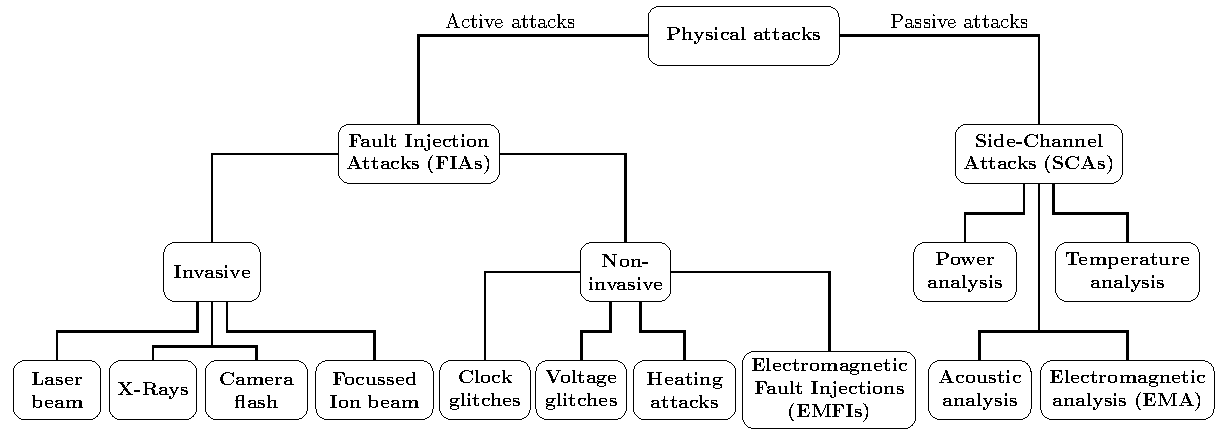
\includegraphics[width=\textwidth, page=1]{c2_soa/img/physicalAttacks.pdf}
    \caption{Taxonomy of the different methods of physical attacks (inspired by~\cite{CKNDCTD-21-compsec})}
    \label{fig:arbo_fia}
\end{figure}

\subsection{Side-Channel Attacks}
Side-Channel Attacks exploit information leakages on the circuit behaviour such as power consumption, electromagnetic radiation or the execution time of an application.
This type of attack does not call into question the theoretical integrity of the implementation, but aims to recover information by devious means. During data processing, the alternation between different states requires time and minimal energy dissipation, the variations of which can be analysed by the attacker.
This information allows the attacker to access secret data such as a password, or cryptographic key. The origin of these attacks date back to the \mbox{TEMPEST} program from NSA~\cite{F-72-nsa}. They described the vulnerabilities of a cryptographic implementation from their electromagnetic emissions, depending on the input and data.

Figure~\ref{fig:sca} represents the different methods of SCA on a microprocessor. We will go into detail of these different methods in the following text. The main idea is to have an application running on the processor and an attacker will use one method to trace the application multiple times to recover secret information (e.g. cryptographic key, password, private data, etc.).

\begin{figure}[ht]
    \centering
    \includegraphics[page=3, width=.75\textwidth]{c2_soa/img/physicalAttacks.pdf}
    \caption{Representation of the different methods of Side-Channel attacks}
    \label{fig:sca}
\end{figure}

\paragraph{Power analysis} exploits time differences in target power consumption during sensitive executions. Modern systems contain billions of transistors (up to 146 billions transistors for an AMD CPU Instinct MI300A\footnote{\url{https://www.amd.com/en/products/accelerators/instinct/mi300/mi300a.html}} or up to 208 billions transistors for a Nvidia GPU GB200 Grace Blackwell\footnote{\url{https://nvidianews.nvidia.com/news/nvidia-blackwell-platform-arrives-to-power-a-new-era-of-computing}}). These transistors act as voltage switches and as they are continually switched on/off during execution, they cause voltage variations that can be observed and measured using equipments and devices (oscilloscope, voltmeter, etc.). These results data are analysed and from a certain number of data, an attacker can deduce secrets.
Kocher et al.~\cite{KJJ-98-crypto,KJJR-11-jce} introduced this method of SCA to recover cryptographic key from the analysis of power consumption. They introduced the Simple Power Analysis method (SPA) and Differential Power Analysis (DPA)~\cite{GP-99-ches}. While SPA attacks mainly use visual inspection to identify relevant power variations, DPA attacks use statistical analysis and error correction techniques to extract information correlated to secret keys.
Lipp et al.~\cite{LKOSECG-21-sp} present an attack, PLATYPUS, a software-based power side-channel attack on Intel server, desktop, and laptop CPU. They exploit unprivileged access to the Intel Running Average Power Limit (RAPL) interface. By observing variations in power consumption, they achieve to monitor the control flow of applications and also infer data and extract cryptographic keys.

\paragraph{Execution time analysis} also known as timing attacks and first introduced by Kocher~\cite{K-96-crypto}, takes advantage of the fact that some sensitive computational operations vary in time depending on their secret inputs. An attacker can learn information about these inputs by measuring the running time of the operation. Inherently, these attacks require the attacker to obtain responses from the target to measure its runtime. The works of Kocher~\cite{K-96-crypto}, Brumley and Boneh~\cite{DD-05-compnet} demonstrate attacks on many popular cryptosystems, including DSS, RSA, and OpenSSL.

\paragraph{Electromagnetic analysis} exploits electromagnetic (EM) emissions signatures produced when conducting logic operations. Thus, EM emissions reflect the operations of the system. In 2001, Quisquater and Samyde~\cite{QS-01-scps} extended SCA with EM analysis.
EM SCA methods can be divided into Simple EM Attack (SEMA) and Differential EM Attack (DEMA) similarly to power attacks~\cite{ANM-19-di}. By observing different signal patterns of collected traces, SEMA can directly interpret cryptographic operations. DEMA extracts secret keys by comparing collected EM traces to hypothesised values and looking for peaks indicative of an accurate prediction~\cite{HGTVJ-22-dt}.
The attacker collects EM radiation using an EM probe. The probe is placed near the electronic equipment. At this stage, the quality of the collected EM traces, and thus the effectiveness of EM SCA, is strongly affected by several measurement parameters such as EM probe, noise, trigger, sampling rate and frequency band. Recent work has shown that different EM probe characteristics (e.g. diameter, orientation) and spatial location significantly affect EM traces~\cite{HMHSS-12-tcrypo,KSTO-17-iccad, WDL-16-ntms}.

\paragraph{Temperature analysis} exploit the temperature values induced by the activity of the system. This attack is linked to electromagnetic and power analysis, as they use traces from the system's execution. Aljuffri et al.~\cite{AZRHT-21-tvlsi} presented a study on thermal analysis where three different power-based SCAs were modified for thermal attacks and applied to a naive RSA implementation. Their experiments were able to retrieve the secret key with an accuracy of 100\%. Another experiment attacked a protected implementation of RSA and completed the extraction of the key with only five traces. Hutter et al.~\cite{HS-14-cardis} present results of data leakages of CMOS devices from temperature SCA. They study the leakage of processed data by measuring the dissipated heat of the devices.

\paragraph{Acoustic analysis} takes advantage of the analysis of the sound emitted by the systems. This technology has been around for a long time and is used in many fields, such as sonar. The "golden ear" in a submarine listens to the sounds of the sea and is able to detect and distinguish a submarine, a warship, or a merchant vessel by the sound of its turbine alone. It is also able to determine its direction and nationality.

Computers emit high-pitched sounds when they are running. This is due to vibrations in some of their electronic components. These sounds are more than just a nuisance. They can convey information about the software running on the computer. In particular, they can reveal sensitive information about security-related calculations. People have shown that it is possible to recover RSA keys from their sound.
Backes et al.~\cite{BDGPS-10-usenix} present an attack that retrieves what a dot-matrix printer is printing from a recording of the sound it makes. Their experiments show that they can recover up to 72\% of the words printed, and up to 95\% if they know the context of the text. For this experiment, they used a dictionary-based approach to printed English words.
Genkin et al.~\cite{GST-17-crypto} demonstrated that RSA key extraction using acoustic cryptanalysis was feasible against a Lenovo laptop from a smartphone nearby. The authors targeted GnuPG's RSA implementation using a laboratory microphone setup and a Samsung Note II, and showed that a 4096-bit key could be recovered within an hour using audible and ultrasonic sound emanations. Harrison et al.~\cite{HTM-23-eurospw} present an implementation of a deep-learning model to classify laptop keystrokes using a microphone. They use the trained model to recognise the keystrokes, and they achieve an accuracy of 95\%. They trained their model from a Zoom conference and this time they achieve an accuracy of 93\%. Their results have shown that it is possible to recover password or other secret information of a victim from its keystrokes even without a physical presence.

\subsection{Fault Injection Attacks}
As early as the 1970s, with advances in the space industry, anomalies in the operation of electronic circuits were observed and possibly linked to cosmic radiation outside the Earth's atmosphere~\cite{BSH-75-tns,Z-96-ibm,ZL-79-science}. These disturbances were initially found to affect the performance of electronic systems in space environments, where high-energy particles could disrupt the normal functioning of circuits. However, as transistors became smaller and required less energy to operate, similar phenomena were observed in terrestrial environments and aircraft systems. These transient disturbances, commonly referred to as "\textit{soft errors}", are now recognised as a critical issue in both space and ground electronics, affecting everything from memory chips to complex processors.

However, in addition to these induces cosmic faults, wanted faults exist and are known as Fault Injection Attacks (FIA). FIA involves deliberately introducing a fault into the system to observe its behaviour and identify potential vulnerabilities. If the error caused by the fault does not propagate and execution of the application completes normally, the fault is ineffective. On the other hand, if the fault affects the execution of the application, causing it to fail or behave differently than expected, then the fault is effective. These faults can impact the performance, functionality, and reliability of the circuit. These attacks can induce errors in internal electronic components, which can be utilised to recover cryptographic keys and other secret data.
These attacks have been vastly studied since the first introduction of these attacks by Boneh et al. in 1997~\cite{BDL-97-eurocrypt,BDL-01-crypto}. Multiple studies or surveys~\cite{ZAV-06-jarab, BCNTW-06-procieee, CKNDCTD-21-compsec, PBR-15-dtis, YSW-18-hss, BH-22-access} present the different sources of FIA.
Figure~\ref{fig:fia} presents a summary of the different methods of FIA, the figure does not represent all possible methods. Each of these attacks requires equipment which is more or less expensive and easy to acquire, ranging from a few hundred euros (clock glitches, voltage glitches) to several hundred thousand (Laser, X-Ray, Focused Ion Beam).

As shown in the Figure~\ref{fig:arbo_fia}, these attacks are categorised as transient or permanent, and invasive or non-invasive.
The effect of a transient fault lasts for a limited period of time. These faults rarely do any lasting damage to the component affected, although they can induce an erroneous state in the system. Their aim is to temporarily disrupt the program control flow or corrupt the results of an instruction to gain unauthorised access to sensitive code and data.
By opposition, permanent faults or destructive faults, created by purposely inflicted defects to the chip’s structure, have a permanent effect. Once inflicted, such destructions will affect the chip’s behaviour permanently and persist irrespective of device restarts and resets.

Invasive attacks involve major alteration to the Device Under Test (DUT), such as decapping the System-on-Chip (SoC) to expose its internals and remove any protective layers. These processes risk irreparable damage or destruction of the target under evaluation, potentially leading to permanent data loss.

Non-invasive attacks require no tampering of the DUT. They are able to mask their presence as they have no effect on the system other than the faults they inject.

\begin{figure}[ht]
    \centering
    \includegraphics[page=2, width=.75\textwidth]{c2_soa/img/physicalAttacks.pdf}
    \caption{Representation of the different methods of Fault Injection attacks}
    \label{fig:fia}
\end{figure}

\subsubsection{Invasive attacks}
Invasive attacks need to decapsulate the chip or the Integrated Circuit (IC).
Decapsulating a die or integrated circuit (IC) is a process used to expose the internal components of an IC, typically for failure analysis or reverse engineering. The goal is to carefully remove the protective encapsulation, which shields the silicon die and is typically made of epoxy or ceramic, without causing damage to the internal structures. There are several methods to achieve this, each suited to different packaging materials and levels of precision, ranging from chemical processes to advanced techniques like laser ablation and plasma etching.

The most common method is chemical decapsulation, which involves etching away the epoxy with concentrated acids such as nitric or sulphuric acid. This process requires safety precautions such as protective clothing and neutralisation of the acids after removal of the encapsulation. It is an effective but dangerous process and require careful control to avoid damaging the die, as over-etching can cause irreversible harm.

Another method is laser decapsulation, which uses a precision laser to remove the encapsulation material layer by layer. This technique is highly accurate and reduces the risk of damage to the die, but it is expensive and requires specialised equipment. Mechanical decapsulation involves physically grinding or cutting away the encapsulation, but has a high risk of damaging the die, especially when approaching the final layers.

Plasma etching is a more advanced technique that uses ionised gases to gradually etch away the encapsulation material. It offers high precision but is slower than other methods and is typically used in research or industrial environments. Whichever method is used, safety precautions are essential, especially when dealing with hazardous chemicals and sensitive materials.

Figure~\ref{fig:decapsulating_die} shows three different steps to decapsulate a circuit. To be noted, this processor is the AMD Zen2 EPYC 7702 server processor which is not for embedded systems.

\begin{figure}[ht]
    \centering
    \begin{subfigure}[b]{0.3\textwidth}
        
\includegraphics[width=\textwidth]{c2_soa/img/epyc_7702_initial.jpg}
        \caption{Initial die from an AMD Zen 2 EPYC 7702 server processor}
        \label{fig:initial_die}
    \end{subfigure}
    \hfill
    \begin{subfigure}[b]{0.3\textwidth}
        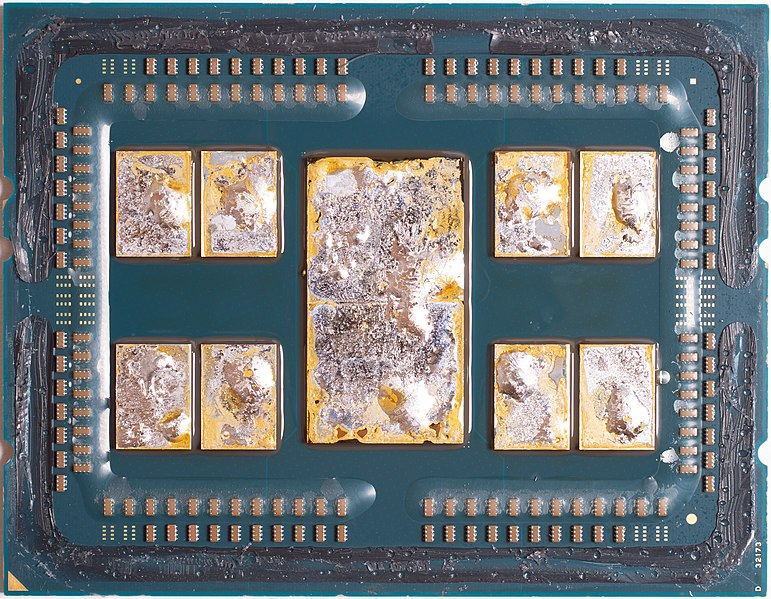
\includegraphics[width=\textwidth]{c2_soa/img/epyc_7702_delidding.jpg}
        \caption{AMD EPYC 7702 after delidding, with remains of solder thermal interface material (TIM)}
        \label{fig:delidding_die}
    \end{subfigure}
    \hfill
    \begin{subfigure}[b]{0.3\textwidth}
        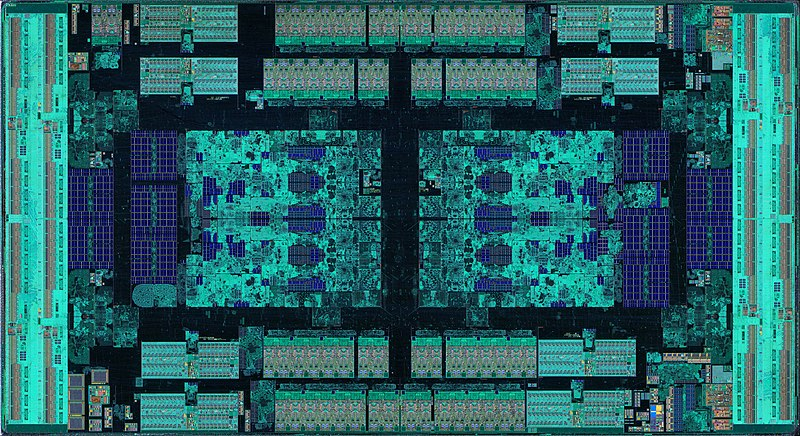
\includegraphics[width=\textwidth]{c2_soa/img/epyc_7702_packagedRemoved.jpg}
        \caption{Die shot of the center die, after removal from processor package substrate and metallization etching}
        \label{fig:packagedRemoved_die}
    \end{subfigure}
    \caption{Three steps to decapsulate a die (from~\cite{decapping-19-wikipedia})}
    \label{fig:decapsulating_die}
\end{figure}


\paragraph{Camera flash/light source} is a type of optical attack. The attacker needs to decapsulate the chip, and the strong radiation emitted by the flash directed at the silicon surface can cause the blanking of memory cells where constant values are stored for algorithms execution (e.g., the AES S-Boxes). These attacks are inexpensive, but, in the other hand, they are not very accurate. Skorobogatov et al.~\cite{SA-02-ches} used a flashgun for \$30 while being able to change any bit of an SRAM array.

Schmidt and Hutter~\cite{SH-07-austrochip} present practical attacks on implementations of RSA that use Chinese Remainder Theorem (CRT). These attacks have been performed into a cryptographic device through optical and EM injections. They use a laser diode  as a light source, the diode emitts a light  beam of \SI{100}{\milli\watt} with a wavelength of \SI{785}{\nano\metre}. The light from the diode is guided thanks to a fibre-optic of 1~mm in diameter.

Guillen et al.~\cite{GGD-17-cosade} present a low-cost fault injection setup, around couple hundred euros, which is capable of producing localized faults in modern 8-bit and 32-bit microcontrollers. This setup does not require handling dangerous substances or wearing protection equipment. The fault produced by this setup are able to successfully attack real-world cryptographic implementations, such as the NSA’s Speck lightweight block cipher~\cite{RDJSBL-13-nsa}.

\paragraph{Laser beam} is another type of optical attacks.
The injected fault is similar to the one used with a camera flash, with the exception of which is a lot more precise and is capable of always inducing faults.
The main downside of this method is that it requires a high expertise.
Dutertre et al.~\cite{DBCDFFGHLMDPR-18-fdtc} explain the theory behind this technique at the lowest level.

Figure~\ref{fig:ls2} shows an example of a laser fault injection station made by Riscure.
It contains powerful red and NIR diode lasers (resp.\SI{14}{\watt}, and \SI{20}{\watt}). The red laser is designed for frontside testing of smart card chips and in combination with the optics it produces a spot size of 6 * \SI{1.4}{\micro\metre} on the chip surface. The near-infrared laser is designed for backside testing of smart card chips. This powerful diode laser penetrates the chip substrate to reach the transistors.
This station automates the surface scanning process, offers precise control of laser power, and injects pulses with a small spot size. It has a precise and fast response thanks to a trigger and the ability to perform multi-glitching.

Using a laser beam, a single bit~\cite{CMDMRD-19-host} in a memory can be set (from logical 0 to logical 1) or reset (from logical 1 to logical 0) by attacking either front side or the back side of the chip.
Today, the capabilities of laser injection mechanisms make it possible to carry out attacks with multiple faults.
Colombier et al.~\cite{CGVCBLC-22-cardis} use a four-spot laser bench to inject up to 4 non-contiguous bits in a single cycle, or multiple non-contiguous bits over multiple cycles. This fault injection mechanism therefore makes it possible to construct much more complex attacks, potentially capable of bypassing many countermeasures.

Breier et al.~\cite{JHJBC-17-hss} studied the fault mechanism of circuit logic elements in FPGA environment, and performed a practical laser fault injection into a single bit CED-protected block cipher in Xilinx Virtex-5 FPGA.
Figure~\ref{fig:lfi_setup} shows their setup to inject fault into a Xilinx Virtex-5 FPGA.
The chip is preprocessed by a mechanical solution in order to reduce the substrate thickness, to approximatively \SI{100}{\micro\metre}. Thinner substrate leads to easier laser penetration, at the risk of destroying logic resources or routing channels on the chip.
The laser used is a \SI{20}{\watt} diode pulse laser with 5 times magnification lens, which reduce the effective maximum power to \SI{10}{\watt}. The wavelength is \SI{1064}{\nano\metre} and the spot size of the laser beam is approximatively \SI{840}{\micro\metre}$^2$.

\begin{figure}[ht]
    \centering
    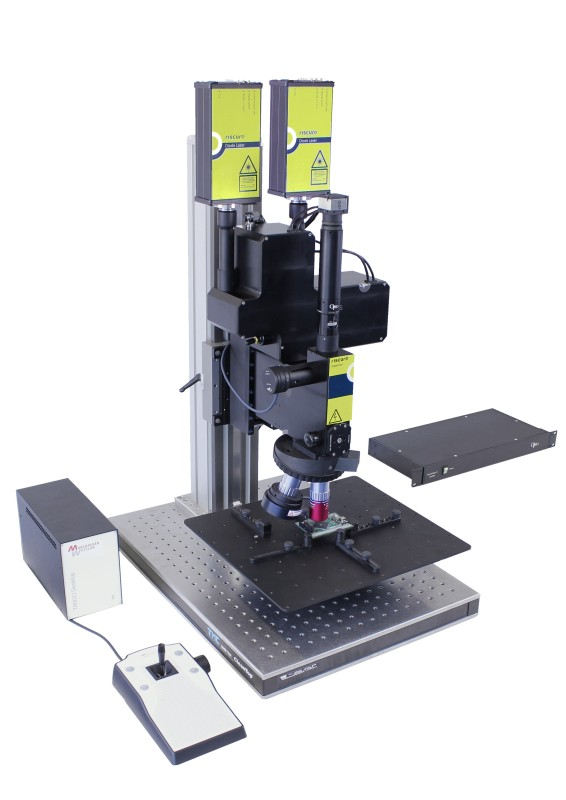
\includegraphics[width=0.5\textwidth]{c2_soa/img/LS2.jpeg}
    \caption{Example of a laser fault injection station (by Riscure Laser Station 2~\cite{riscure_station})}
    \label{fig:ls2}
\end{figure}

\begin{figure}[ht]
    \centering
    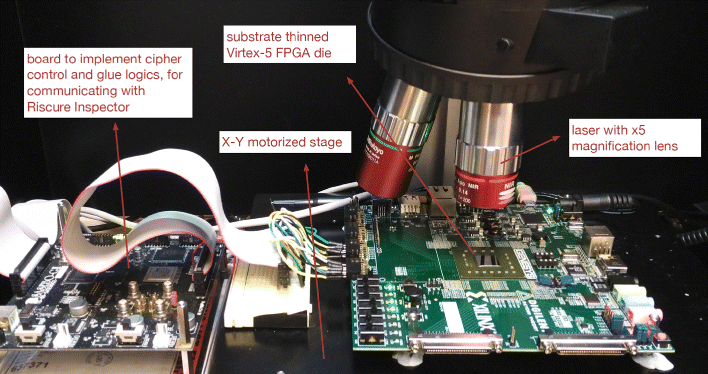
\includegraphics[width=\textwidth]{c2_soa/img/lfi_setup.png}
    \caption{Example of a laser fault injection setup (by~\cite{JHJBC-17-hss})}
    \label{fig:lfi_setup}
\end{figure}

\paragraph{Focused ion beam} is the most accurate and powerful fault injection technique used. Focused ion beam (FIB) enables an attacker to arbitrarily modify the structure of a circuit, reconstruct missing buses, cut existing wires and rebuild them.

FIB can operate at a precision of \SI{2.5}{\nano\metre}, which is the size of a transistors in actual IC. FIB workstations require very expensive consumables and a strong technical background to fully exploit their capabilities. The only limit to the FIB technology is the diameter of the atoms whose ions are used as a scalpel. Currently, the most common choice is Gallium, which sets the lower bound to roughly \SI{0.135}{\nano\metre}.

\cite{FVMBMWP-23-wfiot} \wip{vérifier que ça va ici}

\subsubsection{Non-invasive attacks}
Non-invasive attacks involve inducing errors in a system without physically tampering with the device. These attacks exploit external influences like electromagnetic interference, voltage glitches, or clock signal manipulation to cause faults during the device's operation. Unlike invasive methods, which require dismantling or altering the hardware, non-invasive techniques leave no physical traces, making them harder to detect. By injecting faults at precise moments, attackers can bypass security mechanisms, retrieve sensitive data, or alter the device's intended functionality.

\paragraph{X-Rays} is another approach to inject fault very precisely but this method is not invasive as X-Rays can go through the IC package without the need of decapsulating it. Another advantage is that X-Ray have a lot smaller wavelength, down to \SI{0.01}{\nano\meter}, than laser injection which are limited to the wavelength of their light source, down to \SI{1}{\micro\meter}.
The injected fault is semi-permanent, and to make it disappear, the attacker has to heat up the device. This differs from other techniques where the fault can disappear a few cycles after injection.
This technique can be compared as a non-invasive FIB techniques. X-ray provides many opportunities for attacking electronic circuits. Among them, we can note the possibility to cause permanent faults in cryptographic algorithms, deactivation of countermeasures, reprogramming of memories, etc.

Anceau et al.~\cite{ABCMRT-17-ches, BAMCST-23-dft} propose an approach for modifying the behaviour of a transistor in the memory of a circuit using focused X-ray beams. 
They use the European Synchrotron Radiation Facility (ESRF), in Grenoble, France.

Grandamne et al.~\cite{GBD-23-paine} show efficiency of X-Ray faults injection on flash and EEPROM memories for powered off devices. They also describe a fault model according to their experimental results and propose a solution to correct a part of the fault.

\paragraph{Clock glitches} \wip{à finir}

Figure~\ref{fig:clock_glitch} represent

\begin{figure}[ht]
    \centering
    \includegraphics[page=4]{c2_soa/img/physicalAttacks.pdf}
    \caption{Representation of a clock glitch attack}
    \label{fig:clock_glitch}
\end{figure}


\begin{figure}[ht]
    \centering
    \includegraphics[page=5]{c2_soa/img/physicalAttacks.pdf}
    \caption{Representation of the parameters of a clock glitch attack}
    \label{fig:clock_glitch_parameters}
\end{figure}

\paragraph{Voltage glitches}
\wip{insérer image / schéma voltage glitch}

\begin{figure}[ht]
    \centering
    \includegraphics[page=6, scale=1.25]{c2_soa/img/physicalAttacks.pdf}
    \caption{Representation of a voltage glitch attack}
    \label{fig:voltage_glitch}
\end{figure}


\paragraph{Heating attacks}

\paragraph{Electromagnetic fault injections (EMFI)}

\begin{figure}[ht]
    \centering
    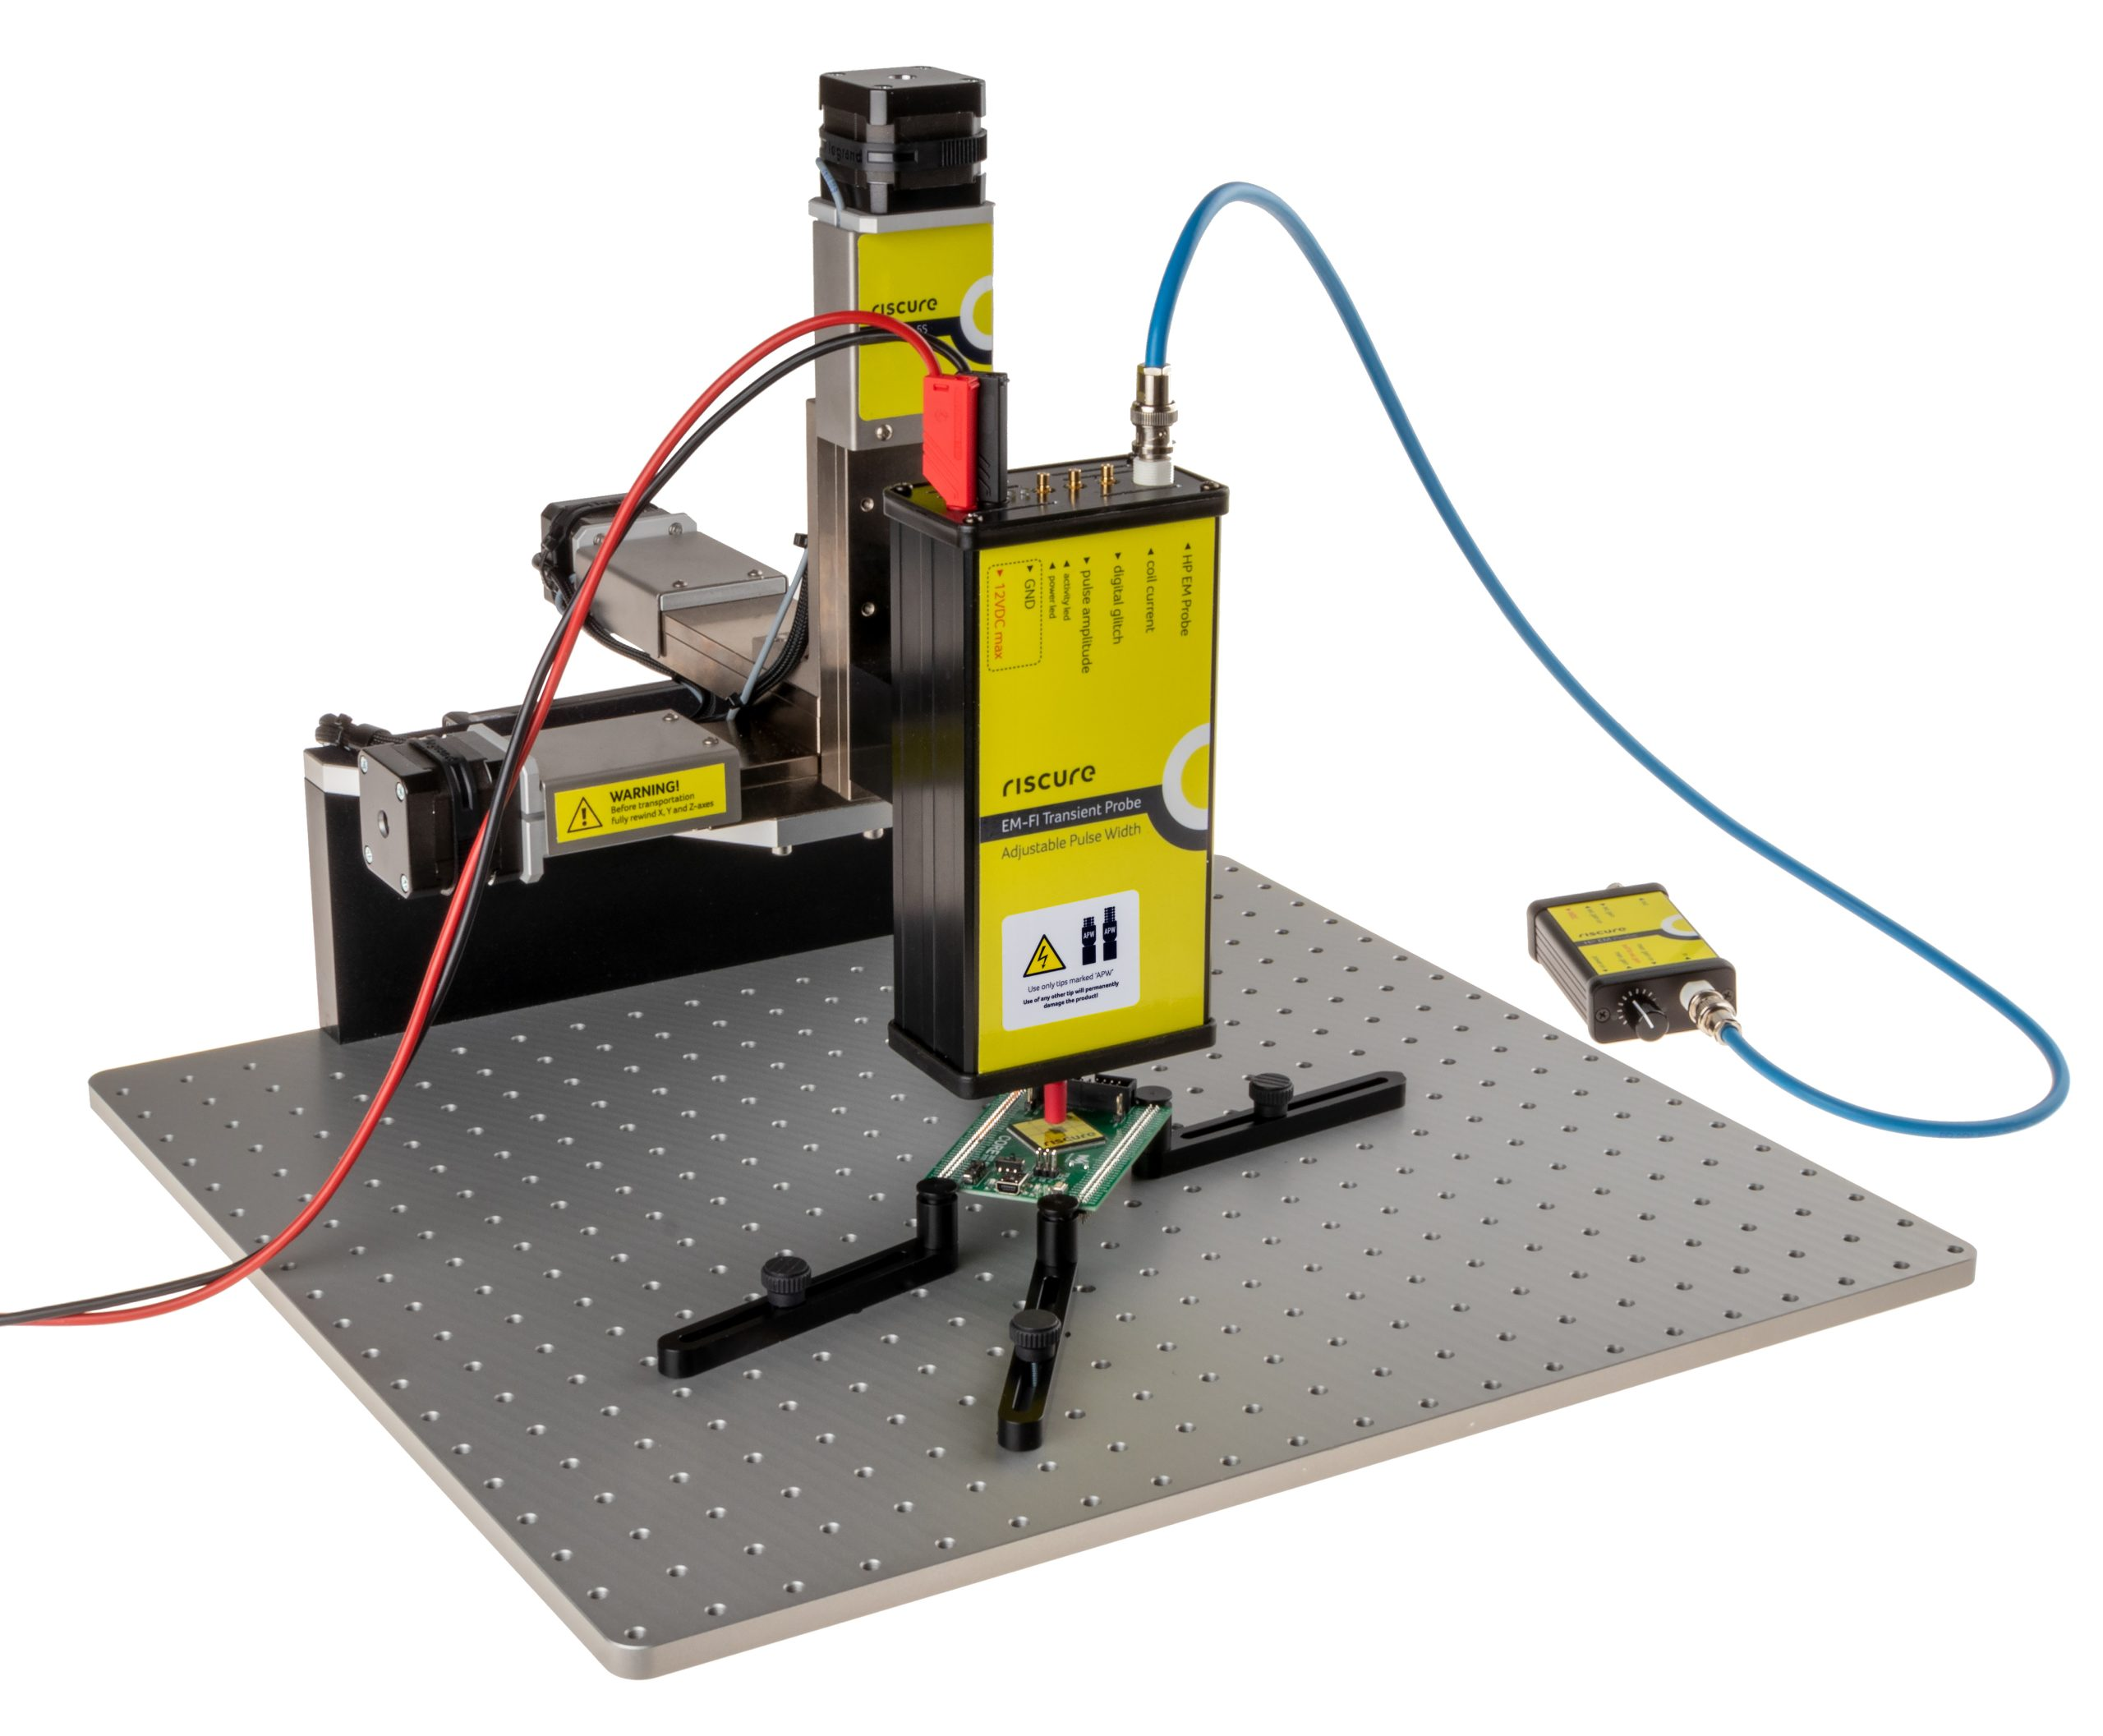
\includegraphics[width=.5\textwidth]{c2_soa/img/emfi_riscure_setup.jpg}
    \caption{Example of an EMFI attack setup}
    \label{fig:emfi_setup}
\end{figure}

\subsubsection{Summary}

\begin{table}[ht]
    \centering
    \caption{Fault Injection methods summary}
    \label{tab:fia_techniques}
    \begin{tabular}{@{}rccccc@{}}
        \toprule
        \textbf{Technique}        & \begin{tabular}{c}\textbf{Precision}\\{\small\textbf{(time)}}\end{tabular} & \begin{tabular}{c}\textbf{Space}\\\textbf{accuracy} \end{tabular}  & \textbf{Cost}              & \textbf{Expertise} & \begin{tabular}{c}\textbf{Damage}\\\textbf{risk} \end{tabular} \\ \midrule
        Clock Glitches   & High           & Low             & Low           & Low       & Very low      \\
        Voltage Glitches & Moderate       & Low             & Low           & Low       & Very low      \\
        Heating attacks  & Very low       & Very low        & Low           & Very low  & Moderate      \\
        Camera flash     & Moderate       & Low             & Moderate      & Moderate  & High          \\
        EMFI             & High           & High            & Moderate      & Moderate  & Low           \\
        Laser            & Very high      & Very high       & High          & High      & Very high     \\
        Focused Ion Beam & Very high      & Very high       & Very high     & Very high & Very high     \\
        X-Ray            & Very high      & Very high       & Highest       & Very high & Very low      \\
        \bottomrule
    \end{tabular}
\end{table}

\subsubsection{Fault models}

%%%%%%%%%%%%%%%%%%%%%%%%%%%%%%%%%%%%%%%%%%%%%%%%%%%%%%%%%%%%%%%%%%%%%%%%%%%%%%%%%%%%%%%%%%%%%%%
\section{Countermeasures against FIA}
\label{section:countermeasuresAgainstFIA}

%%%%%%%%%%%%%%%%%%%%%%%%%%%%%%%%%%%%%%%%%%%%%%%%%%%%%%%%%%%%%%%%%%%%%%%%%%%%%%%%%%%%%%%%%%%%%%%

\clearemptydoublepage
\chapter{D-RI5CY - Vulnerabilities Assessment}
\chaptermark{Dynamic Information Flow Tracking - Vulnerabilities Assessment}
\label{chapter:dift_assessment}
\minitoc

This chapter provides the background of this thesis and the vulnerability assessment. The first section offers a description of the RISC-V Instruction Set Architecture (ISA) and an overview of the specific RISC-V DIFT design under consideration.
The second section details and describes the considered uses cases of this thesis.
Finally, the third section assesses the vulnerabilities of the D-RI5CY, using these three cases.

%%%%%%%%%%%%%%%%%%%%%%%%%%%%%%%%%%%%%%%%%%%%%%%%%%%%%%%%%%%%%%%%%%%%%%%%%%%%%%%%%%%%%%%%%%%%%%%
\section{D-RI5CY}
\label{section:driscy}
In this section, we describe the RISC-V ISA and detail the DIFT design we have chosen to focus on.

\begin{figure}[t]
    \centering
    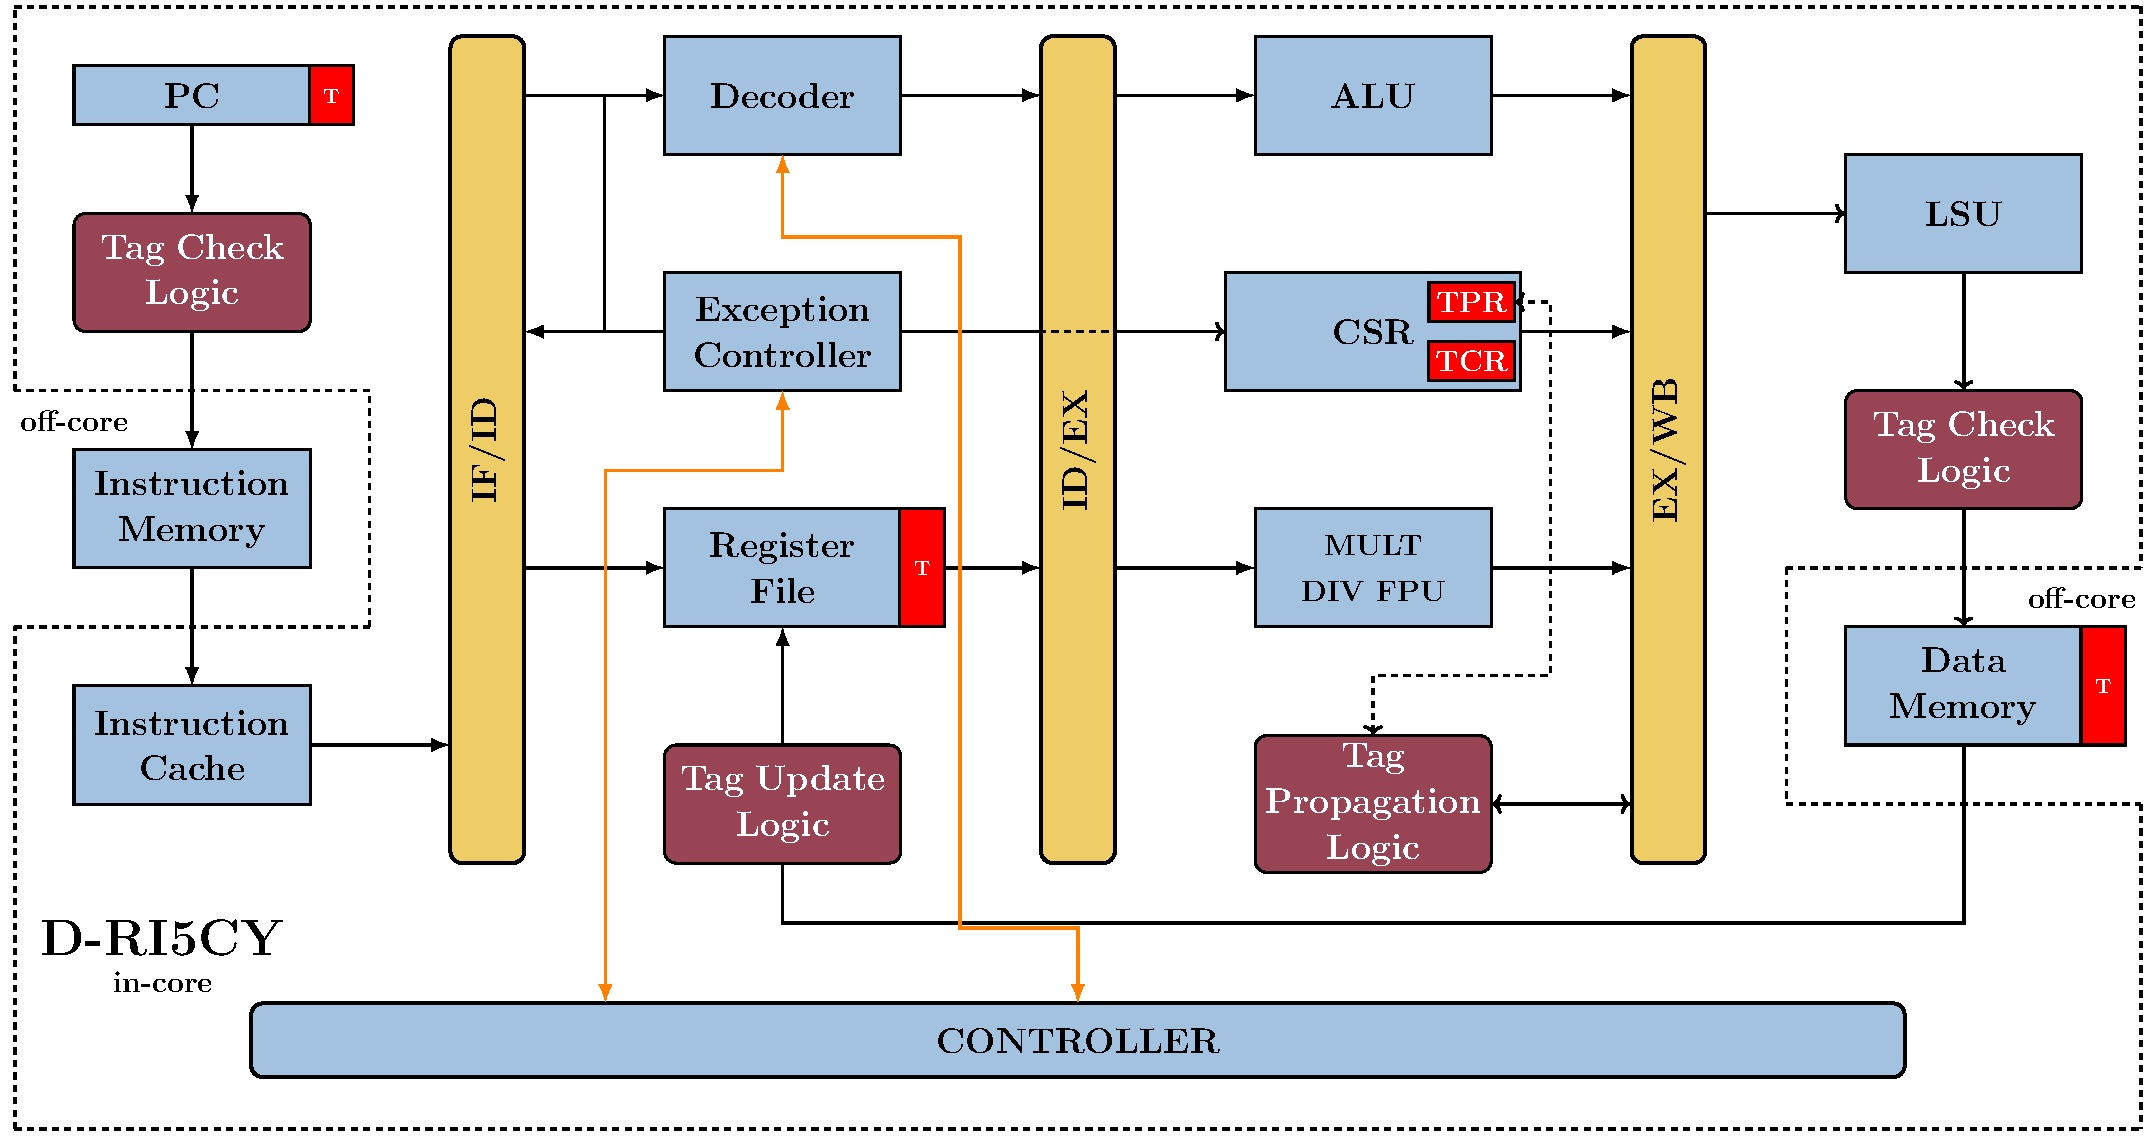
\includegraphics[width=\textwidth]{c3_vulnerabilities_assessment/img/RI5CY.pdf}
    \caption{D-RI5CY processor architecture overview. DIFT-related modules are highlighted in red.}
    \label{fig:driscy}
\end{figure}

%%%%%%%%%%%%%%%%%%%%%%%%%%%%%%%%
\subsection{RISC-V Instruction Set Architecture (ISA)}
RISC-V is an open and free ISA, which was originally developed at University of California, Berkeley, in 2010, and now is managed and supported by the RISC-V Foundation, having more than 70 members including companies such as Google, AMD, Intel, etc. The architecture was designed with a focus on simplicity and efficiency, embodying the Reduced Instruction Set Computer (RISC) principles. Unlike proprietary ISA, RISC-V is freely available for anyone to use without licensing fees, making it a popular choice for academic research, commercial products, and educational purposes.

Technically, RISC-V features a modular design, allowing developers to incorporate only the necessary components for their specific application, which can significantly reduce the processor's complexity and power consumption. It supports several base integer sets classified by width—mainly RV32I, RV64I, and RV128I for 32-bit, 64-bit, and 128-bit architectures respectively. Each base set can be extended with additional modules for applications requiring floating-point computations (e.g., RV32F, RV64F), atomic operations (e.g., RV32A, RV64A), and more. This modularity and the openness of RISC-V have spurred a wide range of innovations in processor design and applications in areas ranging from embedded systems to high-performance computing.

%%%%%%%%%%%%%%%%%%%%%%%%%%%%%%%%
\subsection{DIFT design}
For this thesis, we opted not to develop a Dynamic Information Flow Tracking (DIFT) system from the ground up, as this would have required considerable time for implementation and testing, which was not within the scope of our objectives. Consequently, we decided to review the current state of the art and select an open-source DIFT system.
As a result, we have selected the D-RI5CY~\cite{PDGLC-18-hpec, driscy} design, which utilises the RI5CY core supported by PULPino and developed by ETH Zurich. This is a 4-stage, in-order, 32-bit RISC-V core optimised for low-power embedded systems and IoT applications. It fully supports the base integer instruction set (RV32I), compressed instructions (RV32C), and the multiplication instruction set extension (RV32M) of the RISC-V ISA. Additionally, it includes a set of custom extensions (RV32XPulp) that support hardware loops, post-incrementing load and store instructions, and, ALU and MAC operations.

D-RI5CY has been developed by researchers of Columbia University, in the USA, in partnership with Politecnico di Torino, in Italy. D-RI5CY use the RI5CY processor, in which they implemented a hardware in-core DIFT.

Figure~\ref{fig:driscy} presents an overview of the D-RI5CY processor's architecture. In red and dark red are represented the DIFT specific modules.
These modules allow tags to be initialised, propagated and checked during the execution of a sensitive application.
The \textit{Tag Update Logic} module is used to initialize or update the tag in the register file according to the tagged data.
Then, when a tag is propagated in the pipeline in parallel to its associated data, the \textit{Tag Propagation Logic} module propagates it according to the security policy defined in the \textit{TPR}.
Once a tag has been propagated and its data has been sent out of the pipeline, the \textit{Tag Check Logic} modules check that it conforms to the security policy defined in the TCR. If not, an exception is raised and the application is stopped to avoid accessing or executing corrupted data.

The authors of the D-RI5CY defined a library of routines to initialise the tags of the data coming from potentially malicious channels.
At program startup, D-RI5CY initialises the tags of the registers, program counter and memory blocks to \textit{zero}. The default 1-bit tag is "\textit{0}", this means that the data is trusted, otherwise, the tag would be set to "\textit{1}" which means that the data is untrusted.
They extended the RI5CY ISA with memory and register tagging instructions.
They have added four assembly instructions to initialise tags for user-supplied inputs:
\begin{itemize}
    \item \textbf{p.set rd}: sets to untrusted the security tag of the destination register \textit{rd} (you can check the register names in the ISA specification\footnote{\url{https://www2.eecs.berkeley.edu/Pubs/TechRpts/2014/EECS-2014-54.pdf}} at page 85),
    \item \textbf{p.spsb x0, offset(rt)}: sets to untrusted the security tag of the memory byte at the address of the value stored in \textit{rt + offset},
    \item \textbf{p.spsh x0, offset(rt)}: sets to untrusted the security tag of the memory half-word at the address of the value stored in \textit{rt + offset},
    \item \textbf{p.spsw x0, offset(rt)}: sets to untrusted the security tag of the memory word at the address of the value stored in \textit{rt + offset}.
\end{itemize}


Moreover, they augmented the program counter with a tag of one bit and the register file with one tag per register's byte (marked as $T$ in Figure~\ref{fig:driscy}). Finally, they added 4-bit tags to the data memory.
Each data element is physically stored in memory with its associated tag.

It is worth noting that the D-RI5CY designers have chosen to rely on the \textit{illegal instruction exception} already implemented in the original RI5CY processor to manage the DIFT exceptions. This choice minimizes the area overhead of the proposed solution.

In the Control and Status Registers (CSR), they added two additional 32-bits registers : Tag Propagation Register (TPR) and Tag Check Register (TCR). These registers are used to store the security policy for both tag propagation and tag check. These registers contain a default policy, and they can be modified during runtime with a simple \textit{csr write} instruction, such as \texttt{csrw \textit{csr, rs1}}.
These policies consist of rules, which have fine-grain control over tag propagation and tag check for different classes of instructions. The rules specify how the tags of the instruction operands are combined and checked.
Table~\ref{tab:insnClasses} shows the different instructions for each category represented in both TPR and TCR.

\begin{table}[t]
    \centering
    \caption{Instructions per category}
    \label{tab:insnClasses}
    \begin{tabular}{@{}rl@{}}
        \toprule
        \textbf{Class} & \textbf{Instructions} \\ \midrule
        Load/Store & \textit{LW, LH{[}U{]}, LB{[}U{]}, SW, SH, SB, LUI, AUIPC, XPulp Load/Store} \\
        Logical & \textit{AND, ANDI, OR, ORI, XOR, XORI} \\
        Comparison & \textit{SLTI, SLT} \\
        Shift & \textit{SLL, SLLI, SRL, SRLI, SRA, SRAI} \\
        Jump & \textit{JAL, JALR} \\
        Branch & \textit{BEQ, BNE, BLT{[}U{]}, BGE{[}U{]}} \\
        Integer Arithmetic & \textit{ADD, ADDI, SUB, MUL, MULH{[}U{]}, MULHSU, DIV{[}U{]}, REM{[}U{]}} \\ \bottomrule
    \end{tabular}
\end{table}


Table~\ref{tab:tpr} shows the TPR configurations for the security policies considered in our work.
Each instruction type has a user-configurable 2-bit tag propagation policy field, except for \textit{Load/Store Enable} which has a 3-bit tag. %Each of these field is configured through a write instruction in the CSR.
The tag propagation policy determines how the instruction result tag is generated according to the instruction operand tags.
For 2-bit fields, value `00' disables the tag propagation and the output tag keeps its previous value, value `01' stands for a logic AND on the 2 operand tags, value `10' stands for a logic OR on the 2 operand tags and value `11' sets the output tag to zero. 
The \textit{Load/Store Enable} field provides a finer-granularity rule to enable/disable the input operands before applying the propagation rule specified in the \textit{Load/Store Mode} field. This extra tag propagation policy is defined through 3 bits. These bits allow enabling the source, source-address, and destination-address tags, respectively.

\begin{table}[t]
    \scriptsize
    \setlength{\tabcolsep}{2pt}
    \centering
    \caption{Tag Propagation Register configuration}
    \label{tab:tpr}
    \begin{tabular}{@{}lcccccccc@{}}
        \toprule
                  & \begin{tabular}{c}Load/Store\\Enable \end{tabular} & \begin{tabular}{c}Load/Store\\ Mode
                \end{tabular}  & Logical Mode & Comparison Mode & Shift Mode & Jump Mode & Branch Mode & Arith Mode \\ 
                  \cmidrule(lr){2-2}\cmidrule(lr){3-3}\cmidrule(lr){4-4}\cmidrule(lr){5-5}\cmidrule(lr){6-6}\cmidrule(lr){7-7}\cmidrule(lr){8-8}\cmidrule(lr){9-9}
        Bit index & 17 16 15          & 13 12           & 11 10        & 9 8             & 7 6        & 5 4       & 3 2         & 1 0        \\ \midrule
        Policy 1  & 0 0 1             & 1  0            & 1  0         & 0 0             & 1 0        & 1 0       & 0 0         & 1 0        \\
        Policy 2  & 1 1 1             & 1  0            & 1  0         & 1 0             & 1 0        & 1 0       & 1 0         & 1 0        \\ 
        \bottomrule
    \end{tabular}
\end{table}

Table~\ref{tab:tcr} shows the TCR configurations considered in our work.
Each instruction type has a user-configurable 3-bits tag control policy field, except for \textit{Execute Check}, \textit{Branch Check} and \textit{Load/Store Check} which have 1, 2 and 4-bits tag control policy fields respectively.
The tag control policy determines whether the integrity of the system is corrupted based on the tags of the instruction's operands. 
The default 3-bits field should be read as follows: the right bit corresponds to input operand 1, the middle bit corresponds to input operand 2 and the left bit corresponds to the output tag of the operation. For each bit set, the corresponding tag is checked to determine whether an exception must be raised.
The \textit{Execute Check} field is used to check the integrity of the PC. 
The \textit{Branch Check} field is used to check both inputs during branch instructions. The right bit is used for input operand 1 and the left bit is used for input operand 2.
Finally, the \textit{Load/Store Check} field is used to enable/disable source or destination tags checking during a \textit{load} or \textit{store} instruction. These bits enable or disable the checking of the source tag, source address tag, destination tag and destination address tag.

\begin{table}[t]
    \scriptsize
    \setlength{\tabcolsep}{2pt}
    \centering
    \caption{Tag Check Register configuration}
    \label{tab:tcr}
    \begin{tabular}{@{}lcccccccc@{}}
        \toprule
                  & \begin{tabular}{c}Execute\\Check \end{tabular} & \begin{tabular}{c}Load/Store\\Check \end{tabular}   & Logical Check & Comparison Check & Shift Check & Jump Check & Branch Check & Arith Check \\\cmidrule(lr){2-2}\cmidrule(lr){3-3}\cmidrule(lr){4-4}\cmidrule(lr){5-5}\cmidrule(lr){6-6}\cmidrule(lr){7-7}\cmidrule(lr){8-8}\cmidrule(lr){9-9}
        Bit index & 21            & 20 19 18 17      & 16 15 14      & 13 12 11         & 10 9 8      & 7 6 5      & 4 3          & 2 1 0       \\ \midrule
        Policy 1   & 1             & 1 0 1 0          & 0 0 0         & 0 0 0            & 0 0 0       & 0 0 0      & 0 0          & 0 0 0       \\
        Policy 2 & 0             & 0 0 0 0          & 0 0 0         & 0 0 0            & 0 0 0       & 0 0 0      & 0 0          & 0 1 1       \\
        \bottomrule
    \end{tabular}
\end{table}

To summarise, at first~\textcircled{\small{1}}, D-RI5CY initialises the configuration registers (TPR and TCR) from the default security policy.
Then at program startup~\textcircled{\small{2}}, D-RI5CY initialises all the tags to \textit{trusted} (i.e, set to 0).
The tag propagation~\textcircled{\small{3}} and verification~\textcircled{\small{4}} happen in the D-RI5CY pipeline in parallel with the standard behaviour, without incurring any latency overhead.

%%%%%%%%%%%%%%%%%%%%%%%%%%%%%%%%
\subsection{Pedagogical case study}
To present the use of the D-RISCY, we will introduce a use case to demonstrate how to use a new security policy and how the DIFT will detect the violation of different security policy.
This use case has been developed for pedagogical purposes but does not involve a real software attack.

Listing~\ref{code:compcompu} shows the C code used for this use case. Lines 2 to 4 initialize variables, lines 5 and 6 configure a security policy by writing in the TPR and TCR registers with an assembly line and the write in the CSR instruction. Line 7 tags the variable \verb|a| as untrusted (tag is set to "\textit{1}"). In line 8, variables \verb|a| and \verb|b| are compared to determine which arithmetic operation should be performed.
Lines 9 to 21 detail the assembly code generated from the line 8 C statement. It executes the operations according to the values of \verb|a| and \verb|b| stored in the registers \verb|a4| and \verb|a5| respectively. The \verb|(a>b)| condition and its associated branch is computed in line 9, the \verb|(a-b)| subtraction in line 14 and the \verb|(a+b)| addition in line 20.

The assembly line in C is constructed from key words \textit{asm volatile}. The template for this assembly line is: "\textit{asm asm-qualifiers ( AssemblerTemplate : OutputOperands [ : InputOperands [ : Clobbers ] ])}".
So to explain briefly line 7 in Listing~\ref{code:compcompu} is composed of a custom assembly instruction "\texttt{p.spsw}", that takes the "\texttt{x0}" register as target and specifies an address mode using the placeholder "\texttt{0(\%0)}". Finally, \"textit{:: "r" (\&a)}" part specifies the input operand, with "\texttt{r}" indicating that a general-purpose register should be used to hold the address of the variable "\texttt{a}".

In terms of security policy, depending on which one we use in Table~\ref{tab:tpr} and Table~\ref{tab:tcr}, we will have different results of exception.
Security policy 1 propagates the tags with an \textit{OR} logic for five modes (arithmetic, jump, shift, logical, and load/store mode) and enables the propagation of the tag from the source of a load/store.
Security policy 1 checks the tags only for the execute check (i.e., PC instruction) and for the source address and destination address for a load/store instruction.
In comparison, security policy 2 enables the propagation for all tags and checks tags only for both inputs of arithmetic instructions.
To summarise from our application case, if we use security policy 1, the DIFT will detect the \textit{load} instruction before executing the \verb|a > b| comparison and raise an exception; whereas if we use security policy 2, the DIFT protection raises an exception when executing the instruction \verb|add a5,a4,a5| (i.e., the "\verb|a+b|" C statement), since variable \verb|a| is untrusted and \verb|b > a|.

\begin{lstlisting}[style=topPosition, caption=Compare/Compute C Code, language=C, label=code:compcompu]
    int main(){
       int a, b = 5, c;
       register int reg asm("x9");
       a = reg;
       asm volatile("csrw 0x700, tprValue");
       asm volatile("csrw 0x701, tcrValue");
       asm volatile("p.spsw x0, 0(\%0);" :: "r" (&a));
       c = (a > b) ? (a-b) : (a+b);
           //42c:   ble a4,a5,448
           //430:   addi a5,s0,-16
           //434:   lw a4,-12(a5)
           //438:   addi a3,s0,-16
           //43c:   lw a5,-4(a3)
           //440:   sub a5,a4,a5
           //444:   j 45c
           //448:   addi a5,s0,-16
           //44c:   lw a4,-12(a5)
           //450:   addi a3,s0,-16
           //454:   lw a5,-4(a3)
           //458:   add a5,a4,a5
           //45c:   sw a5,-24(s0)
       return EXIT_SUCCESS;
    }\end{lstlisting}

In the continuation of this work, this use case will be referred to as \textit{Compare/Compute} and will be utilised as the third case, implementing security policy 2 from Table~\ref{tab:tpr} and Table~\ref{tab:tcr}. The two other use cases will be presented in the following section~\ref{section:uses_cases}.

%%%%%%%%%%%%%%%%%%%%%%%%%%%%%%%%%%%%%%%%%%%%%%%%%%%%%%%%%%%%%%%%%%%%%%%%%%%%%%%%%%%%%%%%%%%%%%%
\section{Use cases}
\label{section:uses_cases}

This section details the considered use cases in our work. The first two use cases come from the original paper~\cite{PDGLC-18-hpec}. The third use case is a home-made case which is used to analyse the different DIFT part not studied in others use cases.

%%%%%%%%%%%%%%%%%%%%%%%%%%%%%%%%%%%%%%%%%%
\subsection{First use case: Buffer Overflow}
The first use case involves exploiting a buffer overflow, potentially leading to a Return-Oriented Programming (ROP) attack\footnote{\url{https://github.com/sld-columbia/riscv-dift/blob/master/pulpino\_apps\_dift/wilander\_testbed/}} and the execution of a shellcode. The attacker exploits the buffer overflow to access the return address (\textit{RA}) register. When the function returns, the corrupted \textit{RA} register is loaded into the \textit{PC} via a \textit{jalr} instruction. This hijacks the execution flow, causing the first shellcode instruction to be fetched from address (\textit{0x6fc}). Due to the DIFT mechanism, the tag associated with the buffer data overwrites the \textit{RA} register tag. As the buffer data is user-manipulated, it is tagged as \textit{untrusted} (tag value = 1). Consequently, when the first shellcode instruction is fetched, the tag associated with the \textit{PC} propagates through the pipeline until the DIFT mechanism detects a violation of the security policy and raises an exception. This attack demonstrates the behaviour of DIFT when monitoring the \textit{PC} tag. This use case employs the first security policy from Table~\ref{tab:tpr} and Table~\ref{tab:tcr}.

To illustrate the use of TCR and TPR registers, we assume that buffer data tags are set to 1 (i.e., \textit{untrusted}) since the user manipulates the buffer.
To detect this kind of attack, it is necessary to ensure the PC integrity by prohibiting the use of untrusted data for this register (i.e., \textit{Execute Check} field of TCR set to 1). Regarding tag propagation configuration, load, and store input operand tags must be propagated to output. Thus, the TPR register \textit{Load/Store Mode} field should be set to value 10 (i.e. destination tag = source tag) and the \textit{Load/Store Enable} field must be set to 001 (i.e., Source tag enabled).

Listing~\ref{code:buffer_overflow} displays the C code for the buffer overflow scenario. The assembly code on line 22 of this listing represents the saving of the register \textit{x8}, which is the \textit{saved register 0} or \textit{frame pointer} register in the RISC-V ISA. Next, the source buffer is filled with A's characters and the shellcode address is appended to the end of this source buffer. Finally, lines 30-33 illustrate the tag initialisation on the source buffer.

% \wip{Revoir cette partie avec nouvelle version de l'image}
Figure~\ref{fig:rop_attack} represents the five steps from the source buffer initialisation to the first shellcode instruction being fetched.
In Figure~\ref{fig:rop_attack_1}, the source buffer, in yellow, is initialised with A's, and as it is manipulated by a user, it is tagged as untrusted (red). The destination buffer is empty, and both \textit{PC} and \textit{RA} register are trusted (green).
In Figure~\ref{fig:rop_attack_2}, the source buffer is copied into the destination buffer, the data and the tag are copied.
In Figure~\ref{fig:rop_attack_3}, the overflow occurs and the $ra$ register is compromised with the address of the shellcode function from the source buffer. Now, all the memory tags are untrusted.
In Figure~\ref{fig:rop_attack_4}, the \textit{PC} loads the $ra$ register along with its tag. The \textit{PC} loses its integrity and became untrusted.
In Figure~\ref{fig:rop_attack_5}, the \textit{PC} address is fetched, and the instruction is sent into the pipeline along with the tag.
At this moment, the DIFT mechanism will detect the untrusted tag and as the security policy do not allow executing an untrusted PC, an exception will be raised and the application will be stopped.

\begin{lstlisting}[style=topPosition, language=C, label=code:buffer_overflow, caption=Buffer overflow C code]
#define BUFSIZE 16
#define OVERFLOWSIZE 256

int base_pointer_offset;
long overflow_buffer[OVERFLOWSIZE];

int shellcode() {
    printf("Success !!\n");
    exit(0);
}

void vuln_stack_return_addr(){
    long *stack_pointer;
    long stack_buffer[BUFSIZE];
    char propolice_dummy[10];
    int overflow;
    
    /* Just a dummy pointer setup */
    stack_pointer = &stack_buffer[1];
    
    /* Store in i the address of the stack frame section dedicated to function arguments */
    register int i asm("x8");  
    
    /* First set up overflow_buffer with 'A's and a new return address */
    overflow = (int)((long)i - (long)&stack_buffer);
    memset(overflow_buffer, 'A', overflow-4);
    overflow_buffer[overflow/4-1] = (long)&shellcode;

    /* TAG INITIALISATION */
    for(int j=0; j<overflow/4; j++) {
        asm volatile ("p.spsw x0, 0(%[ovf]);"                
                    ::[ovf] "r" (overflow_buffer+j));
    }

    /* Then overflow stack_buffer with overflow_buffer */
    memcpy(stack_buffer, overflow_buffer, overflow); 
    
    return;
}

int main(){
    vuln_stack_return_addr();
    printf("Attack prevented.\n");
    return EXIT_SUCCESS;
}\end{lstlisting}

\begin{figure}[ht]
    \centering
    \begin{subfigure}[b]{0.49\textwidth}
        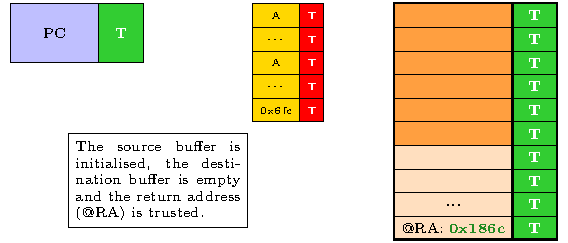
\includegraphics[width=\textwidth, page=1]{c3_vulnerabilities_assessment/img/buffer_overflow/schemaPedagogique.pdf}
        \caption{Initialisation}
        \label{fig:rop_attack_1}
    \end{subfigure}
    \hfill
    \begin{subfigure}[b]{0.49\textwidth}
        \includegraphics[width=\textwidth, page=2]{c3_vulnerabilities_assessment/img/buffer_overflow/schemaPedagogique.pdf}
        \caption{Copy of the source buffer into the destination buffer}
        \label{fig:rop_attack_2}
    \end{subfigure}
    \hfill
    \begin{subfigure}[b]{0.49\textwidth}
        \includegraphics[width=\textwidth, page=3]{c3_vulnerabilities_assessment/img/buffer_overflow/schemaPedagogique.pdf}
        \caption{An overflow occurs, the $ra$ register is overwritten}
        \label{fig:rop_attack_3}
    \end{subfigure}
    \hfill
    \begin{subfigure}[b]{0.49\textwidth}
        \includegraphics[width=\textwidth, page=4]{c3_vulnerabilities_assessment/img/buffer_overflow/schemaPedagogique.pdf}
        \caption{Corrupted $ra$ register is loaded into the PC}
        \label{fig:rop_attack_4}
    \end{subfigure}
    \hfill
    \begin{subfigure}[b]{0.49\textwidth}
        \includegraphics[width=\textwidth, page=5]{c3_vulnerabilities_assessment/img/buffer_overflow/schemaPedagogique.pdf}
        \caption{PC address instruction is fetched}
        \label{fig:rop_attack_5}
    \end{subfigure}
    \caption{Representation of how the ROP attack works}
    \label{fig:rop_attack}
\end{figure}

%%%%%%%%%%%%%%%%%%%%%%%%%%%%%%%%%%%%%%%%%%
\subsection{Second use case: Format String (WU-FTPd)}
The second use case is a format string attack\footnote{\url{https://github.com/sld-columbia/riscv-dift/tree/master/pulpino_apps_dift/wu-ftpd}} overwriting the return address of a function to jump to a shellcode and starts its execution.  This use case uses the first security policy from Table~\ref{tab:tpr} and Table~\ref{tab:tcr}.
This attack exploits the \verb|printf()| function from the C library. It uses the \verb|%u| and \verb|%n| formats (see Chapter 12, Section 12.14.3 in~\cite{gnu_lib_c} for detailed information) to write the targeted address.

Listing~\ref{code:wu_ftpd} shows the C code of this use case. The \texttt{echo} function assign the \textit{x8} register to a variable '\verb|i|' which goes into another variable '\verb|a|'.
The lines 13-14 are used to initialise the tag associated to the variable '\verb|a|'. This variable `\verb|a|' is user-defined, so it is tagged as untrusted for DIFT computation.
The vulnerable statement is the \verb|printf| statement in line 16.
The format \verb|%u| is used to print unsigned integer characters.
The format \verb|%n| is used to store in memory the number of characters printed by the \verb|printf()| function, the argument it takes is a pointer to a signed int value. 

The execution of the \verb|printf| at line 16 leads to write in memory 224 (0xe0) at address (a-4), 224+35 so 259 (0x103) at address (a-3), and 512 (0x200) at addresses (a-2) and (a-1). The attacker's objective is to overwrite the return address with `\textit{0x3e0}' which represent the address of the first function, called \textit{secretFunction} in Listing~\ref{code:wu_ftpd}. In this case, security policy prohibits the use of untrusted variables as store addresses. Since variable `\verb|a|' is untrusted, the DIFT protection raises an exception when storing a value at memory address \verb|(a-4)|. This use case has been chosen to activate the load/store modes of the DIFT policy. 

\begin{lstlisting}[style=topPosition, language=C,label=code:wu_ftpd, caption=WU-FTPd C code]
void secretFunction(){
    printf("Congratulations!\n");
    printf("You have entered in the secret function!\n");

    exit(0);
}

void echo(){
    int a;
    register int i asm("x8");
    a = i;

    asm volatile ("p.spsw x0, 0(%[a]);"                
                ::[a] "r" (&a));

    printf("%224u%n%35u%n%253u%n%n", 1, (int*) (a-4), 1, (int*) (a-3), 1, (int*) (a-2), (int*) (a-1));

    return;
}

int main(int argc, char* argv[]){ 
    volatile int a = 1;

    if(a)
        echo();
    else
        secretFunction();

    return 0;
}\end{lstlisting}

Table~\ref{table:ftpdOverwriteMemory} represents the different steps to overwrite the memory with the exact address of the malicious function. We can see that after each write and the right shift of the writing, the address appears. Finally, we have the address '\textit{000002000003E0}' in memory from 'A+2' to 'A-4' but as an address is on 32-bits in our architecture, the address fetched by the pipeline is only '\textit{000003E0}'.

\begin{table}[t]
    \centering
    \caption{Memory overwrite}
    \label{table:ftpdOverwriteMemory}
    \begin{tabular}{l|ccccccc}
        \toprule
        Address & A-4 & A-3 & A-2 & A-1 & A & A+1 & A+2 \\ \midrule
        A-4     & \textit{0xE0} & \textit{0x00} & \textit{0x00} & \textit{0x00} & \textit{}     & \textit{}     & \textit{}     \\
        A-3     & \textit{}     & \textit{0x03} & \textit{0x01} & \textit{0x00} & \textit{0x00} & \textit{}     & \textit{}     \\
        A-2     & \textit{}     & \textit{}     & \textit{0x00} & \textit{0x02} & \textit{0x00} & \textit{0x00} & \textit{}     \\
        A-1     & \textit{}     & \textit{}     & \textit{}     & \textit{0x00} & \textit{0x02} & \textit{0x00} & \textit{0x00} \\ \midrule
        Memory & {0xE0}    & {0x03}    & 0x00          & 0x00          & 0x02          & 0x00          & 0x00          \\
        \bottomrule
    \end{tabular}
\end{table}


%%%%%%%%%%%%%%%%%%%%%%%%%%%%%%%%%%%%%%%%%%%%%%%%%%%%%%%%%%%%%%%%%%%%%%%%%%%%%%%%%%%%%%%%%%%%%%%
\section{Vulnerability assessment}
\label{section:vuln_assessment}
In order to analyse the behaviour of the processor at application runtime against Fault Injection Attacks, we have simulated some fault injections campaigns in which we inject fault inside the 55 registers associated to the DIFT, which correspond to 127 bits in total. Table~\ref{tab:registersDIFT} shows the repartition of these registers in every pipeline stage of the RI5CY core and the number of associated bits. This work has been published in ACM Sensors S\&P~\cite{PLG-22-SensorsSP}.% and the same analysis is available in it.

\begin{table}[t]
    \centering
    \caption{Numbers of registers and quantity of bits represented}
    \label{tab:registersDIFT}
    \begin{tabular}{@{}ccc@{}}
        \toprule
        \textbf{HDL Module} & \textbf{Number of registers} & \textbf{Number of bits in registers} \\ \midrule
        Instruction Fetch Stage & 2 & 2 \\
        Instruction Decode Stage & 14 & 19 \\
        Register File Tag & 1 & 32 \\
        Execution Stage & 1 & 1 \\
        Control and Status Registers & 2 & 64 \\
        Load/Store Unit & 4 & 9 \\
        \midrule
        \midrule
        \textbf{Total} & \textbf{\textbf{24}} & \textbf{\textbf{127}} \\
        \bottomrule
    \end{tabular}
\end{table}

We assess the design with fault injection campaigns. With their results associated, we can deduce which registers are vulnerable with the cycle associated and the fault model. This assessment is done for each use case for a more precise analysis and to understand how the tag is propagated and checked before the exception.

%%%%%%%%%%%%%%%%%%%%%%%%%%%%%%%%%%%%%%%%%%
\subsection{Fault model for vulnerability assessment}
In this vulnerability assessment, we consider an attacker able to inject faults into DIFT-related registers leading to \textit{set to 0}, \textit{set to 1}, and \textit{single bit-flip in one register at a given clock cycle}. To bypass the DIFT mechanism, the main attacker's goal is to prevent an exception being raised. To reach this objective, any DIFT-related register maintaining tag value, driving the tag propagation or the tag update process or maintaining the security policy configuration can be targeted.


%%%%%%%%%%%%%%%%%%%%%%%%%%%%%%%%%%%%%%%%%%
\subsection{First use case: Buffer overflow}
Table~\ref{tab:end_sim_from_time_fault_register_bo} shows that 22 fault injections in four different DIFT-related registers can lead to a successful attack despite the DIFT mechanism (i.e., DIFT protection is bypassed). 
For example, it shows that a fault injection targeting the~\textit{pc\_if\_o\_tag} register can defeat the DIFT protection if a fault is injected at cycle 3431 using a bit-flip or a set to 0 fault type.
Furthermore, Table~\ref{tab:end_sim_from_time_fault_register_bo} shows that five different cycles can be targeted for the attack to succeed. In most cases, \textit{bit-flip} leads to a successful injection with 11 successes over 22. Faults in \textit{tpr\_q} and \textit{tcr\_q} are successful, since these registers maintain the propagation rules and the security policy configuration (see Table~\ref{tab:tpr} and Table~\ref{tab:tcr} for more details about each bit position). Both \textit{pc\_if\_o\_tag} and \textit{rf\_reg[1]} are also critical registers for this use case. Indeed, \textit{pc\_if\_o\_tag} allows the propagation of the PC tag while \textit{rf\_reg[1]} stores the tag of the return address register $ra$.

\begin{table}[t]
    \small
    \centering
    \setlength{\tabcolsep}{4pt}
    \caption{Buffer overflow: success per register, fault type and simulation time}
    \label{tab:end_sim_from_time_fault_register_bo}
    \begin{tabular}{@{}lccccccccccccccc@{}}
        \toprule
         & \multicolumn{3}{c}{Cycle 3428} & \multicolumn{3}{c}{Cycle 3429} & \multicolumn{3}{c}{Cycle 3430} & \multicolumn{3}{c}{Cycle 3431} & \multicolumn{3}{c}{Cycle 3432} \\\cmidrule(lr){2-4}\cmidrule(lr){5-7}\cmidrule(lr){8-10}\cmidrule(lr){11-13}\cmidrule(lr){14-16}
         & set0 & set1 & bit-flip & set0 & set1 & bit-flip & set0 & set1 & bit-flip & set0 & set1 & bit-flip & set0 & set1 & bit-flip \\
        \midrule
        pc\_if\_o\_tag &  &  &  &  &  &  &  &  &  & \checkmark &  & \checkmark &  &  &  \\
        rf\_reg[1] &  &  &  &  &  &  & \checkmark &  & \checkmark &  &  &  &  &  &  \\
        tcr\_q & \checkmark &  &  & \checkmark &  &  & \checkmark &  &  & \checkmark &  &  & \checkmark &  &  \\
        \rowcolor{LightGray} tcr\_q[21] &&& \checkmark &&& \checkmark &&& \checkmark &&& \checkmark &&& \checkmark \\
        tpr\_q & \checkmark & \checkmark &  & \checkmark & \checkmark &  &  &  &  &  &  &  &  &  &  \\
        \rowcolor{LightGray} tpr\_q[12] &&& \checkmark &&& \checkmark &  &  &&&&&&&  \\
        \rowcolor{LightGray} tpr\_q[15] &&& \checkmark &&& \checkmark &  &  &&&&&&&  \\
        \bottomrule
    \end{tabular}
\end{table}

Now that we have these results, we can analyse them and present an in-depth analysis of the simulation results leading to successful attacks. The aim is to understand why an attack succeeds. For that purpose, we study the propagation of the fault through both temporal and logical views. Most of the faults targeting both TPR and TCR registers are not detailed in this section. Indeed, these faults mainly target the DIFT configuration and not the tag propagation and tag-checking computations. Faults targeting these registers can be performed in any cycle prior to their use. 

Figure~\ref{fig:study_buffer_overflow_tag_propagation} presents the $ra$ register tag propagation in the context of the first use case for a non-faulty execution. It focuses on three clock cycles from the decoding of a \verb|jalr| instruction (i.e.,  returning from the called function) to the DIFT exception due to a security policy violation. 
In cycle 3430, this tag is extracted from the \textit{register file tag} (i.e., from \textit{rf\_reg[1]}). In cycle 3431, it is propagated to the \textit{pc\_if\_o\_tag} register. Then, in cycle 3432, it is propagated in the \textit{pc\_id\_o\_tag} register and the first shellcode instruction is decoded. Since $ra$ is tagged as untrusted and the security policy prohibits the use of tagged data in PC (\textit{Execute Check} bit = 1 in Table~\ref{tab:tcr}), an exception is raised during the tag check process, which is performed in parallel of the first shellcode instruction decoding.

Figure~\ref{fig:study_buffer_overflow_tag_propagation} illustrates the reason behind the sensitivity of registers \textit{rf\_reg[1]} and \textit{pc\_if\_o\_tag} at cycles 3430, 3431 and 3432 highlighted in  Table~\ref{tab:end_sim_from_time_fault_register_bo}. We can note that \textit{pc\_id\_o\_tag} register does not appear in Table~\ref{tab:end_sim_from_time_fault_register_bo} while Figure~\ref{fig:study_buffer_overflow_tag_propagation} shows its role during tag propagation. Actually, this register gets its value from \textit{pc\_if\_o\_tag}, so a fault injection in this register only delays the exception. 

\begin{figure}[ht]
    \centering
    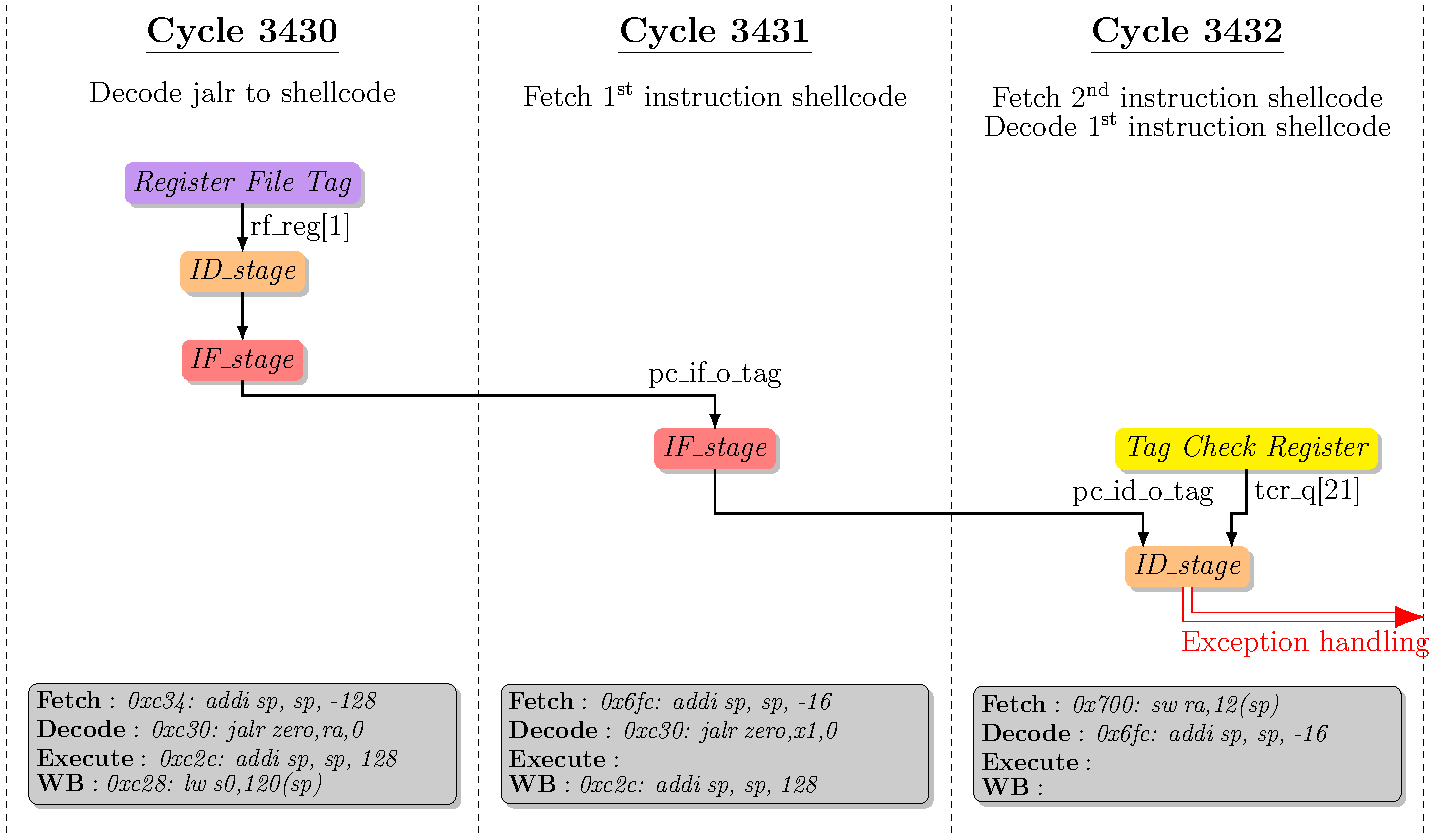
\includegraphics[width=\textwidth]{c3_vulnerabilities_assessment/img/buffer_overflow/bufferOverflowAttack_short.pdf}
    \caption{Tag propagation in a buffer overflow attack}
    \label{fig:study_buffer_overflow_tag_propagation}
\end{figure}

To further study the propagation of the fault, Figure~\ref{fig:buffer_overflow_tag_propagation} illustrates the logical relations between the DIFT-related registers (yellow boxes) and control signals or processor registers (grey boxes) driving the illegal instruction exception signal (red box). This figure does not describe the actual hardware architecture but highlights the logic path leading to an exception raise. An attacker performing fault injections would like to drive the exception signal to `0' to defeat the D-RI5CY DIFT solution. Figure~\ref{fig:buffer_overflow_tag_propagation} shows that a single fault could lead to a successful injection since all logic paths are built with \textit{AND} gates. For instance, if register \textit{rf\_reg[1]} is set to 0, the tag will be propagated from \textit{gate 1} to \textit{gate 4}. Then, \textit{gate 5} inputs are \textit{tcr\_q[21]} (i.e., `1') and \textit{pc\_id\_o\_tag} (i.e., `0',  \textit{gate 4} output). Thus, \textit{gate 5} output is driven to `0', disabling the exception. 
From Figure~\ref{fig:buffer_overflow_tag_propagation}, three fault propagation paths can be identified: from \textit{gate 1} to \textit{gate 5} if the fault is injected into \textit{rf\_reg[1]}, from \textit{gate 4} to \textit{gate 5} if a fault is injected into \textit{pc\_if\_o\_tag} and through \textit{gate 5} if a fault is injected into either the \textit{tcr\_q} or \textit{pc\_id\_o\_tag}.
Analysis of Figure~\ref{fig:buffer_overflow_tag_propagation} strengthens the results presented in Table~\ref{tab:end_sim_from_time_fault_register_bo} where \textit{set to 0} and \textit{bit-flip} fault types lead to successful attacks. The root cause is that the propagation paths consist entirely of \textit{AND} gates. 

\begin{figure}[ht]
    \centering
    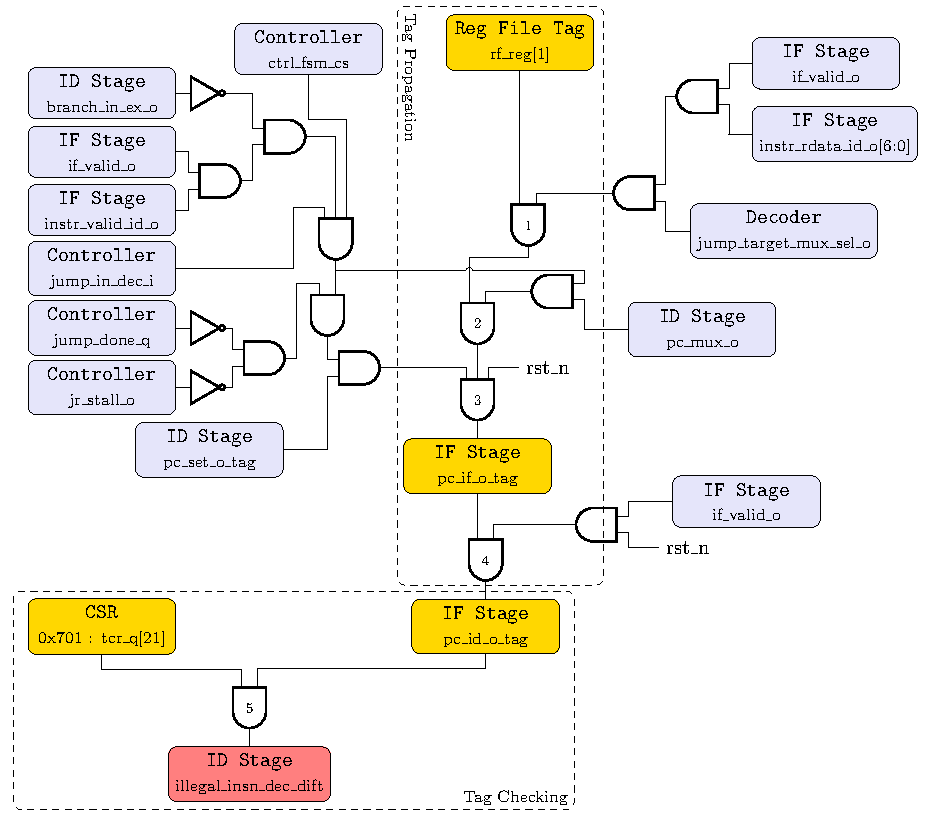
\includegraphics[width=\textwidth]{c3_vulnerabilities_assessment/img/buffer_overflow/arborescence_bufferOverflow.pdf}
    \caption{Logic description of the exception driving in a buffer overflow attack}
    \label{fig:buffer_overflow_tag_propagation}
\end{figure}

%%%%%%%%%%%%%%%%%%%%%%%%%%%%%%%%%%%%%%%%%%
\subsection{Second use case: Format string (WU-FTPd)}
Table~\ref{tab:end_sim_from_time_fault_register_mo} shows that 52 fault injections in 10 DIFT-related registers can lead to a successful attack. 
Furthermore, it shows that 8 different cycles can be targeted for the attack to succeed. 29 successes over 52 are obtained with the \textit{bit-flip} fault type. 
\textit{alu\_operand\_a\_ex\_o\_tag}, \textit{alu\_operand\_b\_ex\_o\_tag} and \textit{alu\_operator\_o\_mode} registers are critical during cycles 52477 and 52478 since they are used for tag propagation related to the C statement \verb|(a-4)|. \textit{alu\_operand\_a\_ex\_o\_tag} and \textit{alu\_operand\_b\_ex\_o\_tag} sequentially store the tag associated to `\verb|a|' while \textit{alu\_operator\_o\_mode} stores the propagation rule according to the TPR configuration (see Table~\ref{tab:tpr}). \textit{regfile\_alu\_waddr\_ex\_o\_tag} stores the destination register index in which the tag resulting from tag propagation should be written.
\textit{check\_s1\_o\_tag} maintains the TCR value from the decode stage to the execution stage, it is compared to the value of the operand tag for tag checking.
\textit{rf\_reg[15]} stores the tag associated with the `\verb|a|' variable.
\textit{store\_dest\_addr\_ex\_o\_tag} maintains the tag of the destination address during a store instruction in the execute stage. 
\textit{use\_store\_ops\_ex\_o} drives a multiplexer to propagate the value stored in \textit{store\_dest\_addr\_ex\_o\_tag} register to the tag checking module.
Finally, faults in \textit{tpr\_q} and \textit{tcr\_q} are successful, since these registers maintain the propagation rules and the security policy configuration. 
The last two registers, \textit{tpr\_q} and \textit{tcr\_q} are critical when we fault the bit 12 of TPR because the load/store mode which is set to \textit{10} but if we change it the propagation policy will change and then the tag will not be propagated as a mode set to \textit{11} will clear the tag. A bit-flip at bit 15 will impact the behaviour as it stores the load/store enable source tag. Finally, bit 20 of TCR store the load/store check destination address tag, which is used when the program wants to store at the address (a-4).

Figure~\ref{fig:study_mem_overwriting_tag_propagation} details the tag propagation in the context of a format string attack case for a non-faulty execution and illustrates the reason behind the sensitivity of registers highlighted in Table~\ref{tab:end_sim_from_time_fault_register_mo}.
Figure~\ref{fig:study_mem_overwriting_tag_propagation} focuses on three clock cycles dedicated to the instruction \verb|sw a4,0(a5)| decoding and execution which should lead to the storage of the value 224 at address (a-4). 
In cycles 52482 and 52483, \verb|sw a4,0(a5)| is decoded and the source operands tag are retrieved from the tag register file. Particularly, the store destination address is retrieved from \textit{rf\_reg[15]} and stored in register \textit{store\_dest\_addr\_ex\_o\_tag}. In cycle 52484, the destination address of the store operation is computed by the processor Arithmetic Logic Unit (ALU).
In parallel, \textit{alu\_operator\_o\_mode}, \textit{alu\_operand\_a\_ex\_o\_tag}, \textit{alu\_operand\_b\_ex\_o\_tag}, \textit{store\_dest\_addr\_ex\_o\_tag} and \textit{check\_s1\_o\_tag} registers drives the tag computation corresponding to the destination address. 
\textit{use\_store\_ops\_ex\_o} drives a multiplexer to propagate the value stored in \textit{alu\_operand\_a\_ex\_o\_tag} register to the tag checking module. 
\textit{alu\_operand\_a\_ex\_o\_tag} and \textit{alu\_operand\_b\_ex\_o\_tag} sequentially store the tag associated to `\verb|a|' while \textit{alu\_operator\_o\_mode} stores the propagation rule according to the TPR configuration (see Table~\ref{tab:tpr}).
\textit{check\_s1\_o\_tag} maintains the TCR value from the decode stage to the execution stage, it is compared to the value of the operand tag for tag checking.
Then, the store should be executed in the Execute stage. However, the tag associated with the store destination address is set to 1 due to tag propagation (since it is computed from variable `\verb|a|'). 
Since the security policy prohibits the use of data tagged as \textit{untrusted} as a store instruction destination address (\textit{Load/Store Check} field of TCR = 1010), an exception is raised.
\textit{use\_store\_ops\_ex\_o}, highlighted in Table~\ref{tab:end_sim_from_time_fault_register_mo} but not shown in Figure~\ref{fig:study_mem_overwriting_tag_propagation}, drives a multiplexer leading to the propagation of register \textit{store\_dest\_addr\_ex\_o\_tag}.

\begin{landscape}
    \begin{table}[t]
        \footnotesize
        \centering
        \caption{Format string attack: success per register, fault type and simulation time}
        \label{tab:end_sim_from_time_fault_register_mo}
        \setlength{\tabcolsep}{1pt}
        \begin{tabular}{@{}lcccccccccccccccccccccccc@{}}
            \toprule
            & \multicolumn{3}{c}{Cycle 52477} & \multicolumn{3}{c}{Cycle 52478} & \multicolumn{3}{c}{Cycle 52479} & \multicolumn{3}{c}{Cycle 52480} & \multicolumn{3}{c}{Cycle 52481} & \multicolumn{3}{c}{Cycle 52482} & \multicolumn{3}{c}{Cycle 52483} & \multicolumn{3}{c}{Cycle 52484} \\\cmidrule(lr){2-4}\cmidrule(lr){5-7}\cmidrule(lr){8-10}\cmidrule(lr){11-13}\cmidrule(lr){14-16}\cmidrule(lr){17-19}\cmidrule(lr){20-22}\cmidrule(lr){23-25}
            & set0 & set1 & bit-flip & set0 & set1 & bit-flip & set0 & set1 & bit-flip & set0 & set1 & bit-flip & set0 & set1 & bit-flip & set0 & set1 & bit-flip & set0 & set1 & bit-flip & set0 & set1 & bit-flip \\
            \midrule
            alu\_operand\_a\_ex\_o\_tag & \checkmark &  & \checkmark &  &  &  &  &  &  &  &  &  &  &  &  &  &  &  &  &  &  \\
            alu\_operand\_b\_ex\_o\_tag &&&& \checkmark &  & \checkmark &  &  &  &  &  &  &  &  &  &  &  &  &  &  &  &  &  &  \\
            alu\_operator\_o\_mode &\checkmark & \checkmark && \checkmark & \checkmark &  &  &  &  &  &  &  &  &  &  &  &  &  &  &  &  &  &  &  \\
            \rowcolor{LightGray} alu\_operator\_o\_mode[0] &&& \checkmark &&& \checkmark &  &  &  &  &  &&&&&&&&&&&&&  \\
            \rowcolor{LightGray} alu\_operator\_o\_mode[1] &&& \checkmark &&& \checkmark &  &  &  &  &  &&&&&&&&&&&&&  \\
            check\_s1\_o\_tag &&&&  &  &  &  &  &  &  &  &  &  &  &  &  &  &  &  &  &  & \checkmark &  & \checkmark \\
            regfile\_alu\_waddr\_ex\_o\_tag[1] &&&&  &  &  &  &  &  &  &  &  &  &  & \checkmark &  &  &  &  &  &  &  &  &  \\
            rf\_reg[15] &&&&  &  &  &  &  &  &  &  &  &  &  &  & \checkmark &  & \checkmark & \checkmark &  & \checkmark &  &  &  \\
            store\_dest\_addr\_ex\_o\_tag &&&&  &  &  &  &  &  &  &  &  &  &  &  &  &  &  &  &  &  & \checkmark &  & \checkmark \\
            tcr\_q & \checkmark &&& \checkmark &  &  & \checkmark &  &  & \checkmark &  &  & \checkmark &  &  & \checkmark &  &  & \checkmark &  &  &  &  &  \\
            \rowcolor{LightGray} tcr\_q[20] &&& \checkmark &&& \checkmark &&& \checkmark &&& \checkmark &&& \checkmark &&& \checkmark &&& \checkmark &&&  \\
            tpr\_q && \checkmark &&  & \checkmark &  &  & \checkmark &  &  & \checkmark &  &  & \checkmark &  &  &  &  &  &  &  &  &  &  \\
            \rowcolor{LightGray} tpr\_q[12] &&& \checkmark &&& \checkmark &&& \checkmark &&& \checkmark &&& \checkmark &  &  &&&&&&&  \\
            \rowcolor{LightGray} tpr\_q[15] &&& \checkmark &&& \checkmark &&& \checkmark &&& \checkmark &&& \checkmark &  &  &&&&&&&  \\
            use\_store\_ops\_ex\_o &&&&  &  &  &  &  &  &  &  &  &  &  &  &  &  &  &  &  &  & \checkmark &  & \checkmark \\
            \bottomrule
        \end{tabular}
    \end{table}
\end{landscape}

 \begin{figure}[ht]
    \centering
    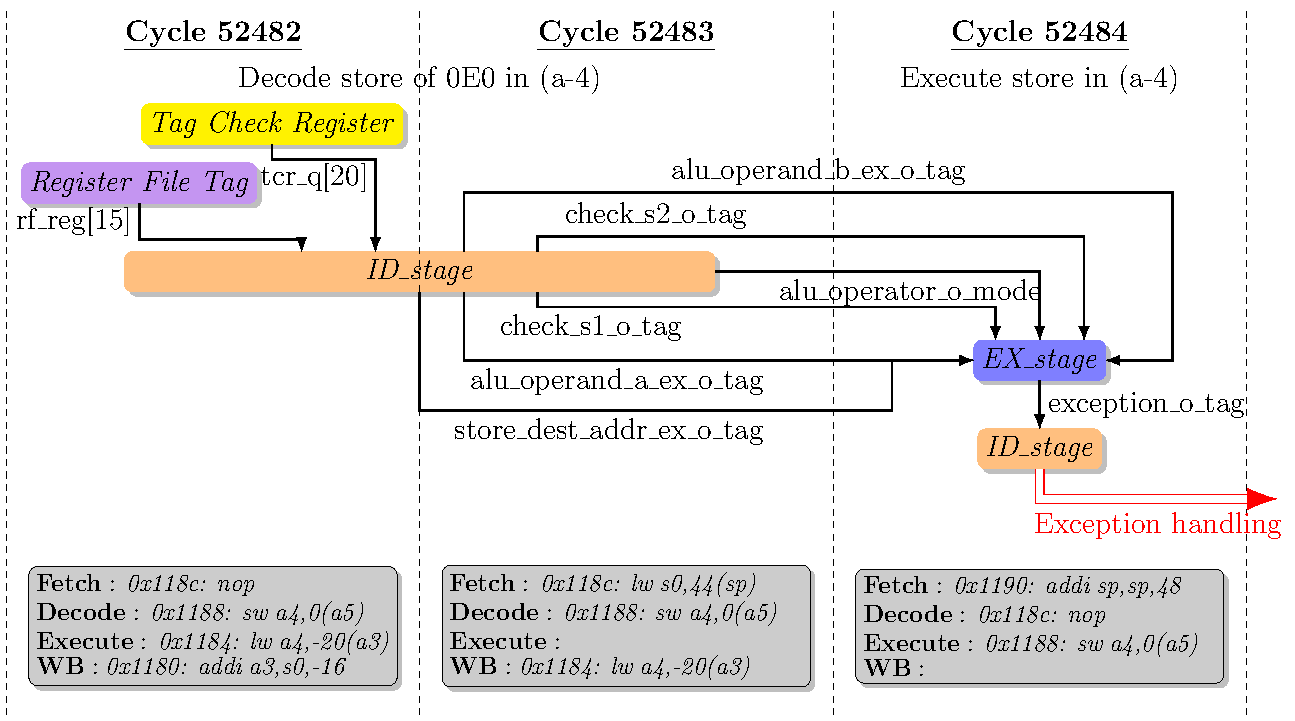
\includegraphics[width=\linewidth]{c3_vulnerabilities_assessment/img/wuftpd/full_ftpd_short.pdf}
    \caption{Tag propagation in a format string attack}
    \label{fig:study_mem_overwriting_tag_propagation}
 \end{figure}

To further study the propagation of the fault, Figure~\ref{fig:mem_overwriting_tag_propagation} illustrates the logical relations between the DIFT-related registers (yellow boxes) and control signals or processor registers (gray boxes) driving the illegal instruction exception signal (red box) for the second use case. 
Figure~\ref{fig:mem_overwriting_tag_propagation} shows that a single fault could lead to a successful injection, since all logic paths are built with \textit{AND} gates. For instance, if register \textit{rf\_reg[15]} is set to 0, this tag value will be propagated from \textit{gate 8} to \textit{gate 11} and to \textit{mux 12}. Then, since \textit{mux 12} output drives one \textit{gate 3} input, \textit{gate 3} output is driven to `0', the exception is disabled. 
From Figure~\ref{fig:mem_overwriting_tag_propagation}, seven fault propagation paths can be identified: 
from \textit{gate 1} to \textit{gate 3} if the fault is injected into \textit{tcr\_q[20]},
through \textit{gate 3} if a fault is injected into \textit{check\_s1\_o\_tag},
from \textit{gate 4} or \textit{gate 5} to \textit{gate 3} if a fault is injected into \textit{alu\_operand\_b\_ex\_o\_tag} or \textit{alu\_operand\_a\_ex\_o\_tag},
from \textit{mux 6} to \textit{gate 3} if a fault is injected into \textit{alu\_operator\_o\_mode},
from \textit{mux 7} to \textit{gate 3} if a fault is injected into \textit{regfile\_alu\_waddr\_ex\_o\_tag},
from \textit{gate 8} to \textit{gate 3} if a fault is injected in the tag register file (i.e., register \textit{rf\_reg[15]}) and
from \textit{mux 11} to \textit{gate 3} if a fault is injected in either \textit{store\_dest\_addr\_ex\_o\_tag} or \textit{use\_store\_ops\_ex\_o}.
Analysis of Figure~\ref{fig:mem_overwriting_tag_propagation} reinforces the results presented in Table~\ref{tab:end_sim_from_time_fault_register_mo} where \textit{set to 0} and \textit{bit-flip} fault types lead to successful attacks. As with the first use case, the main cause is that the propagation paths are fully made of \textit{AND} gates. As shown in Table~\ref{tab:end_sim_from_time_fault_register_mo} \textit{alu\_operator\_o\_mode} register is sensitive to \textit{set to 0} and \textit{set to 1} fault types. Indeed, this register determines the tag propagation according to TPR. The tag propagation is disabled when a TPR field is set to `00' and the output tag is set to 0 (i.e., trusted) when a TPR field is set to `11'. 

 \begin{figure}[ht]
    \centering
    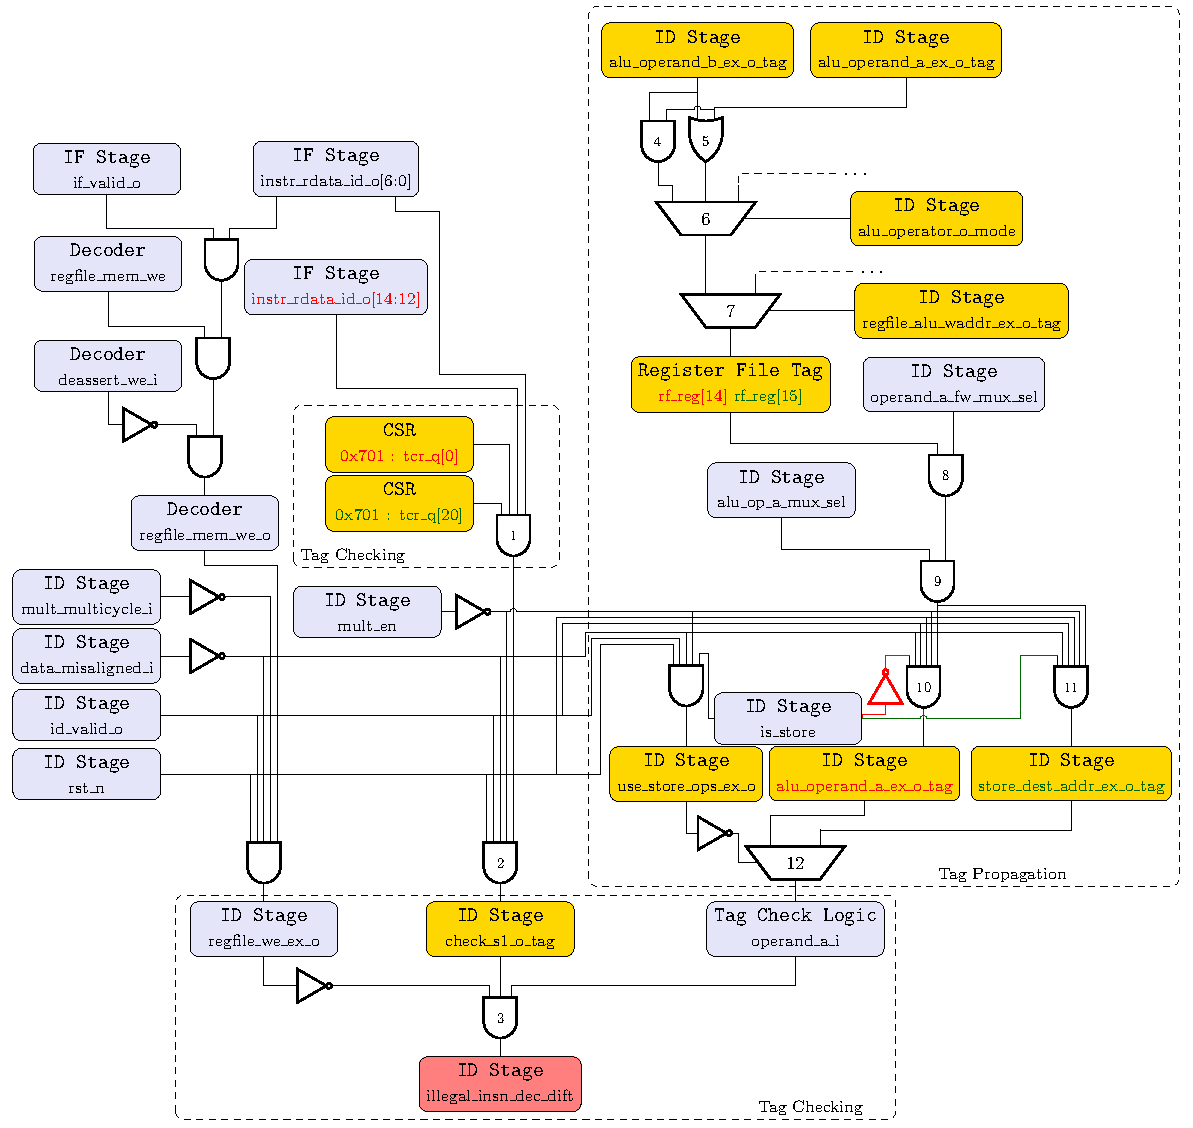
\includegraphics[width=\linewidth]{c3_vulnerabilities_assessment/img/wuftpd/arborescence_v3_wuftpd.pdf}
    \caption{Logic description of the exception driving in a format string attack}
    \label{fig:mem_overwriting_tag_propagation}
 \end{figure}


%%%%%%%%%%%%%%%%%%%%%%%%%%%%%%%%%%%%%%%%%%
\subsection{Third use case: Compare/Compute}
Table~\ref{tab:end_sim_from_time_fault_register_secpoV3} shows that 19 fault injections in 6 DIFT-related registers can lead to a successful attack. Furthermore, it shows that 4 different cycles can be targeted for the attack to succeed. The highest success rate is obtained with the \textit{bit-flip} fault type, with 10 successes over 19. 
Faults in \textit{rf\_reg[14]} and \textit{alu\_operand\_a\_ex\_o\_tag} are successful, since these registers store the tag associated to variable \verb|a| during tag propagation. \textit{check\_s1\_o\_tag} maintains one configuration bit from \textit{tcr\_q} during tag checking.
\textit{use\_store\_ops\_ex\_o} drives a multiplexer to propagate the value stored in \textit{alu\_operand\_a\_ex\_o\_tag} register to the tag checking module. 
For this case, the critical registers can be found in previous case, \textit{alu\_operand\_a\_ex\_o\_tag} propagate the tag of the tagged variable in the code (variable \verb|a|). 
Finally, observations for both \textit{tpr\_q} and \textit{tcr\_q} are similar than for previous case studies. 
Finally, faults in \textit{tpr\_q} and \textit{tcr\_q} are successful, since these registers maintain the propagation rules and the security policy configuration. 

\begin{table}[t]
   \small
   \centering
   \caption{Compare/compute: number of faults per register, per fault type and per cycle}
   \label{tab:end_sim_from_time_fault_register_secpoV3}
   \setlength{\tabcolsep}{4pt}
   \begin{tabular}{@{}lcccccccccccc@{}}
        \toprule
        & \multicolumn{3}{c}{Cycle 832} & \multicolumn{3}{c}{Cycle 833} & \multicolumn{3}{c}{Cycle 834} & \multicolumn{3}{c}{Cycle 835} \\\cmidrule(lr){2-4}\cmidrule(lr){5-7}\cmidrule(lr){8-10}\cmidrule(lr){11-13}
        & set0 & set1 & bit-flip & set0 & set1 & bit-flip & set0 & set1 & bit-flip & set0 & set1 & bit-flip \\
        \midrule
        alu\_operand\_a\_ex\_o\_tag &  &  &  &  &  &  &  &  &  & \checkmark &  & \checkmark \\
        check\_s1\_o\_tag &  &  &  &  &  &  &  &  &  & \checkmark &  & \checkmark \\
        rf\_reg[14] &  &  &  & \checkmark &  & \checkmark & \checkmark &  & \checkmark &  &  &  \\
        tcr\_q & \checkmark &  &  & \checkmark &  &  & \checkmark &  &  &  &  &  \\
        \rowcolor{LightGray} tcr\_q[0] &&& \checkmark &&& \checkmark &&& \checkmark &&&  \\
        tpr\_q &  & \checkmark &  &  &  &  &  &  &  &  &  &  \\
        \rowcolor{LightGray} tpr\_q[12] &&& \checkmark &  &  &&&&&&&  \\
        \rowcolor{LightGray} tpr\_q[15] &&& \checkmark &  &  &&&&&&&  \\
        use\_store\_ops\_ex\_o &  &  &  &  &  &  &  &  &  &  & \checkmark & \checkmark \\
        \bottomrule
    \end{tabular}
\end{table}

Figure~\ref{fig:study_attack_propag_v3_tag_propagation} focuses on the three cycles, represented in red, corresponding to \verb|add a5,a4,a5| instruction (C statement \verb|(a+b)|) decoding and execution in the context of the third use case. 
The instruction \verb|add a5,a4,a5| is in decode stage during cycles 833 and 834 and the tag associated to the untrusted variable \verb|a| is retrieved from \textit{rf\_reg[14]}. In cycle 835, this addition is executed. In parallel, variable \verb|a| tag is propagated to the tag check logic unit, which behaviour is driven by \textit{check\_s1\_o\_tag} through \textit{alu\_operand\_a\_ex\_o\_tag}. Since the V2 security policy prohibits the use of untrusted data as a source operand of an arithmetic operation, an exception is raised. 

Figure~\ref{fig:study_attack_propag_v3_tag_propagation} illustrates the reason behind the sensitivity of registers \textit{rf\_reg[14]}, \textit{alu\_operand\_a\_ex\_o\_tag} and \textit{check\_s1\_o\_tag} highlighted in Table~\ref{tab:end_sim_from_time_fault_register_secpoV3}.
Note that \textit{use\_store\_ops\_ex\_o} does not appear in Figure~\ref{fig:study_attack_propag_v3_tag_propagation}. This register drives a multiplexer leading to tag propagation presented in Figure~\ref{fig:study_attack_propag_v3_tag_propagation}.

\begin{figure}[ht]
    \centering
    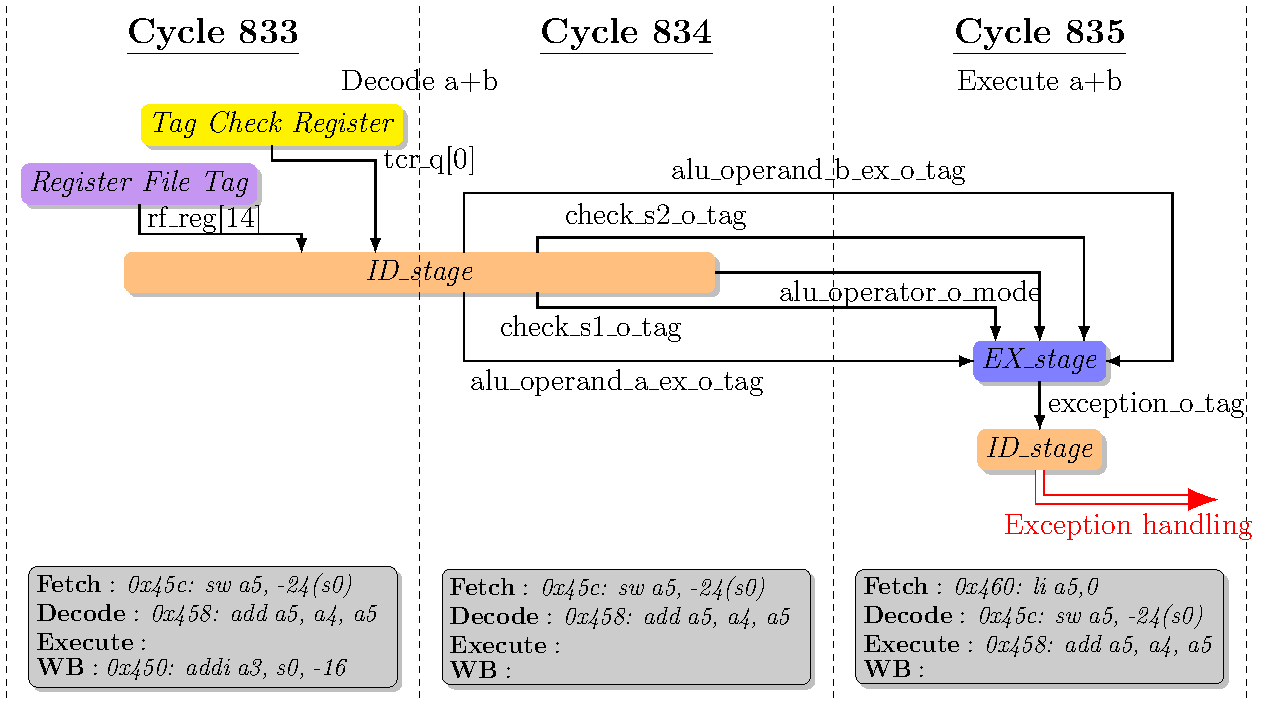
\includegraphics[width=\linewidth]{c3_vulnerabilities_assessment/img/comp_compu/attaquePropag_v3_short.pdf}
    \caption{Tag propagation in a computation case with the compare/compute use case}
    \label{fig:study_attack_propag_v3_tag_propagation}
\end{figure}

To further study the faults' propagation, Figure~\ref{fig:attack_propag_v3_tag_propagation} illustrates the logical relations between the DIFT-related registers (yellow boxes) and control signals or processor registers (gray boxes) driving the illegal instruction exception signal (red box).
Figure~\ref{fig:attack_propag_v3_tag_propagation} shows that a single fault could lead to a successful injection, since all logic paths are built with \textit{AND} gates. For instance, if register \textit{rf\_reg[14]} is set to 0, the tag will be propagated from \textit{gate 8} to \textit{gate 10} and to \textit{mux 12}. Then, since \textit{mux 12} output drives one \textit{gate 3} output, the exception is disabled.
From Figure~\ref{fig:attack_propag_v3_tag_propagation}, seven fault propagation paths can be identified. We won't go into detail here about the seven different paths, as they were mentioned in case 2, bearing in mind that colour differentiation must be taken into account (for example: \textit{alu\_operand\_a\_ex\_o\_tag} instead of \textit{store\_dest\_addr\_ex\_o\_tag}
from \textit{gate 1} to \textit{gate 3} if the fault is injected into \textit{tcr\_q[0]},
through \textit{gate 3} if a fault is injected into \textit{check\_s1\_o\_tag},
from \textit{gate 4} or \textit{gate 5} to \textit{gate 3} if a fault is injected into \textit{alu\_operand\_b\_ex\_o\_tag} or \textit{alu\_operand\_a\_ex\_o\_tag},
from \textit{mux 6} to \textit{gate 3} if a fault is injected into \textit{alu\_operator\_o\_mode},
from \textit{mux 7} to \textit{gate 3} if a fault is injected into \textit{regfile\_alu\_waddr\_ex\_o\_tag}, from \textit{gate 8} to \textit{gate 3} if a fault is injected into \textit{rf\_reg[14]}, and
from \textit{mux 11} to \textit{gate 3} if a fault is injected into either \textit{alu\_operand\_a\_ex\_o\_tag} or \textit{use\_store\_ops\_ex\_o}.
Analysis of Figure~\ref{fig:attack_propag_v3_tag_propagation} supports the results presented in Table~\ref{tab:end_sim_from_time_fault_register_secpoV3} where \textit{set to 0} and \textit{bit-flip} fault types lead to successful attacks. As with first and second use cases, the main reason is that the propagation paths are built entirely from \textit{AND} gates.

\begin{figure}[ht]
    \centering
    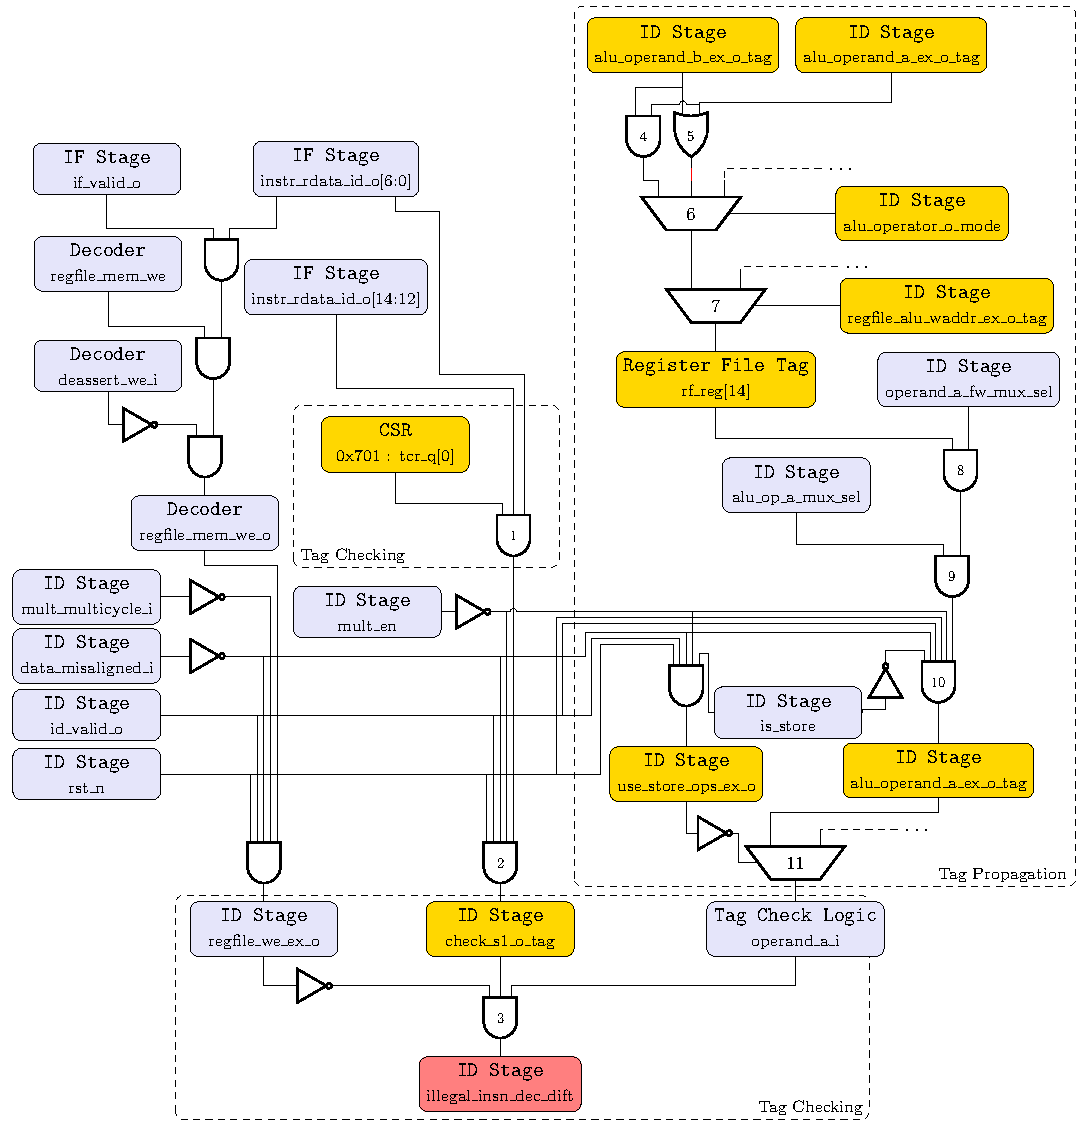
\includegraphics[width=\textwidth]{c3_vulnerabilities_assessment/img/comp_compu/arborescence_propagation.pdf}
    \caption{Logic representation of tag propagation in a computation case}
    \label{fig:attack_propag_v3_tag_propagation}
\end{figure}


%%%%%%%%%%%%%%%%%%%%%%%%%%%%%%%%%%%%%%%%%%%%%%%%%%%%%%%%%%%%%%%%%%%%%%%%%%%%%%%%%%%%%%%%%%%%%%%
\section{Summary}
In this section, we have described the processor, we will work on with its implementation of a hardware in-core DIFT. We have described how it works and how to use the DIFT part with the default configuration. Then, we described the different use cases we choose to work with to analyse the DIFT behaviour and assess its behaviour against fault injection attacks. Finally, we presented the vulnerability assessment on these use case using the D-RI5CY processor. We have shown that this DIFT implementation is vulnerable to FIA in different registers and depending on the application a different path is used and so different registers will be critical.
%%%%%%%%%%%%%%%%%%%%%%%%%%%%%%%%%%%%%%%%%%%%%%%%%%%%%%%%%%%%%%%%%%%%%%%%%%%%%%%%%%%%%%%%%%%%%%%

\clearemptydoublepage
\chapter{FISSA -- Fault Injection Simulation for Security Assessment}
\chaptermark{FISSA - Fault Injection Simulation for Security Assessment}
\label{chapter:fissa}
\minitoc

%%%%%%%%%%%%%%%%%%%%%%%%%%%%%%%%%%%%%%%%%%%%%%%%%%%%%%%%%%%%%%%%%%%%%%%%%%%%%%%%%%%%%%%%%%%%%%%
\section{Introduction}
This chapter introduces and presents a tool, called FISSA -- Fault Injection Simulation for Security Assessment --, created to automate fault injection attacks campaigns in simulation.
This work has been published in DSD 2024~\cite{PLG-24-dsd}.
The first section presents the state of the art of existing tools for FIA campaigns in simulation, formal methods, or even perform real world attacks.
The second section presents FISSA software architecture, details how FISSA works, and presents how to extend it.
The third section illustrates FISSA capacity through a use case from Section~\ref{section:uses_cases}.
Finally, the last section discusses and draws some perspectives for the tool's development and usability.

%%%%%%%%%%%%%%%%%%%%%%%%%%%%%%%%%%%%%%%%%%%%%%%%%%%%%%%%%%%%%%%%%%%%%%%%%%%%%%%%%%%%%%%%%%%%%%%
\section{Simulation tools for Fault Injection}

Addressing fault injection vulnerabilities is crucial. In general, fault attacks are conducted using physical equipment. Nonetheless, another approach exists that leverages simulators for fault testing. The main advantages of using simulators are they cost less money than physical setups, it is easier to make them work as they do not need specific skills, and they can be used during the conceptual stage.

This section presents recent works related to methods and tools for vulnerability assessment when considering fault injection attacks. For such vulnerability assessment, main strategies include actual fault injections, formal methods and simulations.
Another objective of fault injection in simulation is to address safety~\cite{FTMLLE-21-icsrs}. Safety concerns revolve around unintended, accidental faults, with a focus on system reliability and resilience. The aim is to verify the system’s capability to detect and recover from these faults, ensuring that no catastrophic consequences occur as a result of such failures. This process is crucial for validating the robustness of safety mechanisms in place.

\begin{table}[t]
    \centering
    \footnotesize
    \caption{Fault Injection based methods for vulnerability assessment comparison}
    \label{table:FI_type_comparison}
    \setlength{\tabcolsep}{1pt}
    \begin{tabular}{@{}lccccccc@{}}
        \toprule
                          & References  & Cost                                & \begin{tabular}[c]{@{}c@{}}Control over\\fault scenarios\end{tabular}       & Scalability                         & \begin{tabular}[c]{@{}c@{}}Speed of\\ execution\end{tabular}                                      & Realism                             & Expertise \\ \midrule
        Formal Methods    & \cite{BSSMG-21-tches, ANR-18-ices, BBCFGS-19-esorics, SVPMRDKMS-24-eprint}     & \textcolor{ForestGreen}{Very low}  & \textcolor{ForestGreen}{Very high}  & \textcolor{red}{Very low}           & \textcolor{red}{Low}                                    & \textcolor{red}{Low}                & \textcolor{red}{Very high} \\
        Simulations       & \cite{BLK-23-access, HGASO-21-fdtc, AB-23-acns, fisim, AWMN-20-host,TMZHM-23-iolts,WLRTF-22-tcad,GS-21-jcrypto,HSP-21-ifs}     & \textcolor{ForestGreen}{Very low}       & \textcolor{ForestGreen}{Very high}  & \textcolor{red}{Low}                & \textcolor{red}{Low}/\textcolor{ForestGreen}{Moderate}  & \textcolor{ForestGreen}{Moderate}   & \textcolor{ForestGreen}{Low} \\
        Actual FIA        & \cite{NNHRS-14-dsd,CMLCVR-11-crypto, BCNTW-06-procieee, BFP-19-tches, GBD-23-paine, CGVCBLC-22-cardis}     & \textcolor{Red}{Very high}           & \textcolor{Red}{Very low}           & \textcolor{ForestGreen}{Very high}  & \textcolor{ForestGreen}{Very high}                      & \textcolor{ForestGreen}{Very high}  & \textcolor{red}{Very high} \\
        \bottomrule
    \end{tabular}
\end{table}

Actual FIAs involve physically injecting faults into the target hardware using techniques such as variations in supply voltage or clock signal~\cite{BCNTW-06-procieee, BFP-19-tches}, laser pulses~\cite{BCNTW-06-procieee, CGVCBLC-22-cardis}, electromagnetic emanations~\cite{BCNTW-06-procieee} or X-Rays~\cite{GBD-23-paine}.
This approach offers valuable insights into the real impact of faults on hardware components.
However, a significant drawback of actual fault injections is that they demand considerable expertise to prepare the target, involving intricate setup procedures.
Additionally, this approach can only be executed once the physical circuit is available, potentially delaying the vulnerability assessment process until later stages of development.

Formal methods provide an advantage with mathematical proofs, ensuring a rigorous verification of the system's behaviour during fault injection experiments. Formal methods approaches such as~\cite{BSSMG-21-tches} allow the analysis of a circuit design in order to detect sensitive logic or sequential hardware elements. \cite{ANR-18-ices}, \cite{BBCFGS-19-esorics} and~\cite{SVPMRDKMS-24-eprint} present formal verification methods to analyse the behaviour of HDL implementation. However, this type of tool usually suffers from restrictions limiting its actual usage on a complete processor. Conventional formal approaches encounter scalability challenges due to limitations in verification techniques. In particular, the circuit structure it can analyse is usually limited (e.g. if there is a loop in the design).

Many simulators for fault injection attacks exist at different levels, to achieve different objectives, such as security at gate-level, cryptographic systems, study the impact of clock glitches, or even X-Ray. They can use Artificial Intelligence (AI) to enhance the detection. Another way to simulate fault injections is to use QEMU (Quick EMUlator)~\cite{BLK-23-access,HGASO-21-fdtc}.
QEMU is an open-source machine emulate the behaviour of a processor at a very fine-grain, using various optimizations to keep execution speed as close as possible to native system execution.
Bekele et al~\cite{BLK-23-access} present a survey of QEMU-based Fault Injection techniques. After discussing the various techniques proposed in the state of the art, they classify into categories and compare them.
Fault Injections simulations can be performed at processor instructions level. Authors of~\cite{AB-23-acns} explore the impact of fault injection attacks on software security. They evaluate four open-source fault simulators, comparing their techniques and suggest enhancing them with AI methods inspired by advances in cryptographic fault simulation. 
\cite{AWMN-20-host} introduces VerFI, a gate-level granularity fault simulator for hardware implementations. For instance, it has been used to spot an implementation mistake in ParTI~\cite{SMG-16-crypto}. However, this tool has been developed to check if implemented countermeasures can really protect against fault injection on cryptographic implementations, but it cannot evaluate components such as registers or memories.
\cite{fisim} is an open-source deterministic fault attack simulator prototype utilising the Unicorn Framework and Capstone disassembler.
Tebina et al.~\cite{TMZHM-23-iolts} introduce Ray-Spect, a tool to simulate fault injection using parametric degradation of MOSFETs transistors, which is typical of X-ray fault injection.
Wang et al.~\cite{WLRTF-22-tcad} developed a framework for fault injection assessment at gate-level with design specific security properties.
Grycel et al.~\cite{GS-21-jcrypto} present, SimpliFI, a simulation methodology to test fault attacks on embedded software using a hardware simulation of the processor running the software. It relies on post-layout netlist simulations to study the impact of fault injection techniques such as clock glitches.

In this work, we focus on RTL simulations, which provides a controlled virtual environment for injecting faults. There are several solutions of simulations in an HDL simulator like Questasim, Vivado, etc. \textit{Behavioural} simulation is used to detect functional issues and ensuring that the design behaves as expected. \textit{Post-synthesis} simulation verifies that the synthesised netlist matches the expected functionality. \textit{Timed} simulation is used to ensure that the design meets timing requirements and can operate at the specified clock frequency. And finally, \textit{post-implementation} simulations are used to verify that the implemented design meets all requirements and constraints, including those related to the physical layout on the target.
Post-synthesis, timed, and post-implementation simulations can be more difficult to apprehend. This is because HDL synthesis alters the names of the various hardware elements, making it more difficult to find the various elements targeted in the behavioural section.
Behavioural simulation-based fault injection offers the advantage of enabling designers to test their system at the early beginning of the design cycle, providing valuable insights and uncovering potential vulnerabilities early in the development process. However, a limitation lies in the potential lack of absolute fidelity to actual conditions, as simulations might not perfectly replicate all hardware intricacies, introducing a slight risk of overlooking certain faults that could manifest in the actual hardware.

Table~\ref{table:FI_type_comparison} shows a comparison between these four methods for vulnerability assessment when considering FIA regarding six metrics. These metrics are the financial cost of setting up the fault injection campaign, the control over fault scenarios (how configurable are the scenarios), scalability which refers to the method capacity to be applied to systems of different sizes or complexities, speed of execution of the campaign, realism of the fault injection campaign and the level of required expertise.
Table~\ref{table:FI_type_comparison} shows that no method is completely optimal. Each method has its own advantages and disadvantages and must be chosen by the designer according to the requirements and the available financial and human resources. Indeed, setting up an actual fault injection campaign requires much more expertise in this domain and also requires costly equipment, whereas setting up a simulation campaign can be easier for a circuit designer familiar with HDL simulation tools.
Table~\ref{table:FI_type_comparison} shows that simulation offers a good compromise to assess the security level of a circuit design. In particular, it provides an efficient solution for investigating security throughout the design cycle, enabling the concept of “Security by Design”.

%%%%%%%%%%%%%%%%%%%%%%%%%%%%%%%%%%%%%%%%%%%%%%%%%%%%%%%%%%%%%%%%%%%%%%%%%%%%%%%%%%%%%%%%%%%%%%%
\section{FISSA}
This section presents our open-source tool, FISSA, available on GitHub~\cite{fissa} under the CeCILL-B licence.

%%%%%%%%%%%%%%%%%%%%%%%%%%%%%%%%%%%%%%%%%%
\subsection{Main software architecture}
FISSA is designed to help circuit designers to analyse, at the early beginning of the development, the sensitivity to FIA of the developed circuit. FISSA relies on behavioural simulations.
Figure~\ref{fig:archi_fissa} presents the software architecture of FISSA.
It consists of three different modules: \textit{TCL generator}, \textit{Fault Injection Simulator} and \textit{Analyser}. The first and third modules correspond to a set of Python classes.

\textit{The TCL generator}, detailed in Section~\ref{subsec:tcl_gen}, relies on a configuration file and a target file to create a set of parameterised TCL scripts. These scripts are tailored based on the provided configuration file and are used to drive the fault injection simulation campaign.

\textit{Fault Injection Simulator}, detailed in Section~\ref{subsec:FIS}, performs the fault injection simulation campaign based on inputs files from \textit{TCL generator} for a circuit design described through HDL files and memory initialisation files. For that purpose it relies on an existing HDL simulator such as Questasim~\cite{questasim}, Verilator~\cite{verilator}, or Vivado~\cite{vivado} to simulate the design according to the TCL script and generates JSON files to log each simulation.

\textit{The Analyser}, detailed in Section~\ref{subsec:analyser}, evaluates the outcomes of the simulations and generates a set of files that allows the designers to examine fault injection effects on their designs through various information.

\begin{figure}[ht]
    \centering
    \includegraphics[width=\textwidth, page=2]{c4_fissa/img/fissa/archi_fissa.pdf}
    \caption{Software architecture of FISSA}
    \label{fig:archi_fissa}
\end{figure}

Algorithm~\ref{algo:pseudoCodeSimuStages} shows a representation of a fault injection campaign. The algorithm requires the name(s) of the use case(s) on which the campaign will be, a set of targets (i.e. hardware elements into which a fault is to be injected), the number of bits of each target, the fault model and the injection window(s) under consideration, which identify the period(s), in a time interval between start ($\Delta_s$) and end ($\Delta_e$) in nanosecond, into which fault injections are carried out.
The number of bits for the campaign, will be called '$\kappa$', and '$\kappa_i$' the number of bit of one target.
The injection window will be used to calculate the number of cycle with the CPU period ($\varUpsilon_{cpu}$). So, the number of cycle can be determined by $nbCycles = (\Delta_e - \Delta_s) / \varUpsilon_{cpu}$.

Then, it runs a first simulation with no fault injected, which is used as a reference for comparison with the following simulations to determine end-of-simulation statuses. 
Then, for each target, each fault model and for each clock cycle within the injection window, the corresponding simulation is executed, and the corresponding logs are stored in a dedicated file.

Customising end-of-simulation statuses allows for adaptation to the specific requirements of each design assessment. To configure these statuses, adjustments need to be made either directly in FISSA's code or the HDL code. This process may involve evaluating factors such as:
\begin{itemize}
    \item hardware element content (signals, registers, \ldots),
    \item simulation time (e.g. the simulation exceeds a reference number of clock cycles),
    \item simulation's end (e.g. an assert statement introduced in the HDL code is reached)
\end{itemize}

\begin{algorithm}
    \caption{Simulated FIA campaign pseudo-code}
    \label{algo:pseudoCodeSimuStages}
    \normalsize
    \begin{algorithmic}[1]
        \Require $targets \leftarrow list(targets)$
        \Require $faults \leftarrow list(fault$\textunderscore$model)$
        \Require $windows \leftarrow list(injection$\textunderscore$windows)$
            \State $ref$\textunderscore$sims = simulate()$
            \For{$target \in targets$}
                \For{$fault \in faults$}
                    \For{$cycle \in windows$}
                        \State $logs = simulate(target, fault, cycle)$
                    \EndFor
                \EndFor
            \EndFor
    \end{algorithmic}
\end{algorithm}

%%%%%%%%%%%%%%%%%%%%%%%%%%%%%%%%%%%%%%%%%%
\subsection{Supported fault models}
\label{subsec:supported_fault_models}

A set of fault models has already been integrated into FISSA for different needs. For a given fault injection campaign, the relevant fault model is defined in the input configuration file and is applied to targets during the simulation phase.
Currently, supported fault models are:
\begin{itemize}
    \justifying
    \item \underline{target set to 0/1}: for each cycle of the injection window and for each target, we set them individually to 0 or 1, in turn exhaustively ($nbSimulations = nbCycles * nbTargets$),
    \item \underline{single bit-flip in one target at a given clock cycle}: for each cycle of the injection window, we do a bit-flip for each bit of every target exhaustively ($nbSimulations = nbCycles * \kappa$),
    \item \underline{single bit-flip in two targets at a given clock cycle}: we select one cycle and a couple of targets' bits (it can be the same target at two different bits) and we bit-flip these two bits ($nbSimulations = nbCycles * C_{2}^\kappa$; with $\kappa$, the sum of the bits of each target),
    \item \underline{single bit-flip in two targets at two different clock cycles}:  we select two different cycles and a couple of targets' bits (it can be the same target at two different bits) and we bit-flip these two bits ($nbSimulations = C_{2}^{nbCycles} * C_{2}^\kappa$),
    \item \underline{exhaustive multi-bits faults in one target at a given clock cycle}: we select one cycle and one target, and we try exhaustively each combination of bits (for example for a 2-bit target, it would be: 00, 01, 10, 11) and we set the target at each value ($nbSimulations = nbCycles * 2^{\kappa_i}$). It is worth nothing that for this fault model, we only take targets between 1 and 16 bits to avoid very big numbers of simulations as $2^{32}$ would be too long to simulate exhaustively,
    \item \underline{exhaustive multi-bits faults in two targets at a given clock cycle}: we select one cycle and two targets, and we try exhaustively each combination of bits (for example for a 2-bit target, it would be: 00, 01, 10, 11) for each target and we set them to each value (nbSimulations = $nbCycles * 2^{\kappa_{1i}}* 2^{\kappa_{2i}}$). The user must be vigilant about the size of their targets, as a register can be 32 bits or even up to 64 bits. Exhaustively testing each possible value for such large registers can be extremely time-consuming. For a 32-bit register, for example, the total number of simulations would reach $2^{32}$ (around 4 billion), which could lead to an astronomical amount of time and computational effort.
\end{itemize}

%%%%%%%%%%%%%%%%%%%%%%%%%%%%%%%%%%%%%%%%%%
\subsection{TCL Generator}
\label{subsec:tcl_gen}


\begin{lstlisting}[style=topPosition, language=json, label=code:configFile_fissa, caption=Example of a FISSA configuration file]
{
    "name_simulator": "modelsim",
    "path_tcl_generation": "PATH/",
    "path_files_sim": "PATH/simu_files/",
    "path_generated_sim": "PATH/simu_files/generated_simulations/",
    "path_results_sim": "PATH/simu_files/results_simulations/",
    "path_simulation": [ "PATH_SIMU/"],
    "prot": "wop",
    "version": 1,
    "name_reg_file_ext_wo_protect": "/faulted-reg.yaml",
    "application": ["buffer_overflow", "secretFunction", "propagationTagV2"],
    "name_results": {
        "buffer_overflow": "Buffer Overflow",
        "secretFunction": "WU-FTPd",
        "propagationTagV2": "Compare/Compute"
    },
    "threat_model": [
        "single_bitflip_spatial"
    ],
    "multi_fault_injection": 2,
    "avoid_register": [],
    "avoid_log_registers": [],
    "log_registers": [],
    "injection_window": {
        "buffer_overflow": [
            [137140, 137380]
        ],
        "secretFunction": [
            [2099100, 2099420]
        ],
        "propagationTagV2": [
            [33300, 33460]
        ]
    },
    "cycle_ref": 100,
    "cpu_period": 40,
    "batch_sim": {
        "buffer_overflow": 2000,
        "secretFunction": 2000,
        "propagationTagV2": 2000
    },
    "multi_res_files": {
        "buffer_overflow": 8,
        "secretFunction": 8,
        "propagationTagV2": 8
    }
}\end{lstlisting}

\begin{lstlisting}[style=topPosition, language=json, label=code:TargetFile_fissa, caption=Example of a FISSA target file]
---
## FETCH
FETCH:
    -
        name: /tb/top_i/core_region_i/RISCV_CORE/if_stage_i/pc_id_o_tag
        width: 1
    -
        name: /tb/top_i/core_region_i/RISCV_CORE/if_stage_i/pc_if_o_tag
        width: 1

## DECODE
DECODE:
    
## RF TAG
RF_TAG:
    
## EXECUTE
EXECUTE:
    
## CSR
CSR:
    
## Load Store Unit
LSU:
...\end{lstlisting}

The \textit{TCL Generator} is used to generate the set of TCL script files which drive the \textit{fault injection simulator}. This module requires two input files.
Figure~\ref{fig:archi_tcl_gen} details the \textit{TCL Generator} software architecture. Each blue box represents a python class used to generate the set of output TCL scripts.
The \textit{initialisation} class gets inputs from a configuration file. This JSON-formatted file includes various parameters such as the targeted HDL simulator, the considered fault model and the injection window(s). Furthermore, it encompasses parameters such as the clock period (in ns) of the HDL design and the maximum number of simulated clock cycles used to stop the simulation in case of divergence due to the injected fault. Moreover, one extra parameter defines the quantity of simulations per TCL file, allowing a simulation parallelism degree.
Listing~\ref{code:configFile_fissa} shows an extract of a configuration file used for our fault injection campaigns.
Listing~\ref{code:TargetFile_fissa} shows an extract from a target file according to the configuration file provided previously. This file list each stage of the RISC-V core and for each the HDL path of our targets are written. Here, in this example, only the list of targets for the \textit{instruction fetch} stage is listed.

The \textit{Targets} file contains, in YAML format, the list of the circuit elements (e.g. registers or logic gates) that need to be targeted during the fault injection campaign. For each target, its HDL path and bit-width are specified.
\textit{TCL Script Generator} class gets the configuration parameters from \textit{Initialisation} class, reads the \textit{Targets'} file and calls three others classes.
The first one, \textit{Basic Code Generator}, undertakes the fundamental generation of TCL code for initialising a simulation, running a simulation, and ending a simulation.
The second one, \textit{Fault Generator}, produces the TCL code related to fault injection. The \textit{TCL Script Generator} provides specific parameters to the \textit{Fault Generator} to produce code for a designated set of targets and a specified set of clock cycles for fault injection.
The third one, \textit{Log Generator}, produces the TCL code to produce logs after each simulation.
Logs comprise the simulation's ID, fault model, faulted targets, injection clock cycle(s), end-of-simulation status, values for all targets, and the end-of-simulation clock cycle. This data constitutes the automated aspect of logging.
Finally, the \textit{TCL Script Generator} outputs a set of TCL files, each one correspond to a batch of simulations. This allows the user to perform a per batch results analysis. It is worth noting that each batch starts with a reference simulation, which means a simulation without any fault injected. This approach allows for obtaining comparative results after a fault has occurred, making it possible to determine the specific effects and consequences of the injected fault. By comparing the system's behaviour before and after the fault injection, it becomes easier to identify what was impacted and how the fault influenced the system's operation.

\begin{figure}[ht]
    \centering
    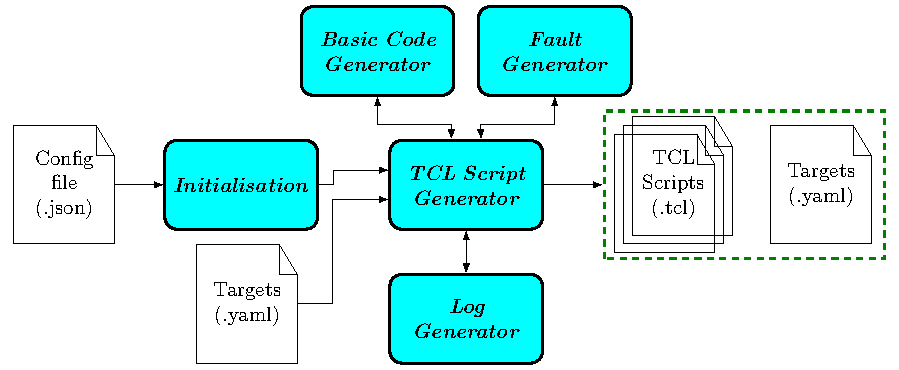
\includegraphics[width=\textwidth]{c4_fissa/img/fissa/archi_tcl_gen.pdf}
    \caption{Software architecture of the TCL Generator module}
    \label{fig:archi_tcl_gen}
\end{figure}

Algorithm~\ref{algo:pseudoCodeSimus} depicts the pseudocode of a simulation of a fault injection, showcasing requirements, and each state with essential parameters. Additionally, the corresponding Python class from Figure~\ref{fig:archi_tcl_gen} is added for each line.
Line 5 in Algorithm~\ref{algo:pseudoCodeSimuStages} corresponds to Algorithm~\ref{algo:pseudoCodeSimus}. This algorithm is executed multiple times with different inputs to build a TCL script.


\begin{algorithm}
    \caption{FIA simulation pseudocode}
    \label{algo:pseudoCodeSimus}
    \normalsize
    \begin{algorithmic}[1]
        \Require $target$
        \Require $cycle$
        \Require $fault$\textunderscore$model$
        \State $tcl$\textunderscore$script = init$\textunderscore$sim(fault$\textunderscore$model, cycle, target)$ \textcolor{blue}{\scriptsize // generated by Basic Code Generator}
        \State $tcl$\textunderscore$script += inject$\textunderscore$fault(fault$\textunderscore$model)$  \textcolor{red}{\scriptsize // generated by Fault Generator}
        \State $tcl$\textunderscore$script += run$\textunderscore$sim()$ \textcolor{blue}{\scriptsize // generated by Basic Code Generator}
        \State $tcl$\textunderscore$script += log$\textunderscore$sim(fault$\textunderscore$model)$ \textcolor{ForestGreen}{\scriptsize // generated by Log Generator}
        \State $tcl$\textunderscore$script += end$\textunderscore$sim()$ \textcolor{blue}{\scriptsize // generated by Basic Code Generator}
        \State $tcl$\textunderscore$file.write(tcl$\textunderscore$script)$ \textcolor{black}{\scriptsize // append and write the simulation data inside the TCL file}
    \end{algorithmic}
\end{algorithm}

%%%%%%%%%%%%%%%%%%%%%%%%%%%%%%%%%%%%%%%%%%
\subsection{Fault Injection Simulator}
\label{subsec:FIS}

The \textit{Fault Injection Simulator} mainly relies on an existing HDL simulator to perform simulations by executing the TCL scripts produced by the \textit{TCL generator}. The log files, in JSON format, are generated by the TCL script for each simulation.
This file encompasses data such as the current simulation number, the executed clock cycle count, the values of the targets' file, the targets faulted, the fault model and the end-of-simulation status.

Listing~\ref{code:logJSONFile_fissa} shows a simplified example of an output file from a simulation. Many lines are omitted to simplify the text and its comprehension. In this example, we have the result of the first simulation of the campaign. The fault model is a single bit-flip in one target at a given clock cycle, and the target, which is a register in this case, \texttt{pc\_id\_o\_tag}, has a size of one bit. A fault has been injected at the period time of \SI{137140}{\nano\second}. The omitted lines, at line 7, include all registers from the register file, all register file tags, and all registers from the target list. The last line, line 14, shows that this simulation ended with a status equal to 3 (i.e., exception delayed from the reference simulation).

\begin{figure}[ht]
    \centering
    \includegraphics[width=.5\textwidth, page=4]{c4_fissa/img/fissa/archi_fissa.pdf}
    \caption{Fault Injection Simulator architecture}
    \label{fig:archi_fis}
\end{figure}

It is worth noting that the set of calls to the generated TCL scripts has to be integrated into the designer's existing design flow, allowing the design compilation, initialisation, and management of input stimuli. The use of TCL scripts simplifies such an integration. 
Once all the fault injection simulations have been performed, the log files can be sent to the \textit{Analyser} which, is described in the following subsection.

\begin{lstlisting}[style=topPosition, language=json, label=code:logJSONFile_fissa, caption=Extract of an example of a FISSA output log JSON file]
"simulation_1": {
    "cycle_ref": 100,
    "cycle_ending": 4,
    "TPR": "32'h0000a8a2",
    "TCR": "32'h00341800",
    "rf1": "32'h000006fc",
    (...)
    "faulted_register": "/tb/top_i/core_region_i/RISCV_CORE/if_stage_i/pc_id_o_tag",
    "size_faulted_register": 1,
    "threat": "bitflip",
    "bit_flipped": 0,
    "cycle_attacked": "137140 ns",
    "simulation_end_time": "137300 ns",
    "status_end": 3
}\end{lstlisting}

%%%%%%%%%%%%%%%%%%%%%%%%%%%%%%%%%%%%%%%%%%
\subsection{Analyser}
\label{subsec:analyser}

The \textit{Analyser} reads all log files and generates a set of \LaTeX~tables (\textit{.tex} files) and/or sensitivity heatmaps (in PDF format) according to the fault models, allowing the user to identify the sensitive hardware elements in the circuit design. 
The generated tables can be customised through modification in the \textit{Analyser} Python code.
The current configuration captures and counts the diverse end-of-simulation status.
Heatmaps are generated for multi-target fault models. For instance, when considering a 2 faults scenario disturbing two hardware elements, a 2-dimension heatmap allows the user to identify sensitive couples of hardware elements leading to a potential vulnerability.
Their configuration can be adapted by modifying the \textit{Analyser} Python code. Heatmaps generation is based on \textit{Seaborn}~\cite{seaborn} which relies on \textit{Matplotlib}~\cite{matplotlib}. This library provides a high-level interface for drawing attractive and informative statistical graphics and save them in different formats like PDF, PNG, etc.
In the current configuration, heatmaps highlight the targets leading to a specific end-of-simulation status (e.g. a status identified by the designer as a successful attack).
Once the results have been generated, they can easily be inserted into a vulnerability assessment report. 

\begin{figure}[ht]
    \centering
    \includegraphics[width=.5\textwidth, page=5]{c4_fissa/img/fissa/archi_fissa.pdf}
    \caption{Analyser architecture}
    \label{fig:archi_analyser}
\end{figure}

%%%%%%%%%%%%%%%%%%%%%%%%%%%%%%%%%%%%%%%%%%
\subsection{Extending FISSA}

In order to extend FISSA for integrating an additional fault model, some modifications to the \textit{TCL Script Generator}, the \textit{Basic Code Generator}, the \textit{Fault Generator} and \textit{Log Generator} modules are necessary. 
It requires the extension of the \textit{init\_sim}, \textit{inject\_fault} and \textit{log\_sim} functions presented in Algorithm~\ref{algo:pseudoCodeSimus} to implement the new fault model from initialisation to logging. 
For instance, these extensions should define the targets for each simulation, the impact of the injections (set to 0/1, bit-flip, random, etc) and the set of data to be logged for this fault model.
The \textit{Log Generator} automates the extraction of specific segments from the ongoing simulation. However, it is customisable, enabling the modification of logged elements, such as incorporating memory content or a list of signals.

\textit{Analyser} can be extended to produce additional \LaTeX~tables, heatmaps or any other way of results visualisation. This can be achieved by either modifying the existing methods or by developing new ones.

An integral aspect of expanding FISSA involves adjusting functions depending on the used HDL simulator. Despite the definition of the TCL language, specific commands vary between simulators. For instance, in Questasim, injecting a fault into a target can be accomplished with the command: “\textit{force \textless object\_name\textgreater \textless value\textgreater -freeze -cancel \textless time\_info\textgreater}”~\cite{modelsim-force}, whereas in Vivado, the equivalent command is: “\textit{add\_force \textless hdl\_object\textgreater \textless values\textgreater -cancel\_after \textless time\_info\textgreater}”~\cite{vivado-force}.
There are some subtle differences between these two software applications that need to be taken into consideration in order to extend FISSA. These distinctions may affect the functionality or compatibility, so addressing them is crucial for a successful adaptation.

%%%%%%%%%%%%%%%%%%%%%%%%%%%%%%%%%%%%%%%%%%%%%%%%%%%%%%%%%%%%%%%%%%%%%%%%%%%%%%%%%%%%%%%%%%%%%%%
\section{Use case example}
\label{section:exampleApplication_fissa}
This section presents a case study to demonstrate the use of FISSA in real conditions. It focuses on the evaluation of the robustness of the DIFT mechanism integrated in the D-RI5CY processor with the Buffer overflow use case from Section~\ref{section:uses_cases}.

%%%%%%%%%%%%%%%%%%%%%%%%%%%%%%%%%%%%%%%%%%
\subsection{FISSA's configuration}
\label{subsec:tool_config}

This subsection presents FISSA's configuration for the addressed use case. We have defined four end-of-simulation statuses, which will be utilised to automatically generate results tables. Examples of these tables will be provided in Subsection~\ref{subsec:results}.
The initial status is labelled as a \textit{crash} (status 1), indicating that the fault injection has caused a deviation in program flow control, leading the processor to execute instructions different from those expected.
The second status, identified as a \textit{silent} fault (status 2), signifies that a fault has occurred but has not impacted the ongoing simulation behaviour.
Status 3, termed a \textit{delay}, denotes that the fault has delayed the DIFT-related exception, meaning the exception is not raised at the same clock cycle as in the reference simulation.
The last status refers to a \textit{success} (status 4), indicating a bypass of the DIFT mechanism and thereby marking a successful attack. This status corresponds to the detection of the end of the simulated program, with no exception being raised.

In the input configuration file, a single injection window is set between cycles 3428 and 3434, the maximum number of simulated clock cycles is set to 100 from the start of the injection window, this allows us to detect if there were a control flow deviation, the design period is set to 40~ns, the number of simulations per TCL script is set to 2,200. The considered fault models are four of the seven fault models defined in Section~\ref{subsec:supported_fault_models}: \textit{target set to 0}, \textit{target set to 1}, \textit{single bit-flip in one target at a given cycle}, and \textit{single bit-flip in two targets at a given cycle}.

Four FIA simulation campaigns are performed to evaluate the design against the four fault models.
We choose to log the values of the \textit{Targets'} file, the simulation's number, targets' value after the injection, the injection cycle and the end-of-simulation status.
The \textit{Targets'} file is filled with the 55 registers of the DIFT security mechanism, representing a total of 127 bits in total.

%%%%%%%%%%%%%%%%%%%%%%%%%%%%%%%%%%%%%%%%%%
\subsection{Experimental results} 
\label{subsec:results}

\begin{figure}[t]
    \centering
    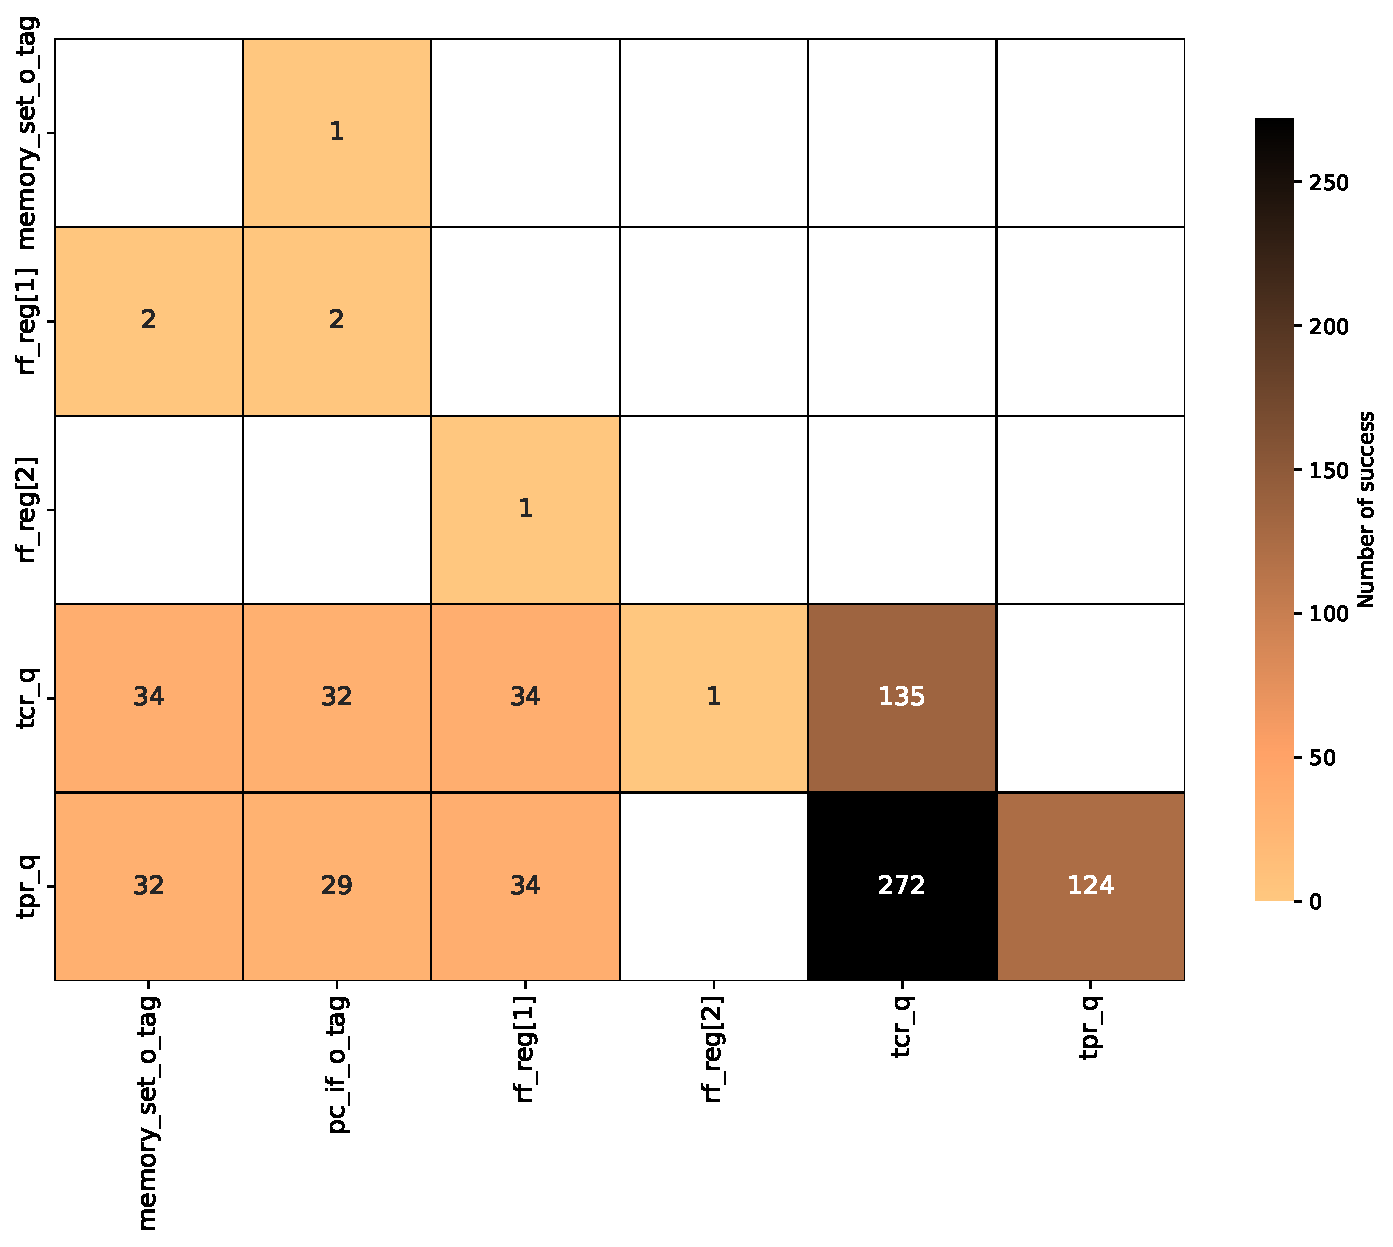
\includegraphics[width=.95\textwidth]{c4_fissa/img/heatmap/heatmap_buffer_overflow_wop_1_single_bitflip_spatial_2.pdf}
    \caption{Extract of the heatmap generated according to the single bit-flip in two targets at a given clock cycle fault model}
    \label{fig:heatmap_spatial}
\end{figure}

This section presents results obtained using FISSA on the considered use case.
All experiments are performed on a server with the following configuration: Xeon Gold 5220 (2,2~GHz, 18C/36T), 128~GB RAM, Ubuntu 20.04.6 LTS and Questasim 10.6e.

Table~\ref{table:end_sim_by_status} summarises the outcomes of the four previously described fault injection campaigns, with each row representing a distinct fault model. Table~\ref{table:end_sim_by_status}'s columns delineate the potential end statuses for each simulation. This table is an essential tool for the designers, enabling them to analyse the vulnerabilities associated with each fault model within their design. Consequently, the designers can determine the necessity for additional protective measures or design alterations.

For instance, Table~\ref{table:end_sim_by_status} illustrates that the '\texttt{set to 1}' fault model results in only three successful outcomes, which represent 0.91\% of the total number of simulations, whereas the '\texttt{single bit-flip in two targets at a given clock cycle}' fault model leads to 1,406 successes, which represent 2.93\% of the total number of simulations. These findings guide the designers in evaluating the significance of protecting against specific fault models.

To further assess vulnerabilities, the designers can utilise Table~\ref{table:end_sim_by_status_wop_1_detail_set0_set1_bitflip}, which provides detailed information on the register and cycle locations of faults for models with fewer successful outcomes. For fault models with multiple registers faulted or with a high number of successes, where the table may become unwieldy, Figure~\ref{fig:heatmap_spatial} serves as a more accessible reference. This figure helps in visualising and interpreting the spatial distribution of vulnerabilities effectively.

\begin{table}
    \centering
    \footnotesize
    \caption{Results of fault injection simulation campaigns}
    \label{table:end_sim_by_status}
    \setlength{\tabcolsep}{3pt}
    \begin{tabular}{@{}rcccccc@{}}
        \toprule
        Fault model                                                        & Crash & Silent  & Delay & Success        & Total   & \begin{tabular}[c]{@{}c@{}}Simulation\\ time\end{tabular} \\
        \midrule
        Set to 0                                                           & 0     & 320     & 1     & 9 (2.73\%)     & 330     & 0h04            \\%\hdashline
        Set to 1                                                           & 0     & 320     & 7     & 3 (0.91\%)     & 330     & 0h04            \\%\hdashline
        Single bit-flip in one target at a given clock cycle               & 0     & 738     & 12    & 12 (1.57\%)    & 762     & 0h11            \\%\hdashline
        Single bit-flip in two targets at a given clock cycle              & 0     & 45,097  & 1,503 & 1,406 (2.93\%) & 48,006  & 13h43           \\%\hdashline
        % \begin{tabular}[c]{@{}r@{}}Single bit-flip in two targets\\ at two different clock cycles\end{tabular}       & 0     & 238,633 & 1,143 & 2,159 (0.89\%) & 241,935 & 42h12           \\\hdashline
        % \begin{tabular}[c]{@{}r@{}}Exhaustive multi-bits faults in\\ one target at a given clock cycle\end{tabular}  & 0     & 927     & 6     & 3 (0.32\%)     & 936     & 0h08            \\\hdashline
        % \begin{tabular}[c]{@{}r@{}}Exhaustive multi-bits faults\\ in two targets at a given clock cycle\end{tabular} & 0     & 67,072  & 926   & 450 (0.66\%)   & 68,448  & 11h11           \\
        \bottomrule
    \end{tabular}
\end{table}

\begin{table*}[t]
    \centering
    \footnotesize
    \caption{Buffer overflow: success per register, fault type and simulation time}
    \label{table:end_sim_by_status_wop_1_detail_set0_set1_bitflip}
    \setlength{\tabcolsep}{1pt}
    \begin{tabular}{@{}rccccccccccccccc@{}}
        \toprule
                                        & \multicolumn{3}{c}{Cycle 3428}                & \multicolumn{3}{c}{Cycle 3429}             & \multicolumn{3}{c}{Cycle 3430} & \multicolumn{3}{c}{Cycle 3431} & \multicolumn{3}{c}{Cycle 3432}                                                                                                                 \\\cmidrule(lr){2-4}\cmidrule(lr){5-7}\cmidrule(lr){8-10}\cmidrule(lr){11-13}\cmidrule(lr){14-16}
                                        & set 0          & set 1          & bit-flip       & set 0          & set 1          & bit-flip    & set 0          & set 1 & bit-flip    & set 0          & set 1 & bit-flip    & set 0          & set 1 & bit-flip    \\
        \midrule
        pc\_if\_o\_tag                  &               &               &               &               &               &            &            &      &            & \checkmark &      & \checkmark &            &      &            \\
        memory\_set\_o\_tag             &               & \checkmark    & \checkmark    &               &               &            &            &      &            &            &      &            &            &      &            \\
        rf\_reg[1]                      &               &               &               &               &               &            & \checkmark &      & \checkmark &            &      &            &            &      &            \\
        tcr\_q                          & \checkmark    &               &               & \checkmark    &               &            & \checkmark &      &            & \checkmark &      &            & \checkmark &      &            \\
        \rowcolor{LightGray} tcr\_q[21] &               &               & \checkmark    &               &               & \checkmark &            &      & \checkmark &            &      & \checkmark &            &      & \checkmark \\
        tpr\_q                          & \checkmark    & \checkmark    &               & \checkmark    & \checkmark    &            &            &      &            &            &      &            &            &      &            \\
        \rowcolor{LightGray} tpr\_q[12] &               &               & \checkmark    &               &               & \checkmark &            &      &            &            &      &            &            &      &            \\
        \rowcolor{LightGray} tpr\_q[15] &               &               & \checkmark    &               &               & \checkmark &            &      &            &            &      &            &            &      &            \\
        \bottomrule
    \end{tabular}
\end{table*}

Table~\ref{table:end_sim_by_status_wop_1_detail_set0_set1_bitflip} is produced by FISSA and details the successes from three distinct fault injection campaigns: \texttt{set to 0}, \texttt{set to 1} and \texttt{single bit-flip in one target at a given cycle}. Table~\ref{table:end_sim_by_status_wop_1_detail_set0_set1_bitflip} specifies successes for each fault model, correlated with the cycle and the affected target. For example, a \texttt{set to 0} fault at cycle 3428 on \texttt{tcr\_q} would lead to a successfully attack. It highlights which targets are sensitive to fault attacks at a cycle-accurate and bit-accurate level, providing the designers precise information on critical elements requiring protection based on their specific needs.  Table~\ref{table:end_sim_by_status_wop_1_detail_set0_set1_bitflip} only covers the most basic fault models. Indeed, producing a table for more complex scenarios, such as simultaneous faults in two targets within a same or multiple cycles, would be intricate and challenging to interpret. Consequently, we opted for an alternative method and developed a heatmap representation (e.g. Figure~\ref{fig:heatmap_spatial}).

To further explore the impact of FIA on a design, a designer can study heatmaps generated by FISSA. 
These heatmaps are tailored to a fault model with two faulty registers, where each matrix intersection shows the number of successes with that target pair.

Figure~\ref{fig:heatmap_spatial} shows an extract of the heatmap generated for the \textit{single bit-flip in two targets at a given clock cycle} fault model. For simplicity, only 5 registers are represented. The full figure will be presented in Chapter~\ref{chapter:exp_setup_results}.
The colour scale represents the number of fault injections targeting a couple of hardware elements (i.e. registers for this use case) leading to a \textit{success} as defined in Subsection~\ref{subsec:tool_config}. We can note that this colour scale, in our case, range from 0 to 272.
This figure highlights the registers that are critical to a specific fault model, enabling the designer to evaluate the design and determine where protection is needed and at what level. It provides a clear indication of which areas require minimal protection and which ones demand a very high level of security. All of this information allow the designer to prioritise countermeasures according to allocated budget, protection requirements, etc.
To give an example, it can be noted that the horizontally displayed registers \texttt{tcr\_q} and \texttt{tpr\_q} are critical registers, because a success will occur regardless of the associated register. Similarly, the registers shown vertically, \texttt{memory\_set\_o\_tag}, \texttt{pc\_if\_o\_tag}, and \texttt{rf\_reg[1]}, are also critical because they lead to many successes with almost all tested registers.

To provide an analytical perspective from the buffer overflow use case presented in Section~\ref{section:uses_cases}, the five previously mentioned registers are critical as they either store the DIFT security policy configuration (\texttt{tpr\_q} and \texttt{tcr\_q}) or store (\texttt{rf\_reg[1]} represents the tag associated with the value of the Program Counter (PC), which is stored in the register file at index 1 for RISC-V ISA) and propagate the tag (\texttt{pc\_if\_o\_tag}) associated with the PC. This is particularly important in our example, which demonstrates a ROP attack with a buffer overflow.
The colour scale indicates the impact of the fault injections on the combination of registers tested. For example, a pair associated with a high number such as 272, 124, and 135 for \texttt{tcr\_q} and \texttt{tpr\_q} are very high priority as they lead to 37.77\% success on this fault model (i.e. with all registers taken into account, see Table~\ref{table:end_sim_by_status}).
In addition, we can see that a register produce a low number of successes, such as \mbox{\texttt{rf\_reg[2]}}; this register is then not the highest priority for protection for the designer.

While Table~\ref{table:end_sim_by_status} provides the total number of \textit{successes} for each fault model and Table~\ref{table:end_sim_by_status_wop_1_detail_set0_set1_bitflip} gives the successes for each fault model (\textit{set to 0}, \textit{set to 1}, and \textit{a single bit flip in a target at a given cycle}) correlated with the cycle and affected target, Figure~\ref{fig:heatmap_spatial} shows that fault injections in 246 register pairs result in a \textit{success}. This information allows the designer to focus on specific simulation traces to understand the effect(s) of the fault(s) and improve the robustness of his design by implementing adapted countermeasures.

%%%%%%%%%%%%%%%%%%%%%%%%%%%%%%%%%%%%%%%%%%%%%%%%%%%%%%%%%%%%%%%%%%%%%%%%%%%%%%%%%%%%%%%%%%%%%%%
\section{Discussion and Perspectives}

In this section, we will discuss this proposed tool and draw some perspectives for the long-term development.
In terms of execution time, we did in total around 24,000,000 simulations for approximatively 3 seconds for each simulation in average spanning from initialisation to data recording.
The execution time is contingent upon various parameters, including the design's size, the specific simulation case, and the number of targets involve.
Actual FIAs are faster than simulations, taking about 0.35 seconds per injection in our tests, relying on the ChipWhisperer-lite platform for clock glitching injection.
While simulations may be slower, they offer the benefit of not requiring an FPGA prototype or the final circuit. Furthermore, it allows integrating vulnerability assessment in the first stages of the development flow and provides a rich set of information for the designer in order to understand sources of vulnerabilities in his design.

As perspectives, we plan to extend FISSA to support new fault models and HDL simulators such as Vivado or Verilator.
Additionally, we intend to enhance integration into the design workflow by adding more automatisation. This may include the management of HDL sources compilation, design's input stimuli or the development of a graphical user interface to improve the overall user experience.
%%%%%%%%%%%%%%%%%%%%%%%%%%%%%%%%%%%%%%%%%%%%%%%%%%%%%%%%%%%%%%%%%%%%%%%%%%%%%%%%%%%%%%%%%%%%%%%
\section{Summary}
In this chapter, we presented FISSA (Fault Injection Simulation for Security Assessment), our advanced and versatile open-source tool designed to automate fault injection campaigns. FISSA is engineered to seamlessly integrate with renowned HDL simulators, such as Questasim. It facilitates the execution of simulations by generating TCL scripts and produces comprehensive JSON log files for subsequent security analysis.

FISSA empowers designers to evaluate their designs during the conceptual phase by allowing them to select specific assessment parameters, including the fault model and target components, tailored to their unique requirements. The insights gained from the results generated by this tool enable designers to enhance the security of their designs, thus adhering to the principles of \textit{Security by Design}.


%%%%%%%%%%%%%%%%%%%%%%%%%%%%%%%%%%%%%%%%%%%%%%%%%%%%%%%%%%%%%%%%%%%%%%%%%%%%%%%%%%%%%%%%%%%%%%%

\clearemptydoublepage
\chapter{Error Detection and Correction Codes to Protect an In-Core DIFT against FIAs}
\chaptermark{Error Detection and Correction codes to protect an In-Core DIFT against FIAs}
\label{chapter:countermeasures}
\minitoc

%%%%%%%%%%%%%%%%%%%%%%%%%%%%%%%%%%%%%%%%%%%%%%%%%%%%%%%%%%%%%%%%%%%%%%%%%%%%%%%%%%%%%%%%%%%%%%%
\section{Introduction}
Previous chapters have shown that the D-RI5CY's DIFT security mechanism is vulnerable to fault injection attacks, mainly due to single-bit flips. This D-RI5CY essentially uses single-bit registers, as it relies on 1-bit tags.

In this chapter, we present three countermeasures in order to protect the DIFT against FIAs.
The first countermeasure implemented to detect and prevent the use of corrupted data is simple parity. We selected the simple parity code as the error detection countermeasure because of its suitability and limited overhead. However, parity codes are limited in that they can only detect, but not correct, single-bit errors.
The second countermeasure is implemented to detect any single-bit errors that may occur, but also to correct them without time overhead. With this countermeasure, we want to correct to the nearest cycle so that the fault cannot propagate and show to a potential attacker that the fault he injected had no effect on the system.
The third countermeasure is called SECDED for Single Error Correction, Double Error Detection. This protection is a Hamming Code extended with a single parity bit to allow the detection of double-bit errors while being able to correct single-bit errors.
This chapter presents the work done during a 4-month research stay, funded by the \textit{Collège Doctoral de Bretagne}, \textit{GDR ISIS (CNRS)}, and the \textit{Université Bretagne Sud}, within the \textit{ALaRI} laboratory (\textit{Advanced Learning and Research Institute}) in the \textit{Università della Svizzera Italiana} in Lugano, Switzerland.
This work has been published in ISVLSI 2024~\cite{PRLG-24-isvlsi}.

The first section presents the different considered fault models. Then, the second section presents simple parity and details its implementation. Afterwards, the third section presents Hamming Code principles, with a simple example, and details our implementation. The fourth section presents SECDED with an example and gives an overview on our implementation. Finally, we discuss these countermeasures and compare them.

%%%%%%%%%%%%%%%%%%%%%%%%%%%%%%%%%%%%%%%%%%%%%%%%%%%%%%%%%%%%%%%%%%%%%%%%%%%%%%%%%%%%%%%%%%%%%%%
\section{Fault models considered in this chapter}
In Chapter~\ref{chapter:dift_assessment}, we assessed the D-RI5CY design by considering \textit{single bit-flip in one register at a given clock cycle}, \textit{bit reset}, and \textit{bit set} fault models. The conclusion of this chapter was that the D-RI5CY is vulnerable mostly to single bit-flip, due to the fact that this DIFT design is mostly built around 1-bit registers for tag propagation.

In this chapter, we consider an attacker able to inject faults into DIFT-related registers, leading to single bit-flips at any position of the targeted register. To reach this objective, any DIFT-related register maintaining 1-bit tag value, driving the tag propagation or the tag update process or maintaining the security policy configuration can be targeted. Studies presented in~\cite{ZDCRT-12-dcis,CLFT-14-cosade} have shown that such precise single bit-flip attacks targeting registers can be performed using, for example, laser shots. We also consider an attacker able to inject a \textit{single bit-flip in two registers at two distinct clock cycles}, with a minimum delay of one clock cycle. Nowadays, more and more platforms exist to perform multi-bits faults on different targets~\cite{alphanov-doubleLFI,alphanov-fourLFI}. These platforms are helping to spread the use of this type of attack, thus we should also be forging our protection around these kinds of threats.

\begin{table}
    \centering
    \small
    \caption{D-RI5CY Registers Details List}
    \label{tab:driscy_register_info}
    \begin{tabular}{rlcc}
        \toprule
        Register Name                   & Module                                            & Size & Group \\
        \midrule
        pc\_id\_o\_tag                  & \textcolor{red}{Instruction Fetch Stage}          & 1    & Gr5   \\
        pc\_if\_o\_tag                  & \textcolor{red}{Instruction Fetch Stage}          & 1    & Gr5   \\\hdashline
        alu\_operand\_a\_ex\_o\_tag     & \textcolor{blue}{Instruction Decode Stage}        & 1    & Gr5   \\
        alu\_operand\_b\_ex\_o\_tag     & \textcolor{blue}{Instruction Decode Stage}        & 1    & Gr5   \\
        alu\_operand\_c\_ex\_o\_tag     & \textcolor{blue}{Instruction Decode Stage}        & 1    & Gr5   \\
        alu\_operator\_o\_mode          & \textcolor{blue}{Instruction Decode Stage}        & 2    & Gr5   \\
        check\_d\_o\_tag                & \textcolor{blue}{Instruction Decode Stage}        & 1    & Gr5   \\
        check\_s1\_o\_tag               & \textcolor{blue}{Instruction Decode Stage}        & 1    & Gr5   \\
        check\_s2\_o\_tag               & \textcolor{blue}{Instruction Decode Stage}        & 1    & Gr5   \\
        is\_store\_post\_o\_tag         & \textcolor{blue}{Instruction Decode Stage}        & 1    & Gr5   \\
        memory\_set\_o\_tag             & \textcolor{blue}{Instruction Decode Stage}        & 1    & Gr5   \\
        regfile\_alu\_waddr\_ex\_o\_tag & \textcolor{blue}{Instruction Decode Stage}        & 5    & Gr4   \\
        register\_set\_o\_tag           & \textcolor{blue}{Instruction Decode Stage}        & 1    & Gr5   \\
        store\_dest\_addr\_ex\_o\_tag   & \textcolor{blue}{Instruction Decode Stage}        & 1    & Gr5   \\
        store\_source\_ex\_o\_tag       & \textcolor{blue}{Instruction Decode Stage}        & 1    & Gr5   \\
        use\_store\_ops\_ex\_o          & \textcolor{blue}{Instruction Decode Stage}        & 1    & Gr5   \\\hdashline
        rf\_reg[0]                      & \textcolor{LimeGreen}{Register File Tag}          & 1    & Gr3   \\
        rf\_reg[1]                      & \textcolor{LimeGreen}{Register File Tag}          & 1    & Gr3   \\
        rf\_reg[2]                      & \textcolor{LimeGreen}{Register File Tag}          & 1    & Gr3   \\
        \ldots                      & \textcolor{LimeGreen}{Register File Tag}          & \ldots    & Gr3   \\
        rf\_reg[30]                     & \textcolor{LimeGreen}{Register File Tag}          & 1    & Gr3   \\
        rf\_reg[31]                     & \textcolor{LimeGreen}{Register File Tag}          & 1    & Gr3   \\\hdashline
        rs1\_o\_tag                     & \textcolor{DarkOrange}{Execute Stage}             & 1    & Gr5   \\\hdashline
        tcr\_q                          & \textcolor{DarkRed}{Control and Status Registers} & 32   & Gr1   \\
        tpr\_q                          & \textcolor{DarkRed}{Control and Status Registers} & 32   & Gr2   \\\hdashline
        data\_type\_q\_tag              & \textcolor{magenta}{Load/Store Unit}              & 2    & Gr5   \\
        data\_we\_q\_tag                & \textcolor{magenta}{Load/Store Unit}              & 1    & Gr5   \\
        rdata\_offset\_q\_tag           & \textcolor{magenta}{Load/Store Unit}              & 2    & Gr5   \\
        rdata\_q\_tag                   & \textcolor{magenta}{Load/Store Unit}              & 4    & Gr5   \\
        \bottomrule
    \end{tabular}
\end{table}
    

%%%%%%%%%%%%%%%%%%%%%%%%%%%%%%%%%%%%%%%%%%%%%%%%%%%%%%%%%%%%%%%%%%%%%%%%%%%%%%%%%%%%%%%%%%%%%%%
\section{Simple Parity}
\label{chapter:simpleparity}

Parity codes represent one of the simplest and most fundamental methods for error detection in digital communication systems. Utilised across a wide range of applications, parity codes help to ensure data integrity by adding a single parity bit to a block of data. This bit acts as a basic error-detection mechanism, enabling the identification of single-bit errors during transmission. Parity codes are commonly classified into two types: even parity and odd parity. In an even parity system, the parity bit is set such that the total number of 1s in the data block, including the parity bit, is even. Conversely, in an odd parity system, the parity bit is adjusted so that the number of \texttt{1} is odd.

%%%%%%%%%%%%%%%%%%%%%%%%%%%%%%
\subsection{Simple parity in a nutshell}
The key advantage of parity codes lies in their simplicity and low overhead. A single parity bit, added to each data block, is sufficient to detect any single-bit error in the block. This one bit stores the parity of the initial message. Figure~\ref{fig:simpleparity_functionning} shows how the data, in blue, and the parity bit, in red, are associated to form an encoded data.

\begin{figure}[ht]
    \centering
    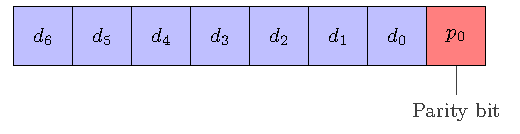
\includegraphics[page=1]{c5_countermeasures_dift/img/simple_parity.pdf}
    \caption{Simple Parity -- functioning}
    \label{fig:simpleparity_functionning}
\end{figure}

Equation~\ref{equat:simpleparity} shows how the parity bit is computed. Each bit of the initial message is XOR'd to calculate parity.

\begin{equation} \label{equat:simpleparity}
    \begin{split}
        p_{0} &= d_{0} \oplus d_{1} \oplus d_{2} \oplus d_{3} \oplus d_{4} \oplus d_{5} \oplus d_{6}
    \end{split}
\end{equation}

Figures~\ref{fig:simpleparity_example_1} and \ref{fig:simpleparity_example_2} show an example of a message with its parity bit. The message is \texttt{0b1001101}. Hence, as there is an even number of '\texttt{1}', the parity bit is set to '\texttt{0}'.

\begin{figure}[ht]
    \centering
    \begin{subfigure}[b]{0.49\textwidth}
        \includegraphics[width=\textwidth, page=2]{c5_countermeasures_dift/img/simple_parity.pdf}
        \caption{Initial message}
        \label{fig:simpleparity_example_1}
    \end{subfigure}
    \hfill
    \begin{subfigure}[b]{0.49\textwidth}
        \includegraphics[width=\textwidth, page=3]{c5_countermeasures_dift/img/simple_parity.pdf}
        \caption{Message with its parity bit}
        \label{fig:simpleparity_example_2}
    \end{subfigure}
    \hfill
    \begin{subfigure}[b]{0.49\textwidth}
        \includegraphics[width=\textwidth, page=4]{c5_countermeasures_dift/img/simple_parity.pdf}
        \caption{Single-bit fault inside the message}
        \label{fig:simpleparity_faulted_example_3}
    \end{subfigure}
    \hfill
    \begin{subfigure}[b]{0.49\textwidth}
        \includegraphics[width=\textwidth, page=5]{c5_countermeasures_dift/img/simple_parity.pdf}
        \caption{Two single-bit faults inside the message}
        \label{fig:simpleparity_faulted_example_4}
    \end{subfigure}
    \caption{Example of a simple parity calculation and its fault detection capacity}
    \label{fig:simpleparity_example}
\end{figure}

Figures~\ref{fig:simpleparity_faulted_example_3} and \ref{fig:simpleparity_faulted_example_4} present, respectively, two examples of when a fault occurs and when two faults happen.
In the first example, Figure~\ref{fig:simpleparity_faulted_example_3}, the bit $d_2$ (from Figure~\ref{fig:simpleparity_functionning}), in red, is faulted. As the faulted message is \texttt{0b1001001}, it means that the new calculated parity bit value should be \texttt{1}. Hence, the fault will be detected as the parity bit differs from the original computed message (Figure~\ref{fig:simpleparity_example_2}).
In the second case, two faults happen in the message at bits $d_2$ and $d_5$ (from Figure~\ref{fig:simpleparity_functionning}). So, the faulted message is \texttt{0b1101001}, then, when the new parity bit is calculated, the parity bit value will not change as there is still an even number of \texttt{1} compared to the initial message. This shows the limitation of this error detection code.

%%%%%%%%%%%%%%%%%%%%%%%%%%%%%%
\subsection{Implementation: Minimisation of redundancy bits}

In order to implement simple parity, we decided, in a first approach, to optimise the number of parity bits. We had different choices, but we decided to form five groups. These groups are composed of one or more register according to their criticality. Table~\ref{tab:driscy_register_info} presents all 55 registers of the D-RI5CY mechanism with their size (in number of bits) and the group in which they are associated with. Each colour represents a different HDL module.
Firstly, the two registers that contain the security policy, TCR and TPR, are highly critical. As a result, we have chosen to form a separate group for each of them. Although these registers are 32 bits long, only 22 bits are fully utilised in the current implementation, making bits 22 to 31 unnecessary. Therefore, we have decided not to protect these unused bits or include them in parity calculations.
Secondly, the third logical group consists of keeping the 32 registers of the register file tag together. Since these registers are already grouped, it makes sense to maintain this grouping.
This leaves us with one 5-bit register, sixteen 1-bit registers, three 2-bit registers, and one 4-bit register. The 5-bit register is used to store the tag destination address, which is critical. As such, we have decided to create a dedicated group for it. The remaining 20 registers, which total 26 bits, are combined into a fifth group.
Table~\ref{tab:sp_group} shows the five groups formed to implement the protection for 107 bits in total. One parity bit protects each group.

\begin{table}[t]
    \centering
    \footnotesize
    \caption{DIFT-related protected registers -- simple parity}
    \label{tab:sp_group}
    \begin{tabular}{@{}ccccc@{}}
        \toprule
                & Protected register                                                                                & \begin{tabular}[c]{@{}c@{}}Number of\\ bits\end{tabular} & \begin{tabular}[c]{@{}c@{}}Number of\\ protected bits\end{tabular} & \begin{tabular}[c]{@{}c@{}}Number of\\ parity bits\end{tabular} \\ \midrule
        Group 1 & TCR                                                                                               & 32                                                       & 22                                                                 & 1                                                               \\
        Group 2 & TPR                                                                                               & 32                                                       & 22                                                                 & 1                                                               \\
        Group 3 & Register File Tag                                                                               & 32                                                       & 32                                                                 & 1                                                               \\
        Group 4 & Tag destination address                                                                           & 5                                                        & 5                                                                  & 1                                                               \\
        Group 5 & \begin{tabular}[c]{@{}c@{}}16×1-bit registers\\ 3×2-bit registers\\ 1×4-bit register\end{tabular} & 26                                                       & 26                                                                 & 1                                                               \\ \midrule
        Total   &                                                                                                   & 127                                                      & 107                                                                & 5                                                               \\
        \bottomrule
    \end{tabular}
\end{table}

Figure~\ref{fig:implementation_sp} presents our proposed implementation for the simple parity. This implementation is straightforward. To protect a register (shown in blue), the input is directed simultaneously to both the protected register and an encoder (in green). The encoder calculates the parity using combinatorial logic, storing the resulting parity bit in a separate register, depicted in salmon-red in the figure. The parity bit is stored in this register during the same cycle as the input value is stored in the protected register. Subsequently, the decoder computes the parity of the protected register and compares it with the parity bit stored in the parity bit register. If a difference is detected, it indicates the injection of a fault, which causes an alert signal to be raised.

\begin{figure}[ht]
    \centering
    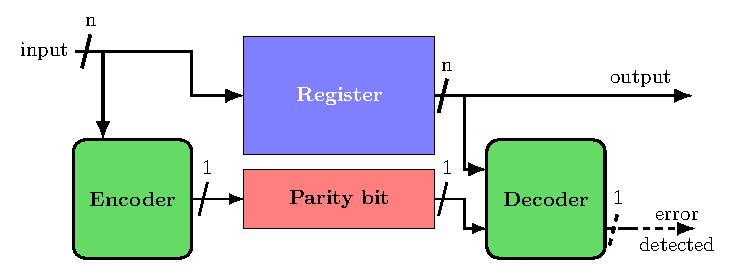
\includegraphics[page=1]{c5_countermeasures_dift/img/archi_contremesures.pdf}
    \caption{Implementation of simple parity}
    \label{fig:implementation_sp}
\end{figure}

%%%%%%%%%%%%%%%%%%%%%%%%%%%%%%%%%%%%%%%%%%%%%%%%%%%%%%%%%%%%%%%%%%%%%%%%%%%%%%%%%%%%%%%%%%%%%%%
\section{Hamming Codes}
\label{chapter:hammingcode}

In digital communication and error correction theory, Hamming Codes represent a pioneering development in ensuring data integrity during transmission over unreliable channels. Developed by Richard Hamming in 1950~\cite{H-50-bstj}, this class of error-correcting codes is designed to detect and correct single-bit errors and detect, without the correction part, two-bit errors. The Hamming Code is a linear block code that enhances data transmission reliability by introducing redundancy in a structured manner.

The importance of Hamming Codes lies not only in their ability to maintain the integrity of data but also in their efficiency relative to other early error correction schemes. As such, Hamming Codes have found wide application in areas where high data accuracy is required, such as computer memory systems, telecommunications, and satellite communication. Despite the emergence of more sophisticated error-correcting codes in modern systems, the simplicity and effectiveness of Hamming Codes make them a foundational topic in the study of error correction algorithms.

%%%%%%%%%%%%%%%%%%%%%%%%%%%%%%
\subsection{Hamming Code in a nutshell}

\begin{figure}[ht]
    \centering
    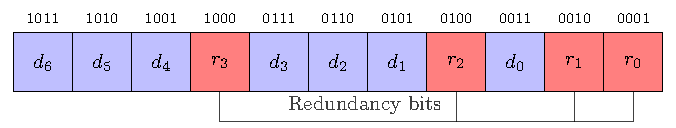
\includegraphics[page=1]{c5_countermeasures_dift/img/hamming_bit.pdf}
    \caption{Hamming Code (11,7) -- functioning}
    \label{fig:hamming_functionning}
\end{figure}

The fundamental principle behind the Hamming Code is the strategic insertion of $r$ redundancy bits at specific positions within a data block of $d$ bits, such that \(2^r \geqslant d + r + 1\).
These parity bits are used to perform checks on subsets of data bits, allowing the receiver to identify and, in certain cases, correct erroneous bits. The placement and calculation of the parity bits follow a binary positional system (1, 2, 4, 8, 16, \ldots), which forms the core of the error detection and correction mechanism. For example, for an 8-bit word it needs four redundancy bits while for a 64-bit word, it needs only 7 redundancy bits. By positioning the redundancy bits at the indexes of powers of two, it is then possible to correct an error if one is detected. Thus, for example, Hamming Code (11,7) owns seven bits of data ($d_{0}-d_{6}$) and four redundancy bits ($r_{0}-r_{3}$). Data bits and redundancy bits are placed according to Figure~\ref{fig:hamming_functionning}. The most common Hamming Code is the (7,4), which uses four data bits and three redundancy bits.
For the Hamming Code (11,7) (Figure~\ref{fig:hamming_functionning}), redundancy bits are computed according to Equation~\ref{equat:hamming_encoder}. This equation calculation is also represented in Figure~\ref{fig:hamming_code_example}. For example, if the initial message to be sent is \texttt{0b1001101} in binary, the redundancy bit $r_0$ will be computed as $r_0 = d_{0} \oplus d_{1} \oplus d_{3} \oplus d_{4} \oplus d_{6}$. Thus, $r_0$ will be equals to \texttt{1} as depicted in Figure~\ref{fig:hamming_code_example_2}. It is worth noting that this code is not fully used, because with four redundancy bits, Hamming Code is able to protect up to eleven data bits to form Hamming Code (15,11).

\begin{equation} \label{equat:hamming_encoder}
    \begin{split}
        r_{0} = d_{0} \oplus d_{1} \oplus d_{3} \oplus d_{4} \oplus d_{6} \\
        r_{1} = d_{0} \oplus d_{2} \oplus d_{3} \oplus d_{5} \oplus d_{6} \\
        r_{2} = d_{1} \oplus d_{2} \oplus d_{3} \\
        r_{3} = d_{4} \oplus d_{5} \oplus d_{6}
    \end{split}
\end{equation}

\begin{figure}[ht]
    \centering
    \begin{subfigure}[b]{0.49\textwidth}
        \includegraphics[width=\textwidth, page=2]{c5_countermeasures_dift/img/hamming_bit.pdf}
        \caption{Initial message}
        \label{fig:hamming_code_example_1}
    \end{subfigure}
    \hfill
    \begin{subfigure}[b]{0.49\textwidth}
        \includegraphics[width=\textwidth, page=4]{c5_countermeasures_dift/img/hamming_bit.pdf}
        \caption{Calculation of redundancy bit $r_0$}
        \label{fig:hamming_code_example_2}
    \end{subfigure}
    \hfill
    \begin{subfigure}[b]{0.49\textwidth}
        \includegraphics[width=\textwidth, page=6]{c5_countermeasures_dift/img/hamming_bit.pdf}
        \caption{Calculation of redundancy bit $r_1$}
        \label{fig:hamming_code_example_3}
    \end{subfigure}
    \hfill
    \begin{subfigure}[b]{0.49\textwidth}
        \includegraphics[width=\textwidth, page=8]{c5_countermeasures_dift/img/hamming_bit.pdf}
        \caption{Calculation of redundancy bit $r_2$}
        \label{fig:hamming_code_example_4}
    \end{subfigure}
    \hfill
    \begin{subfigure}[b]{0.49\textwidth}
        \includegraphics[width=\textwidth, page=10]{c5_countermeasures_dift/img/hamming_bit.pdf}
        \caption{Calculation of redundancy bit $r_3$}
        \label{fig:hamming_code_example_5}
    \end{subfigure}
    \caption{Hamming Code (11,7) redundancy bits calculations}
    \label{fig:hamming_code_example}
\end{figure}

\begin{equation} \label{equat:hamming_decoder}
    \begin{split}
        nr_{0} = r_{0} \oplus d_{0} \oplus d_{1} \oplus d_{3} \oplus d_{4} \oplus d_{6} = 1 \oplus 1 \oplus 0 \oplus 0 \oplus 0 \oplus 1    = 1 \\
        nr_{1} = r_{1} \oplus d_{0} \oplus d_{2} \oplus d_{3} \oplus d_{5} \oplus d_{6} = 0 \oplus 1 \oplus 1 \oplus 0 \oplus 0 \oplus 1    = 1 \\
        nr_{2} = r_{2} \oplus d_{1} \oplus d_{2} \oplus d_{3}                           = 0 \oplus 0 \oplus 1 \oplus 0                      = 1 \\
        nr_{3} = r_{3} \oplus d_{4} \oplus d_{5} \oplus d_{6}                           = 1 \oplus 0 \oplus 0 \oplus 1                      = 0
    \end{split}
\end{equation}

Figure~\ref{fig:hamming_code_faulted} presents an example of the detection and correction of an error. Figure~\ref{fig:hamming_code_faulted_1} depicts the message sent \texttt{0b10011100101} (1253 in decimal). A fault occurs during the transmission in the bit $d_3$ (Figure~\ref{fig:hamming_code_faulted_2} at position \texttt{0111}). The received message is \texttt{0b10010100101} (1189 in decimal).
During the verification of the redundancy bits. The equation~\ref{equat:hamming_decoder} shows how the new redundancy bits are calculated from the received redundancy and data bits. The association of these new redundancy bits ($nr_{0}-nr_{3}$) is call the syndrome. This syndrome represents the position of the faulted bit and needs to be read backward from $nr_3$ to $nr_0$. As shown in Equation~\ref{equat:hamming_decoder}, the syndrome equals \texttt{0b0111}. This is the correct position of the fault that happened in Figure~\ref{fig:hamming_code_faulted_2}. The same sequence is realised if a fault happens in a redundancy bit. This can be explained as each data bit is checked by at least two redundancy bits, while a redundancy bit is checked only by itself during the decoding phase.

\begin{figure}[ht]
    \centering
    \begin{subfigure}[b]{0.49\textwidth}
        \includegraphics[width=\textwidth, page=11]{c5_countermeasures_dift/img/hamming_bit.pdf}
        \caption{Initial message}
        \label{fig:hamming_code_faulted_1}
    \end{subfigure}
    \hfill
    \begin{subfigure}[b]{0.49\textwidth}
        \includegraphics[width=\textwidth, page=12]{c5_countermeasures_dift/img/hamming_bit.pdf}
        \caption{Injection of a fault in bit $d_3$}
        \label{fig:hamming_code_faulted_2}
    \end{subfigure}
    \hfill
    \begin{subfigure}[b]{0.49\textwidth}
        \includegraphics[width=\textwidth, page=13]{c5_countermeasures_dift/img/hamming_bit.pdf}
        \caption{Calculation of redundancy bit $r_0$}
        \label{fig:hamming_code_faulted_3}
    \end{subfigure}
    \hfill
    \begin{subfigure}[b]{0.49\textwidth}
        \includegraphics[width=\textwidth, page=14]{c5_countermeasures_dift/img/hamming_bit.pdf}
        \caption{Calculation of redundancy bit $r_1$}
        \label{fig:hamming_code_faulted_4}
    \end{subfigure}
    \hfill
    \begin{subfigure}[b]{0.49\textwidth}
        \includegraphics[width=\textwidth, page=15]{c5_countermeasures_dift/img/hamming_bit.pdf}
        \caption{Calculation of redundancy bit $r_2$}
        \label{fig:hamming_code_faulted_5}
    \end{subfigure}
    \hfill
    \begin{subfigure}[b]{0.49\textwidth}
        \includegraphics[width=\textwidth, page=16]{c5_countermeasures_dift/img/hamming_bit.pdf}
        \caption{Calculation of redundancy bit $r_3$}
        \label{fig:hamming_code_faulted_6}
    \end{subfigure}
    \caption{Example of a faulted message with Hamming Code (11,7)}
    \label{fig:hamming_code_faulted}
\end{figure}

%%%%%%%%%%%%%%%%%%%%%%%%%%%%%%
\subsection{Implementation: Minimisation of redundancy bits}

In order to implement Hamming Code, we used the same idea as the previous countermeasure: minimisation of redundancy bits. We used the same five groups as depicted in Table~\ref{tab:hammingcode_group}. As we only protect 22 bits of the 32 bits from TCR and TPR registers, we only need 5 bits of redundancy, instead of 6 bits.

\begin{table}[t]
    \centering
    \footnotesize
    \caption{DIFT-related protected registers -- Hamming Code}
    \label{tab:hammingcode_group}
    \begin{tabular}{@{}ccccc@{}}
        \toprule
                & Protected register                                                                                & \begin{tabular}[c]{@{}c@{}}Number of\\ bits\end{tabular} & \begin{tabular}[c]{@{}c@{}}Number of\\ protected bits\end{tabular} & \begin{tabular}[c]{@{}c@{}}Number of\\ redundancy bits\end{tabular} \\ \midrule
        Group 1 & TCR                                                                                               & 32                                                       & 22  & 5                                                                                                               \\
        Group 2 & TPR                                                                                               & 32                                                       & 22  & 5                                                                                                               \\
        Group 3 & Register File Tag                                                                                 & 32                                                       & 32  & 6                                                                                                               \\
        Group 4 & Tag destination address                                                                           & 5                                                        & 5   & 4                                                                                                               \\
        Group 5 & \begin{tabular}[c]{@{}c@{}}16×1-bit registers\\ 3×2-bit registers\\ 1×4-bit register\end{tabular} & 26                                                       & 26  & 5                                                                                                               \\ \midrule
        Total   &                                                                                                   & 127                                                      & 107 & 25                                                                                                              \\
        \bottomrule
    \end{tabular}
\end{table}

Figure~\ref{fig:implementation_hc_1} presents the proposed implementation for Hamming Code. We do not integrate control signals for clarity. This implementation is straightforward. In order to protect a register or multiples independent registers, we choose to send the input(s) directly to both the protected register(s) (shown in blue) and an encoder. The encoder calculates the different redundancy bits using combinatorial logic, storing the resulting redundancy bits in a separate register, depicted in red in the figure. The redundancy bits are stored in this register at the same cycle as the input(s) value is (are) stored in the protected register(s). Subsequently, the decoder computes the parity of the protected register and compares it with the redundancy bits stored in the redundancy bits register. If a difference is detected, it indicates the injection of a fault, which causes a signal to be sent to indicate the detection. But also, thanks to Hamming Code, we are able to determine where the fault happened and so the decoder will correct the faulted value (dashed arrows). Then this corrected value will be sent to the pipeline, and at the same time, we correct the faulted register.

\begin{figure}[ht]
    \centering
    \includegraphics[page=2, width=\textwidth]{c5_countermeasures_dift/img/archi_contremesures.pdf}
    \caption{Implementation of Hamming Code}
    \label{fig:implementation_hc_1}
\end{figure}

In order to protect the set of 32 1-bit registers from the Register File Tag, we rely on a slightly different approach. Figure~\ref{fig:implementation_hc_2} presents the second approach with six redundancy bits.
We have developed a slightly different approach to minimise the impact on the original design of the D-RI5CY tag register file. Basically, we use the existing two input ports interfaces instead of adding a third input port dedicated to correction. We choose to send the input directly to both the protected register (shown in blue) and an encoder. 
As in the previous case, the decoder allows the detection of an error due to a bit-flip fault in one of the registers. With Hamming Code protection, the decoder produces corrected outputs (dashed arrows) which are propagated to the tag register outputs. If a fault is detected, the corrected output is forwarded to the tag register interface. As soon as one of the two input ports is available, this corrected value is stored in the faulty register to correct the detected fault. A fresh input value has priority on the corrected value to ensure the data flow correctness. 

\begin{figure}[ht]
    \centering
    \includegraphics[page=3, width=\textwidth]{c5_countermeasures_dift/img/archi_contremesures.pdf}
    \caption{Implementation of Hamming Code -- Register File Tag}
    \label{fig:implementation_hc_2}
\end{figure}


%%%%%%%%%%%%%%%%%%%%%%%%%%%%%%%%%%%%%%%%%%%%%%%%%%%%%%%%%%%%%%%%%%%%%%%%%%%%%%%%%%%%%%%%%%%%%%%
\section{Hamming Codes -- SECDED}
\label{section:chap5_secded}

Single Error Correction, Double Error Detection (SECDED) is an error correction technique that enhances the reliability of data transmission and storage, particularly in high-reliability systems. It builds upon the foundation of the Hamming Code by enabling the correction of single-bit errors while also detecting the presence of double-bit errors. This is achieved by adding a global parity bit to the standard Hamming Code structure, allowing the system to distinguish between single and double-bit errors. When a single-bit error is detected, SECDED can automatically correct it, ensuring that data remains intact. In the case of a double-bit error, SECDED can detect it but not correct it, thereby signalling the system to flag the error for further intervention.

SECDED is widely used in critical environments, such as Error-Correcting Code memory systems, where data integrity is paramount, and any data corruption could lead to significant issues. Its ability to detect and correct errors in real time without requiring significant computational resources makes it particularly effective for applications where both reliability and efficiency are required. The additional parity bit adds minimal overhead, making SECDED a practical solution for fault-tolerant systems in sectors like aerospace, telecommunications, and data centres. By balancing error protection and system performance, SECDED ensures that systems can continue to function reliably even in the presence of transient errors.

%%%%%%%%%%%%%%%%%%%%%%%%%%%%%%
\subsection{Single Error Correction, Double Errors Detection in a nutshell}

\begin{figure}[ht]
    \centering
    \includegraphics[page=1]{c5_countermeasures_dift/img/secded.pdf}
    \caption{Hamming Code -- SECDED (12,7) -- principle}
    \label{fig:secded_functionning}
\end{figure}

The fundamental principle behind SECDED compared to Hamming Codes is the addition of an extra bit to calculate the general parity $gp_0$ (Figure~\ref{fig:secded_functionning}). This extra bit works aside of the redundancy bits and helps calculate the parity of the whole message (redundancy bits and data bits). This bit helps detects two bits errors while being able to correct single-bit errors. The parity bit is generally placed at the beginning of the message at index \texttt{0}. As the most common Hamming Code is the (7,4), the most common SECDED code is the (8,4) with four bits of data, three redundancy bits and one parity bit.
Equation~\ref{equat:secded_encoder} presents the calculation of the different redundancy and parity bits for a message of seven data bits.
Figure~\ref{fig:secded_example} also represents the calculation of the general parity bit. This is the same message as for Hamming Codes (Figure~\ref{fig:hamming_code_example_1}), in the previous subsection, so the redundancy bits are already calculated. Figure~\ref{fig:secded_example_1} represents the initial message when all redundancy bits are calculated. If the message with the redundancy bits is equal to \texttt{0b10011100101}, the number of \texttt{1}s is even, then the general parity bit will be set to \texttt{0}, as depicted in Figure~\ref{fig:secded_example_2}.

\begin{equation} \label{equat:secded_encoder}
    \begin{split}
        r_{0}   = d_{0} \oplus d_{1} \oplus d_{3} \oplus d_{4} \oplus d_{6} \\
        r_{1}   = d_{0} \oplus d_{2} \oplus d_{3} \oplus d_{5} \oplus d_{6} \\
        r_{2}   = d_{1} \oplus d_{2} \oplus d_{3} \\
        r_{3}   = d_{4} \oplus d_{5} \oplus d_{6} \\
        gp_{0}  = d_{0} \oplus d_{1} \oplus d_{2} \oplus d_{3} \oplus d_{4} \oplus d_{5} \oplus d_{6} \oplus r_{0} \oplus r_{1} \oplus r_{2} \oplus r_{3}
    \end{split}
\end{equation}

\begin{figure}[ht]
    \centering
    \begin{subfigure}[b]{0.49\textwidth}
        \includegraphics[width=\textwidth, page=2]{c5_countermeasures_dift/img/secded.pdf}
        \caption{Initial message}
        \label{fig:secded_example_1}
    \end{subfigure}
    \hfill
    \begin{subfigure}[b]{0.49\textwidth}
        \includegraphics[width=\textwidth, page=4]{c5_countermeasures_dift/img/secded.pdf}
        \caption{Calculation of general parity bit $gp_0$}
        \label{fig:secded_example_2}
    \end{subfigure}
    \hfill
    \begin{subfigure}[b]{0.49\textwidth}
        \includegraphics[width=\textwidth, page=5]{c5_countermeasures_dift/img/secded.pdf}
        \caption{Final message}
        \label{fig:secded_example_3}
    \end{subfigure}
    \caption{SECDED (12,7) general parity bit calculation}
    \label{fig:secded_example}
\end{figure}

Figure~\ref{fig:secded_faulted_1bit} depicts the injection of a single-bit fault. The received message corresponds to the previous one (\texttt{0b100111001010}). A fault is injected in bit $d_3$ at position \texttt{0111} (seventh position).
The decoder calculation of redundancy bits are done at first in Figures~\ref{fig:secded_faulted_1bit_3}, \ref{fig:secded_faulted_1bit_4}, \ref{fig:secded_faulted_1bit_5}, and \ref{fig:secded_faulted_1bit_6} and then gives the syndrome \texttt{0b0111} for the seventh position which corresponds to the data bit $d_3$. This syndrome is correct. Now, the general parity bit is decoded from all bits of the message in Figure~\ref{fig:secded_faulted_1bit_7}. This time, the general parity bit is not correct (\texttt{1} instead of \texttt{0}). This new value means that a single fault occurred. Because the syndrome and the general parity bit are different of \texttt{0}.

\begin{figure}[ht]
    \centering
    \begin{subfigure}[b]{0.49\textwidth}
        \includegraphics[width=\textwidth, page=5]{c5_countermeasures_dift/img/secded.pdf}
        \caption{Initial message}
        \label{fig:secded_faulted_1bit_1}
    \end{subfigure}
    \hfill
    \begin{subfigure}[b]{0.49\textwidth}
        \includegraphics[width=\textwidth, page=6]{c5_countermeasures_dift/img/secded.pdf}
        \caption{Injection of a fault in bit $d_3$}
        \label{fig:secded_faulted_1bit_2}
    \end{subfigure}
    \hfill
    \begin{subfigure}[b]{0.49\textwidth}
        \includegraphics[width=\textwidth, page=7]{c5_countermeasures_dift/img/secded.pdf}
        \caption{Calculation of redundancy bit $r_0$}
        \label{fig:secded_faulted_1bit_3}
    \end{subfigure}
    \hfill
    \begin{subfigure}[b]{0.49\textwidth}
        \includegraphics[width=\textwidth, page=8]{c5_countermeasures_dift/img/secded.pdf}
        \caption{Calculation of redundancy bit $r_1$}
        \label{fig:secded_faulted_1bit_4}
    \end{subfigure}
    \hfill
    \begin{subfigure}[b]{0.49\textwidth}
        \includegraphics[width=\textwidth, page=9]{c5_countermeasures_dift/img/secded.pdf}
        \caption{Calculation of redundancy bit $r_2$}
        \label{fig:secded_faulted_1bit_5}
    \end{subfigure}
    \hfill
    \begin{subfigure}[b]{0.49\textwidth}
        \includegraphics[width=\textwidth, page=10]{c5_countermeasures_dift/img/secded.pdf}
        \caption{Calculation of redundancy bit $r_3$}
        \label{fig:secded_faulted_1bit_6}
    \end{subfigure}
    \hfill
    \begin{subfigure}[b]{0.49\textwidth}
        \includegraphics[width=\textwidth, page=11]{c5_countermeasures_dift/img/secded.pdf}
        \caption{Calculation of redundancy bit $gp_0$}
        \label{fig:secded_faulted_1bit_7}
    \end{subfigure}
    \caption{Example of a 1 bit fault with SECDED (12,7)}
    \label{fig:secded_faulted_1bit}
\end{figure}

Figure~\ref{fig:secded_faulted_2bits} depicts the injection of a double-bits fault. The received message is still the same (\texttt{0b100111001010}). A fault is injected in bit $d_3$ at position \texttt{0111} (seventh position) and another fault is injected in bit $d_0$ at position \texttt{0011}.
The decoder calculation of redundancy bits are done at first in Figures~\ref{fig:secded_faulted_2bits_3}, \ref{fig:secded_faulted_2bits_4}, \ref{fig:secded_faulted_2bits_5}, and \ref{fig:secded_faulted_2bits_6}, and gives the syndrome \texttt{0b0100} for the fourth position which corresponds to the redundancy bit $r_2$. This syndrome is incorrect and without the general parity bit, Hamming Code would correct the fourth bit, which would lead to the injection of a third fault in the message.
But thanks to SECDED, the general parity bit is decoded from all bits of the message in Figure~\ref{fig:secded_faulted_2bits_7}. This time, the general parity bit is correct (\texttt{0}). This value means that a double fault occurred because the parity did not change while the redundancy bits changed.

\begin{figure}[ht]
    \centering
    \begin{subfigure}[b]{0.49\textwidth}
        \includegraphics[width=\textwidth, page=5]{c5_countermeasures_dift/img/secded.pdf}
        \caption{Initial message}
        \label{fig:secded_faulted_2bits_1}
    \end{subfigure}
    \hfill
    \begin{subfigure}[b]{0.49\textwidth}
        \includegraphics[width=\textwidth, page=12]{c5_countermeasures_dift/img/secded.pdf}
        \caption{Injection of a fault in bit $d_3$ and bit $d_0$}
        \label{fig:secded_faulted_2bits_2}
    \end{subfigure}
    \hfill
    \begin{subfigure}[b]{0.49\textwidth}
        \includegraphics[width=\textwidth, page=13]{c5_countermeasures_dift/img/secded.pdf}
        \caption{Calculation of redundancy bit $r_0$}
        \label{fig:secded_faulted_2bits_3}
    \end{subfigure}
    \hfill
    \begin{subfigure}[b]{0.49\textwidth}
        \includegraphics[width=\textwidth, page=14]{c5_countermeasures_dift/img/secded.pdf}
        \caption{Calculation of redundancy bit $r_1$}
        \label{fig:secded_faulted_2bits_4}
    \end{subfigure}
    \hfill
    \begin{subfigure}[b]{0.49\textwidth}
        \includegraphics[width=\textwidth, page=15]{c5_countermeasures_dift/img/secded.pdf}
        \caption{Calculation of redundancy bit $r_2$}
        \label{fig:secded_faulted_2bits_5}
    \end{subfigure}
    \hfill
    \begin{subfigure}[b]{0.49\textwidth}
        \includegraphics[width=\textwidth, page=16]{c5_countermeasures_dift/img/secded.pdf}
        \caption{Calculation of redundancy bit $r_3$}
        \label{fig:secded_faulted_2bits_6}
    \end{subfigure}
    \hfill
    \begin{subfigure}[b]{0.49\textwidth}
        \includegraphics[width=\textwidth, page=17]{c5_countermeasures_dift/img/secded.pdf}
        \caption{Calculation of redundancy bit $gp_0$}
        \label{fig:secded_faulted_2bits_7}
    \end{subfigure}
    \caption{Example of two 1-bit faults with SECDED (12,7)}
    \label{fig:secded_faulted_2bits}
\end{figure}

\begin{table}[t]
    \centering
    \footnotesize
    \caption{Summarise of the three case for SECDED}
    \label{tab:sumup_secded}
    \begin{tabular}{@{}c|cc@{}}
        \toprule
        Fault Detection         & Redundancy Bits   & General Parity Bit \\\midrule
        No fault                & $\{r_0 - r_3\} = 0$ & $gp_0 = 0$        \\
        Single Error Correction & $\{r_0 - r_3\} \neq 0$                  & $gp_0 = 1$                   \\
        Double Errors Detection & $\{r_0 - r_3\} \neq 0$                  & $gp_0 = 0$                   \\
        \bottomrule
    \end{tabular}
\end{table}

To conclude on SECDED, this code allows correcting single-bit errors and detect double-bit errors in a message. It is a lightweight countermeasure, as it only adds a few redundancy bits and one general parity bit. When a fault occurs, there are three different possible cases represented in Table~\ref{tab:sumup_secded}. In the first case, the syndrome formed by the redundancy bits is equal to \texttt{0} and the general parity bit syndrome is also equal to \texttt{0}, in that case, nothing happened, the message is correct.
In the second case, if the syndrome formed by the redundancy bits is different from \texttt{0} and the general parity bit is equal to \texttt{1}, this means that an error has occurred and the syndrome of the redundancy bits will give its position to allow correction at the correct index.
The third case is represented by a redundancy bits syndrome different from \texttt{0} and a general parity bit equal to \texttt{0}, in that case, it means that a double bits error occurred. This time the error can not be corrected. The limitation of this code is achieved when a three bits error occurs.

%%%%%%%%%%%%%%%%%%%%%%%%%%%%%%
\subsection{Implementation: Minimisation of redundancy bits}

In order to implement SECDED, we used the same idea as the previous countermeasures: minimisation of redundancy bits. We used the same five groups as depicted in Table~\ref{tab:secded_group}. In total, we have to use \compute{25+6}{0} bits to protect our mechanism with SECDED against single-bit errors and double-bit errors.

\begin{table}[t]
    \centering
    \footnotesize
    \caption{DIFT-related protected registers -- SECDED}
    \label{tab:secded_group}
    \begin{tabular}{@{}cccccc@{}}
        \toprule
                & Protected register                                                                                & \begin{tabular}[c]{@{}c@{}}Number of\\ bits\end{tabular} & \begin{tabular}[c]{@{}c@{}}Number of\\ protected bits\end{tabular} & \begin{tabular}[c]{@{}c@{}}Number of\\ redundancy bits\end{tabular} & \begin{tabular}[c]{@{}c@{}}Number of\\ parity bits\end{tabular} \\ \midrule
        Group 1 & TCR                                                                                               & 32                                                       & 22                                                                 & 5                                                                   & 1                                                               \\
        Group 2 & TPR                                                                                               & 32                                                       & 22                                                                 & 5                                                                   & 1                                                               \\
        Group 3 & Register File Tag                                                                                 & 32                                                       & 32                                                                 & 6                                                                   & 1                                                               \\
        Group 4 & Tag destination address                                                                           & 5                                                        & 5                                                                  & 4                                                                   & 1                                                               \\
        Group 5 & \begin{tabular}[c]{@{}c@{}}16×1-bit registers\\ 3×2-bit registers\\ 1×4-bit register\end{tabular} & 26                                                       & 26                                                                 & 5                                                                   & 1                                                               \\ \midrule
        Total   &                                                                                                   & 127                                                      & 107                                                                & 25                                                                  & 5                                                               \\
        \bottomrule
    \end{tabular}
\end{table}

Figure~\ref{fig:implementation_sd_1} and Figure~\ref{fig:implementation_sd_2} present the proposed implementations for SECDED. We do not integrate control signals for clarity in these figures. This is approximatively the same figures as for Hamming Code (Figure~\ref{fig:implementation_hc_1} and Figure~\ref{fig:implementation_hc_2}) but with the representation of the extra register that stores the general parity bit.

\begin{figure}[ht]
    \centering
    \includegraphics[page=4, width=\textwidth]{c5_countermeasures_dift/img/archi_contremesures.pdf}
    \caption{Implementation of SECDED}
    \label{fig:implementation_sd_1}
\end{figure}

\begin{figure}[ht]
    \centering
    \includegraphics[page=5, width=\textwidth]{c5_countermeasures_dift/img/archi_contremesures.pdf}
    \caption{Implementation of SECDED -- Register File Tag}
    \label{fig:implementation_sd_2}
\end{figure}

%%%%%%%%%%%%%%%%%%%%%%%%%%%%%%%%%%%%%%%%%%%%%%%%%%%%%%%%%%%%%%%%%%%%%%%%%%%%%%%%%%%%%%%%%%%%%%%
\section{Evaluation results}

This section presents logical fault injection simulation results considering our two fault models: \textit{single bit-flip in one register at a given clock cycle} and \textit{single bit-flip in two registers at two clock cycles}. For protected implementations, faults are injected into both DIFT-related and protection-related registers.

Table~\ref{tab:chap5_implementation} presents the results of the FPGA implementation using Vivado 2023.2, targeting the Xilinx Zynq-7000 of the Zedboard development board. It compares different protection mechanisms in terms of resource utilisation and maximum operating frequency. The table lists the number of Look-Up Tables (LUTs), the number of Flip-Flops (FFs), and the maximum achievable frequency for each protection scheme. The D-RI5CY mechanism serves as reference. The baseline version represents the processor without the DIFT protection, showing a reduction in both LUTs and FFs usage by 4.54\% and 5.31\%, respectively, while achieving a 3\% improvement in maximum frequency compared to the D-RI5CY.
Simple parity protection slightly increases LUTs usage by 1.45\%, with a negligible impact on FFs and no change in the maximum frequency. The Hamming Code protection implementation introduces more overhead, with a 5.38\% increase in LUTs and a 1.11\% increase in FFs, alongside a minor reduction in maximum frequency by 0.36\%.
SECDED, finally, introduces the most significant overhead, with an increase of 7.48\% in LUTs, and 1.33\% in FFs, and also decreases the maximum frequency by 0.95\%. This overhead is due to the combination of redundancy bits from Hamming Code and the general parity bit.
This comparison highlights the trade-offs between resource utilisation and performance across different protection mechanisms in FPGA implementations.

\begin{table}[t]
    \footnotesize
    \centering
    \caption{FPGA implementation results — Vivado 2023.2}
    \label{tab:chap5_implementation}
    \setlength{\tabcolsep}{3pt}
    \begin{tabular}{@{}c|ccc@{}}
        \toprule
        Protection    & Number of LUTs   & Number of FFs    & Maximum frequency                \\ \midrule
        Baseline      & 6,597 (-4.54\%) & 2,211 (-5.31\%) & \SI{49.1}{\mega\hertz} (3\%)     \\
        D-RI5CY       & 6,911 (0\%)     & 2,335 (0\%)     & \SI{47.6}{\mega\hertz} (0\%)     \\
        Simple parity & 7,011 (1.45\%)  & 2,337 (0.09\%)  & \SI{47.6}{\mega\hertz} (0\%)     \\
        Hamming Code  & 7,283 (5.38\%)  & 2,361 (1.11\%)  & \SI{47.4}{\mega\hertz} (-0.36\%) \\
        SECDED        & 7,428 (7.48\%)  & 2,366 (1.33\%)  & \SI{47.2}{\mega\hertz} (-0.95\%) \\
        \bottomrule
    \end{tabular}
\end{table}

Now, we will compare these protections in terms of security.
Regarding the "\textit{single bit-flip in one register at a given clock cycle}" fault model, Table~\ref{tab:chap5_results_single_bitflip} shows the results obtained for the three considered use cases with and without protections. It is worth noting that we never get any crashes since we target the DIFT-related registers only. These registers do not impact the control or instruction flow of the processor.
The results obtained without protection are from Chapter~\ref{chapter:dift_assessment}. We obtain \compute{12+29+10}{0} successes out of \compute{762+1016+508}{0} fault injection simulations with the D-RI5CY only.
Conversely, when employing simple parity protection, none of the \compute{792+1056+528}{0} simulations result in success, as each single-fault in this fault model is detected, achieving a 100\% detection rate. With simple parity, an error signal is generated, which can be intercepted by a software running in the system to handle the fault, potentially halting the application if necessary. In contrast, the Hamming Code protection corrects the fault within the same cycle it occurs, without providing any direct indication to the attacker. The results from the Hamming Code simulations also show 0 success, but this time 100\% of the faults are corrected. This ensures the application continues running as if no fault occurred. From the attacker’s perspective, the fault does not affect the system’s behaviour in any way.
Results obtained with SECDED show the same results as with Hamming Code, which is normal as this fault model inject only one fault per simulation.

\begin{table}[t]
    \scriptsize
    \centering
    \caption{Logical fault injection simulation campaigns results for single bit-flip in one register at a given clock cycle}
    \label{tab:chap5_results_single_bitflip}
    \setlength{\tabcolsep}{3pt}
    \begin{tabular}{@{}ccccccccccc@{}}
        \toprule
                                                          &               & Crash & Silent & Delay & Detection & \tableTwoLines{Detection \&}{Correction} & \tableTwoLines{Double Error}{Detection} & Success     & Total  & \tableTwoLines{Execution}{time} \\\midrule
        \multirow{4}{*}{\tableTwoLines{Buffer}{Overflow}} & No protection & 0     & 738    & 12    & --         & --                                        & --                                      & 12 (1.57\%) & 762    & 0:11                            \\
                                                          & Simple parity & 0     & 0      & 0     & 792       & --                                        & --                                      & 0           & 792    & 0:08                            \\
                                                          & Hamming Code  & 0     & 0      & 0     & --         & 912                                      & --                                      & 0           & 912    & 0:12                            \\
                                                          & SECDED        & 0     & 0      & 0     & --         & 942                                      & 0                                       & 0           & 942    & 0:03                            \\\midrule
        \multirow{4}{*}{\tableTwoLines{Format}{String}}   & No protection & 0     & 946    & 41    & --         & --                                        & --                                      & 29 (2.85\%) & 1,016  & 01:52                           \\
                                                          & Simple parity & 0     & 0      & 0     & 1,056     & --                                        & --                                      & 0           & 1,056  & 01:30                           \\
                                                          & Hamming Code  & 0     & 0      & 0     & --         & 1,216                                    & --                                      & 0           & 1,216  & 01:50                           \\
                                                          & SECDED        & 0     & 0      & 0     & --         & 1,256                                    & 0                                       & 0           & 1,256  & 01:55                           \\\midrule
        \multirow{4}{*}{\tableTwoLines{Compare}{Compute}} & No protection & 0     & 491    & 7     & -—         & --                                        & --                                      & 10 (1.97\%) & 508    & 0:02                            \\
                                                          & Simple parity & 0     & 0      & 0     & 528       & --                                        & --                                      & 0           & 528    & 0:02                            \\
                                                          & Hamming Code  & 0     & 0      & 0     & --         & 608                                      & --                                      & 0           & 608    & 0:03                            \\
                                                          & SECDED        & 0     & 0      & 0     & --         & 628                                      & 0                                       & 0           & 628    & 0:03                            \\\midrule
        Total                                             &               &       &        &       &           &                                          &                                         & 51          & 10,224 &                                 \\
        \bottomrule
    \end{tabular}
\end{table}

\begin{table}[t]
    \scriptsize
    \centering
    \caption{Logical fault injection simulation campaigns results for single bit-flip in two registers at two clock cycles}
    \label{tab:chap5_results_tempo}
    \setlength{\tabcolsep}{3pt}
    \begin{tabular}{@{}cccccccccc@{}}
        \toprule
                                                          &               & Crash & Silent  & Delay  & Detection & \tableTwoLines{Detection \&}{Correction} & Success         & Total     & \tableTwoLines{Execution}{time} \\\midrule
        \multirow{3}{*}{\tableTwoLines{Buffer}{Overflow}} & No protection & 0     & 238,633 & 1,143  & --         & --                                        & 2,159 (0.89\%)  & 241,935   & 42:12                           \\
                                                          & Simple parity & 0     & 0       & 0      & 261,360   & --                                        & 0               & 261,360   & 64:24                           \\
                                                          & Hamming Code  & 0     & 0       & 0      & --         & 346,560                                  & 0               & 346,560   & 66:48                           \\\midrule
        \multirow{3}{*}{\tableTwoLines{Format}{String}}   & No protection & 0     & 429,260 & 12,192 & --         & --                                        & 10,160 (2.25\%) & 451,612   & 544:52                          \\
                                                          & Simple parity & 0     & 0       & 0      & 487,872   & --                                        & 0               & 487,872   & 389:20                          \\
                                                          & Hamming Code  & 0     & 0       & 0      & --         & 646,912                                  & 0               & 646,912   & 1069:36                         \\\midrule
        \multirow{3}{*}{\tableTwoLines{Compare}{Compute}}   & No protection & 0     & 90,432  & 2,795  & —         & —                                        & 3,547 (3.67\%)  & 96,774    & 12:42                           \\
                                                          & Simple parity & 0     & 0       & 0      & 104,544   & --                                        & 0               & 104,544   & 13:36                           \\
                                                          & Hamming Code  & 0     & 0       & 0      & --         & 138,624                                  & 0               & 138,624   & 20:32                           \\\midrule
        Total                                             &               &       &         &        &           &                                          & 15,866          & 2,776,193 &                                 \\
        \bottomrule
    \end{tabular}
\end{table}

Table~\ref{tab:chap5_results_tempo} presents the results obtained considering the "\textit{single bit-flip in two registers at two clock cycles}" fault model. We conducted \num{2776193} simulations to present the results of this new fault model. For each simulation, we choose two bits in the same register or two registers, and we choose two different cycles, then, we flip one bit at a first cycle and flip the other one at the other cycle. Since SECDED does not degrade the error correction performance of the Hamming Code, the correction and detection capabilities for the fault models under consideration remain identical to those of the Hamming Code. Therefore, the simulation results for this protection are not presented, as they would provide no additional insights or distinctions from the Hamming Code's performance.
Even if the current fault model injects two faults, Hamming Code is enough because it injects one fault in one cycle and another fault in the next cycle in the worst case. Hence, as Hamming Code corrects a fault within the same cycle of the fault, the two faults are twice a single fault from Hamming Code side.
However, Table~\ref{tab:chap5_results_tempo} shows that without any protection, \num{15866} fault injections among \compute{241935+451612+96774}{0} simulations (\compute{(15866/(241935+451612+96774))*100}{2}\%) lead to a successful attack in the three use cases, while no successes are reported from simple parity or Hamming Code. Each fault is corrected thanks to Hamming Code.


%%%%%%%%%%%%%%%%%%%%%%%%%%%%%%%%%%%%%%%%%%%%%%%%%%%%%%%%%%%%%%%%%%%%%%%%%%%%%%%%%%%%%%%%%%%%%%%
\section{Summary}
In this chapter, we presented three countermeasures in order to protect the DIFT mechanism against FIAs. For that, we considered two fault models: \textit{single bit-flip in one register at a given clock cycle} and \textit{single bit-flip in two registers at two clock cycles}. These fault models are used in real world FIAs.
The first countermeasure is based on parity code: simple parity and can be used to detect any errors. Thanks to this protection, we achieve a 100\% fault detection in our considered fault model, but with the downside of giving an indication to the attacker as we emit a signal which can be caught by a running software to halt the application.
On the other hand, we implemented a code-based protection: Hamming Code. This protection is limited to only detection and correction of an error in our case. We propose two implementations. The first implementation is used to protect a set of registers together. The second implementation targets the protection of the \textit{Register File Tag} with constraints such as the number of write ports available. Thanks to these implementations, we are able to handle 100\% of the injected fault and correct them without any direct indication to the attacker.
The third countermeasure is a Hamming Code with an additional parity bit, this protection is called SECDED for Single Error Correction, Double Error Detection. This protection has been implemented in the same exact way of Hamming Code, with the difference that each formed group comprises an additional general parity bit.
These three countermeasures give effective results against the two fault models we have considered, while on the other hand, they have a limited impact on system performance and surface area.

In the next chapter, we will evaluate these protections against more complex fault models such as multi bit-flip faults and explore different implementation strategies in order to have a more robust protection against a wider range of attacks and fault models.

%%%%%%%%%%%%%%%%%%%%%%%%%%%%%%%%%%%%%%%%%%%%%%%%%%%%%%%%%%%%%%%%%%%%%%%%%%%%%%%%%%%%%%%%%%%%%%%

\clearemptydoublepage
\chapter{Experimental setup and results}
\chaptermark{Experimental setup and results}
\label{chapter:exp_setup_results}
\minitoc

%%%%%%%%%%%%%%%%%%%%%%%%%%%%%%%%%%%%%%%%%%%%%%%%%%%%%%%%%%%%%%%%%%%%%%%%%%%%%%%%%%%%%%%%%%%%%%%
\section{Introduction}
The previous chapter presented two countermeasures against fault injection attacks and taking into account simple fault models, such as single-bit flip error inside one register at a given clock cycle. These countermeasures have been implemented by grouping the different registers in order to reduce the number of parity and redundancy bits. However nowadays, studies~\cite{CGVCBLC-22-cardis,VDSPB-24-jce} have shown that is it possible to fault multiple bits precisely.

In this chapter, we present four different implementations of countermeasures to better protect the D-RI5CY mechanism against more complex fault models. Each implementation will be presented in their respective section. Next, we implement another version of Hamming code to detect double-bit errors and correct single-bit errors, this method is called SECDED for \textit{Single Error Correction, Double Error Detection}.

The first section of this chapter presents the different fault models considered. Then, the second section explains the 4 different implementations of Hamming code and gives the results associated to the fault models. The third section introduces SECDED countermeasure and gives the results associated to the five re-implementations done for this new protection. Finally,  we compare the results obtained from these two countermeasures and evaluate them in terms of efficiency, performance and area overhead.

%%%%%%%%%%%%%%%%%%%%%%%%%%%%%%%%%%%%%%%%%%%%%%%%%%%%%%%%%%%%%%%%%%%%%%%%%%%%%%%%%%%%%%%%%%%%%%%
\section{Fault models used in this chapter}


%%%%%%%%%%%%%%%%%%%%%%%%%%%%%%%%%%%%%%%%%%%%%%%%%%%%%%%%%%%%%%%%%%%%%%%%%%%%%%%%%%%%%%%%%%%%%%%
\section{Countermeasure 1: Simple Parity}

\subsection{Implementation 1: Optimisation of redundancy bits}

%%%%%%%%%%%%%%%%%%%%%%%%%%%%%%%%%%%%%%%%%%%%%%%%%%%%%%%%%%%%%%%%%%%%%%%%%%%%%%%%%%%%%%%%%%%%%%%
\section{Countermeasure 2: Hamming Code}

\subsection{Implementation 2: Protection by pipeline stage}

\subsection{Implementation 3: Protection of all registers individually}

\subsection{Implementation 4: Protection of all registers individually with CSRs slicing}

\subsection{Implementation 5: Cooking spaghetti is not forbidden}

%%%%%%%%%%%%%%%%%%%%%%%%%%%%%%%%%%%%%%%%%%%%%%%%%%%%%%%%%%%%%%%%%%%%%%%%%%%%%%%%%%%%%%%%%%%%%%%
\section{Countermeasure 3: Hamming Code - SECDED}

\subsection{Implementation 1: Optimisation of redundancy bits}

\subsection{Implementation 2: Protection by pipeline stage}

\subsection{Implementation 3: Protection of all registers individually}

\subsection{Implementation 4: Protection of all registers individually with CSRs slicing}

\subsection{Implementation 5: Smart protection by pipeline stage}


%%%%%%%%%%%%%%%%%%%%%%%%%%%%%%%%%%%%%%%%%%%%%%%%%%%%%%%%%%%%%%%%%%%%%%%%%%%%%%%%%%%%%%%%%%%%%%%
\section{Discussion}


%%%%%%%%%%%%%%%%%%%%%%%%%%%%%%%%%%%%%%%%%%%%%%%%%%%%%%%%%%%%%%%%%%%%%%%%%%%%%%%%%%%%%%%%%%%%%%%
\section{Summary}


%%%%%%%%%%%%%%%%%%%%%%%%%%%%%%%%%%%%%%%%%%%%%%%%%%%%%%%%%%%%%%%%%%%%%%%%%%%%%%%%%%%%%%%%%%%%%%%

\clearemptydoublepage
\backmatter
\chapter{Conclusion}
\chaptermark{Conclusion}
\label{chapter:conclusion}

\epigraph{\textit{The only truly secure system is one that is powered off, cast in a block of concrete and sealed in a lead-lined room with armed guards - and even then I have my doubts.}}{Gene Spafford}

\minitoc

%%%%%%%%%%%%%%%%%%%%%%%%%%%%%%%%%%%%%%%%%%%%%%%%%%%%%%%%%%%%%%%%%%%%%%%%%%%%%%%%%%%%%%%%%%%%%%%
\section{Synthesis}

With the rapid expansion of IoT and the growing ubiquity of embedded systems, ensuring robust security has become a critical priority for both hardware designers and software developers. Protecting these systems from potential threats, especially physical attacks, remains a key challenge. Among these threats, Fault Injection Attacks (FIAs) stand out as a significant risk due to their capacity to disrupt device operation and compromise data integrity.

FIAs are particularly dangerous because they allow attackers to inject faults into a system during runtime, potentially bypassing even the most robust software security mechanisms. By manipulating voltage, clock signals, or using techniques like laser-based injections, adversaries can induce unexpected behaviour, leading to data leakage, corruption, or system hijacking. These attacks are becoming more accessible due to the decreasing cost of fault injection tools, making it imperative to design systems with built-in resilience. Existing security mechanisms, like Dynamic Information Flow Tracking (DIFT), which is used as a security against software threats, are not immune to these attacks, necessitating deeper investigation and the development of tailored countermeasures. Without effective defences, FIAs remain a potent threat, capable of undermining the reliability and trustworthiness of critical IoT systems.

This thesis aims to address these challenges by assessing vulnerabilities and proposing lightweight countermeasures to strengthen digital systems against FIAs. By evaluating and improving the security of Dynamic Information Flow Tracking (DIFT) mechanisms, we propose a solution on how to protect systems against sophisticated physical and software-based threats. In this concluding chapter, we summarise the contributions made, reflect on the findings, and discuss the potential for further advancements in securing embedded systems against physical attacks.

In the second chapter, we systematically introduced the three main parts of this research. First, we provided a comprehensive explanation of hardware-based DIFT and conducted a detailed review of the state-of-the-art of Information Flow Tracking methodologies, spanning software implementations, hardware solutions, and co-design approaches that integrate both. Second, we categorised various forms of physical attacks, with a particular emphasis on an in-depth analysis of FIAs and their diverse mechanisms for compromising system security. Finally, we presented a critical overview of the existing countermeasures designed to effectively protect systems against FIAs, laying the foundations for the subsequent development of enhanced lightweight protection strategies.

In the third chapter, we presented the processor utilised in this work, detailing its implementation of in-core hardware-based DIFT and demonstrating its use in its default configuration. In the second part, we described three specific use cases developed to analyse the behaviour of the DIFT mechanism, and we conducted a theoretical assessment of its resilience against FIAs, considering classical single fault models such as \textit{bit set}, \textit{bit reset}, and \textit{single bit-flip}. Finally, we evaluated the DIFT's vulnerabilities through simulation campaigns to validate our theoretical results. Our findings revealed that the DIFT mechanism is predominantly vulnerable to single bit-flip faults due to its 1-bit data path. The fault injection simulations corroborated these results, highlighting critical registers that varied depending on the specific use case under consideration.

In the fourth chapter, we introduced FISSA (Fault Injection Simulation for Security Assessment), a novel open-source tool developed to support \textit{Security by Design}. FISSA enables designers to assess the security of their systems during the conceptual phase of development. Seamlessly integrated with well-known HDL tools and simulators, such as Questasim, FISSA accepts a set of parameters and generates corresponding TCL scripts, which are executed within the HDL simulator. Each simulation produces detailed JSON log files, providing a comprehensive basis for security analysis. The tool is highly configurable, allowing designers to tailor it to meet specific design requirements, offering flexibility in the evaluation process.

In the fifth chapter, we proposed and implemented three lightweight countermeasures to enhance the security of the D-RI5CY mechanism. The first countermeasure involves the use of simple parity as a fault detector. Upon detecting a fault, the parity bit triggers a signal to alert the system. The second countermeasure employs Hamming Code as a single fault corrector, capable of detecting and correcting single-bit errors with a 100\% accuracy at cycle accurate. This technique effectively corrected all single bit-flips induced by the fault models evaluated in Chapter~\ref{chapter:dift_assessment}. However, with the advent of more sophisticated fault injection platforms capable of inducing multiple faults, single bit-flips are no longer the predominant threat. This led to the introduction of more complex fault models, such as \textit{single bit-flip in two registers at two distinct clock cycles}. To address this, we implemented the third countermeasure, SECDED (Single Error Correction, Double Error Detection), which extends the Hamming Code by adding another bit for parity to enable the detection of double-bit errors. These three countermeasures demonstrated strong effectiveness against the fault models considered, while maintaining minimal impact on system performance and area overhead.

In the sixth chapter, we took into account even more complex fault models, such as \textit{single bit-flip in two registers at one clock cycle}, \textit{multi-bit faults in one register at a given clock cycle}, and \textit{multi-bit faults in two registers at a given clock cycle}. These fault models access the limit of our three countermeasures. As we can inject two to twelve faults at the same time, the possibilities of detection and correction are not enough. To achieve a better protection by staying with our three lightweight countermeasures, we decided to evaluate different group composition on our encoders. This evaluation allowed to assess the security performances of each strategy and take into account the performance and area overhead induced by each strategy to better compare them for a small embedded system. Thanks to these strategies, we have shown better security performances by doing some compromises on the size. However, with an increase of 5\% of our processor size, we are able to detect and correct the vast majority of previous successful attacks. For the remaining successes, a better protection would need to be evaluated, such as a better ECC (BCH code, for example).

Finally, to conclude this part, all the experiments were carried out on a server with the following configuration Xeon Gold 5220 (2.2~GHz, 18C/36T), 128~GB RAM, Ubuntu 20.04.6 LTS and Questasim 10.6e. We ran \num{23935697} simulations for all our fault models, and each simulation took an average of 3.29 seconds to run on our server.

%%%%%%%%%%%%%%%%%%%%%%%%%%%%%%%%%%%%%%%%%%%%%%%%%%%%%%%%%%%%%%%%%%%%%%%%%%%%%%%%%%%%%%%%%%%%%%%
\section{Perspectives}

In terms of perspectives, this work has reached its primary objective: to propose a protected DIFT mechanism against FIAs. However, many possibilities still exist to pursue this research. A non-exhaustive list of perspectives is thus provided hereunder.

In this work, we focused on a specific implementation of DIFT that utilises 1-bit tags. However, other implementations, such as the one discussed in~\cite{DKK-07-sigarch}, feature multi-bit tags, and there exist more complex CPUs with advanced features such as deeper pipelines, prefetching, speculation, and out-of-order execution. The vulnerabilities of DIFT mechanisms may vary depending on these architectural differences. A comprehensive evaluation of different DIFT implementations is needed to gain a broader understanding of their vulnerabilities and to propose effective countermeasures for these systems.

An additional avenue for extending this research lies in the further development of FISSA. This could include expanding support to a wider range of HDL tools, such as Vivado and Verilator. Moreover, FISSA should incorporate more fault models from the literature, including those targeting laser-based fault injection, X-ray attacks, and other emerging techniques. Improving its integration into the design workflow is essential for ensuring ease of use, allowing designers to adopt the tool more readily. Additionally, the implementation of a graphical user interface (GUI) would enhance usability by offering a direct and intuitive means of analysing simulation results.

A third perspective for future work is to conduct real-world FIAs on an FPGA board to assess the D-RI5CY processor’s vulnerabilities under actual conditions. This would enable verification of the effectiveness of our proposed countermeasures, extending beyond simulation results to ensure real-world reliability. In particular, this approach would allow a thorough evaluation of the two CSR registers against multi-bit faults, a task that was not fully feasible through simulation.

Despite our proposed countermeasures, as demonstrated in Chapter~\ref{chapter:exp_setup_results}, some FIAs may still succeed. To achieve comprehensive protection, enhanced multi-bit fault mitigation strategies are required. This could involve introducing redundancy into the registers or refining the Error Correction Code (ECC) by implementing more robust linear or cyclic codes, such as Low-Density Parity-Check (LDPC), Bose–Chaudhuri–Hocquenghem (BCH) codes, or Reed-Solomon codes. Although these codes offer the potential to correct multiple-bit errors, they also come with significant overhead in terms of area and computational complexity. For instance, BCH codes often require multiple cycles to execute, and while they can theoretically be designed to operate in a single cycle, the area costs would be substantial. Therefore, a careful evaluation is necessary to strike a balance between performance and security.

Finally, a long-term perspective worth exploring is whether a DIFT mechanism could detect FIAs occurring within the processor itself. A fault injection could alter the instruction path, modify a value, or even compromise a tag, allowing the DIFT to detect such errors. The behaviour of DIFT in response to FIAs should be thoroughly assessed to determine its viability as a built-in protection mechanism.

%%%%%%%%%%%%%%%%%%%%%%%%%%%%%%%%%%%%%%%%%%%%%%%%%%%%%%%%%%%%%%%%%%%%%%%%%%%%%%%%%%%%%%%%%%%%%%%

% Chapitre pour la bibliographie
% Bibliography chapter
\clearemptydoublepage
\phantomsection % To have a correct link in the table of contents
\addcontentsline{toc}{chapter}{Bibliography}

% nocite: Pour citer la totalit\'{e} des r\'{e}f\'{e}rences contenues dans le fichier biblio
% nocite: In order to cite all the references included biblio
\nocite{*}
\printbibliography
% \newpage
% \nocite{*}
% \printbibliography[heading=secondary,keyword=secondary]

\clearemptydoublepage
% Pour avoir la quatrième de couverture sur une page paire
% To have the back cover on an even page
\cleartoevenpage[\thispagestyle{empty}]
\markboth{}{}
% Plus petite marge du bas pour la quatrième de couverture
% Shorter bottom margin for the back cover
\newgeometry{inner=30mm,outer=20mm,top=40mm,bottom=20mm}

%insertion de l'image de fond du dos (resume)
%background image for resume (back)
\backcoverheader

% Switch font style to back cover style
\selectfontbackcover{ % Font style change is limited to this page using braces, just in case

\titleFR{Extension de la Protection des Processeurs Contre les Menaces Physiques et Logicielles par la Sécurisation du Mécanisme DIFT Contre les Attaques par Injections de Fautes}

\keywordsFR{DIFT, Fault Injection Attacks, Contre-mesures, Hamming Code, Code de Correction d'Erreur}

\abstractFR{La multiplication des objets connectés dans des domaines tels que la santé ou l'industrie soulève d'importantes préoccupations en termes de sécurité. Ces systèmes, traitant des données sensibles, sont vulnérables aux attaques logicielles et physiques en raison de leur connectivité réseau et de leur proximité avec les attaquants.
Le suivi dynamique des flux d'informations (DIFT) détecte les attaques logicielles, comme les maliciels, en étiquetant et en analysant le flux de données durant l'exécution d'un programme. Les attaques par injection de fautes (FIA) induisent des erreurs (par exemple, via l'utilisation d'impulsions laser) perturbant le comportement et contournant les mécanismes de sécurité. Les FIA sont critiques dans les systèmes embarqués et cryptographiques, où les vulnérabilités peuvent compromettre les données. Bien que de nombreuses études aient exploré les vulnérabilités des FIA, aucune n'a ciblé les mécanismes DIFT.
Nous travaillons sur le processeur D-RI5CY, implémentant un DIFT matériel in-core. Nous évaluons l'impact des FIA sur son efficacité. Pour ce faire, nous avons conçu et développé FISSA, un outil permettant de simuler des injections de fautes au niveau RTL. Nous avons identifié un ensemble de registres sensibles aux FIA et avons implémenté et comparé trois protections : la parité simple pour la détection, le code de Hamming pour la correction d'erreurs sur un bit, et SECDED pour détecter les erreurs sur deux bits. Différentes stratégies d'implémentation de ces protections ont été étudiées, et évaluées au regard de leur impact sur la surface, et les performances, et en termes de sécurité face à différents modèles de fautes.}



\titleEN{Enhanced Processor Defence Against Physical and Software Threats by Securing DIFT Against Fault Injection Attacks}

\keywordsEN{DIFT, Fault Injection Attacks, Countermeasures, Hamming Code, Error Correction Code}

\abstractEN{The expansion of the Internet of Things (IoT) in sectors such as healthcare and industry is concurrently increasing the attack surface and giving rise to significant security concerns. These systems, which process sensitive data, are susceptible to both software and physical attacks due to their network connectivity and proximity to potential attackers.
Dynamic Information Flow Tracking (DIFT) is a method of detecting software attacks, such as malware, by tagging and analysing the data flow during the execution of a program. Fault injection attacks (FIAs) induce errors (for example, through the use of laser pulses) that disrupt the normal functioning of a system and bypass security mechanisms. FIAs are of particular importance in the context of embedded and cryptographic systems, where vulnerabilities can lead to the compromise of data. Despite the existence of numerous studies examining FIA vulnerabilities, none have focused on DIFT mechanisms.
Our research is focused on the D-RI5CY processor, implementing an in-core hardware DIFT. The present study is concerned with evaluating the impact of FIAs on the effectiveness of DIFT. To this end, we have designed and developed FISSA, a tool for simulating fault injections at the RTL level. A set of FIA-sensitive registers was identified, and three protections were implemented and compared: single parity for detection, Hamming Code for single-bit error correction, and SECDED for double-bit error detection. The implementation of these protections was studied using different strategies, which were evaluated in terms of their impact on the area, and performance overhead and level of security facing different fault models.}

}

% Rétablit les marges d'origines
% Restore original margin settings
% \restoregeometry


\end{document}
